\lhead{\begin{tikzpicture}[remember picture, overlay]
    \node [anchor=100,inner sep=0] (imagenIZQUIERDA) at (current page header area.north){
\includegraphics[width=18cm]{img/Encabezado.PNG}};
    \end{tikzpicture}}
    \rhead{Gómez-Hernández}
    \rfoot{\begin{tikzpicture}[remember picture, overlay]
    \node [anchor=140,inner sep=0] (imagenDERECHA) at (current page footer area.south){
\includegraphics[width=18cm]{img/Foot.PNG}};
    \end{tikzpicture}}
    %----------------------------------------------------------------------------------------
    \lfoot{ \thepage}
    % \renewcommand{\labelenumi}{\alph{enumi}.)} 
    %----------------------------------------------------------------------------------------
    %----------------------------------------------------------------------------------------
    %	TITLE SECTION
    %----------------------------------------------------------------------------------------
    
    \setlength{\droptitle}{-5\baselineskip} % Move the title up
    \title{\textbf{Estudio de tiempos y movimientos en el ensamble de un circuito electrónico utilizando diferentes métodos para su optimización }} % Article title
    
     \author{ 
     \textsc{Gómez-Hernández, Manuel}\\ 
    %  Afiliación:
     \texttt{ Instituto Tecnológico de Querétaro } \\ 
     \texttt{ Tecnológico Nacional de México } \\ 
     \texttt{Querétaro, México}\\ 
     \texttt{l22140897@queretaro.tecnm.mx} 
     \and 
     \textsc{Ángeles-Hurtado, Luis Alberto}\\ 
    %  Afiliación:
     \texttt{ Instituto Tecnológico de Querétaro } \\ 
     \texttt{ Tecnológico Nacional de México } \\ 
     \texttt{Querétaro, México}\\ 
     \texttt{alb3rt0.ah@gmail.com} 
    }
    
    
    %----------------------------------------------------------------------------------------
    
    % \begin{document}
    
    % Print the title
    \maketitle
    \thispagestyle{fancy}
    
    %----------------------------------------------------------------------------------------
    %	ARTICLE CONTENTS
    %----------------------------------------------------------------------------------------
    
    % \section*{Resumen}
    % \textit{Palabras clave:}
    % El resumen (ancho de página) deberá contener entre 100 y 200 palabras tipo Adobe Devangari 11 puntos.
    
    \begin{abstract}
    \noindent 
    El resumen (ancho de página) deberá contener entre 100 y 200 palabras tipo Adobe Devangari 11 puntos.
    
    \end{abstract}
    % 
    % 
    \textbf{\textit{Palabras clave}}: {Exactitud, precisión, estudio, tiempos, movimientos, optimización.}
    
    
    \section{Introducción}
    
    % Define estudio de tiempos y movimientos
    El Estudio de Tiempos y Movimientos es una técnica clave en la gestión de la eficiencia operativa, que integra dos enfoques fundamentales: el Estudio de Tiempos, desarrollado por Frederick W. Taylor, que implica la medición y análisis cronométrico de tareas específicas, y el Estudio de Movimientos, creado por Frank y Lillian Gilbreth, que se centra en la optimización cinética de los movimientos laborales \cite{Maynards}.
    % Define que es ensamble
    Haciendo presencia en la incorporación de un ensamble, integrando varias piezas y componentes individuales asegurando la implementación de un circuito electrónico. Proceso el cual se determinara, seleccionara y ajustaran su variables buscando la optimización de dicho ensamble identificando el tiempo ciclo, tiempo estándar, ejerciendo diversos métodos \cite{glossar_item24}. 
    % Define que es circuito electronico
    Un circuito electrónico es un sistema de componentes eléctricos conectados que gestionan corriente para realizar funciones específicas. Incluye elementos como resistencias, condensadores, inductores, transistores y diodos \cite{fadesaing_circuitos}.
    % Define optimización
    La optimización se entiende como el proceso de encontrar la forma más eficiente de ejecutar una actividad. En este contexto, nos enfocamos en mejorar la eficiencia del tiempo de ensamblaje \cite{significados_optimizacion}.
    % Define metodos de tiempos predeterminados
    Para llevar a cabo este proyecto, es necesario utilizar varias herramientas, como el método de tiempos predeterminados. Este método se define como un conjunto de reglas o procedimientos que permiten establecer de antemano la secuencia de eventos \cite{H.B.MAYNARD}
    % Al final se debe hacer alisión al proyecto de investigación 
    Como objetivo general, se pretende desarrollar competencias en las áreas de ingeniería de producción, diseño de productos y control de calidad.
    
    \section{Justificación}
    
    % \begin{itemize}
    %     \item Se debe de describir lo que se requiere, lo que se necesita o lo que se demanda en la actualidad con un enfoque global pero terminar con menciones a temas locales o nacionales.
    %     \item Debe de tener Referencias científicas, URL, tesis, etc.
    % \end{itemize}
    % 
    % Se debe de describir lo que se requiere, lo que se necesita o lo que se demanda en la actualidad con un enfoque global pero terminar con menciones a temas locales o nacionales.
    % 
    % Cuantos tipos de manufactura existen?
    Ciertamente, a lo largo de los siglos XIX y XX, se han visto tres grandes transformaciones industriales que han impulsado el progreso tecnológico. La fabricación, durante estas revoluciones, ha experimentado avances significativos. En el presente, observamos una variedad de enfoques en la manufactura, cada uno en continua evolución a lo largo del tiempo y aplicable en diversas ramas industriales. 
    Para ser más específicos, podemos identificar al menos seis variantes de manufactura que se emplean en distintos sectores \cite{industrialrevolutions}.
    % Cuantas empresas de manufactura existen en Mundo?
    La cantidad exacta de empresas de manufactura en el mundo no puede determinarse con precisión debido a la diversidad y complejidad de la industria. Sin embargo, el Banco Mundial elabora una lista de países según su producción manufacturera. En 2019, el valor total de la producción manufacturera alcanzó los 13,739,251 millones de dólares estadounidenses.
    % Cuantas empresas de manufactura existen en México?
    En el informe de producción manufacturera del Banco Mundial, México destaca como el séptimo país con una cifra de 314,701 millones de dólares en el año 2020. Este dato refleja una tendencia ascendente en el desarrollo y crecimiento de la industria manufacturera mexicana, según lo indicado en el análisis gráfico proporcionado por la institución.
    % Cuantas empresas de manufactura existen en Querétaro?
    Se estima que hay al menos 7,649 empresas dedicadas a la manufactura.
    
    \section{Descripción del problema}
    
    % ``es''
    La mejora del país se ve impulsada por la sinergia entre educación y avances tecnológicos. Invertir en múltiples áreas industriales no solo aumenta los ingresos familiares en México, sino que también eleva el nivel de vida de manera significativa.
    % ``debe ser''
    Es necesario adquirir competencias en las últimas tendencias tecnológicas para mantener una competitividad elevada a escala global.
    
    \section{Fundamentación teórica}
    % 
    Plan de Respuesta a Emergencia: Documento de naturaleza técnica que establece la organización y metodología necesarias para la preparación y gestión ante situaciones de emergencia \cite{vra_ucr_emergencias}.
    
    Sistema de Tiempos Predeterminados (STP): Son una colección de tiempos de movimientos básicos. Se asignan a los movimientos fundamentales y a grupos de movimientos que no es posible evaluar con precisión mediante los procedimientos normales de estudio de tiempos con cronometro. Son resultado del estudio de una muestra grande de diversas operaciones con un dispositivo de tiempos como una cámara de película o de video-grabación capaz de medir elementos muy cortos \cite{STP}.
    
    Therbligs: Son los 17 movimientos en los que se puede dividir cualquier tarea que se realice véase Tabla \ref{fig:tablaTherbligs}, mayormente en el campo laboral pues busca determinar la productividad de un operador en la estación de trabajo donde se desarrolla \cite{Therbligs}.
    
    MTM: Significa Medición de Tiempo de Métodos, se trata de un procedimiento para mejorar métodos y establecer estándares de tiempo por reconocer, clasificar, y describir los movimientos utilizados o requeridos para realizar una operación determinada y asignar normas de tiempo predeterminadas a estas propuestas.\cite{MTM}.
    
    El sistema MTM da valores de tiempo para los movimientos fundamentales alcanzar (momento que se procede a tomar algo y finaliza el movimiento) , mover (movimiento con la mano llena), girar (movimiento rotatorio de la mano, la muñeca y el antebrazo alrededor del eje del antebrazo.), asir (Tomar o coger con la mano, prender), colocar en posición (cuando se coloca en un sitio en específico), desensamblar (separar piezas unidas entre sí) y soltar(proceder a retirar el control del objeto).
    
    Los datos de las tablas MTM-1 son resultado del análisis de cuadro por cuadro de películas cinematográficas que se tomaron en áreas diversificadas de trabajo. Los datos obtenidos de las diversas películas fueron "nivelados" (o ajustados al tiempo requerido por el operario normal) por la técnica Westinghouse.
    
    Formato para el registro de tiempos en MTM se conoce como Hoja de análisis de métodos.
    
    El muestreo de trabajo es un método de medición indirecton que mediante observaciones instantáneas, para determinar permite determinar la cantidad de tiempo en actividad o inactividad en un proceso productivo.
    
    El tiempo estándar para una operación dada es el tiempo requerido para que un operario de tipo medio, plenamente calificado y adiestrado, y trabajando a un ritmo normal, lleve a cabo la operación. Se determina sumando el tiempo asignado a todos los elementos comprendidos en el estudio de tiempos. 
    % 
    \section{Hipótesis}
    % 
    La realización de un proyecto integrador en la asignatura de Estudio del Trabajo II, cubriendo todos los temas tratados en clase, potenciará nuestras competencias, capacitándonos para idear nuevos proyectos desde cero. Esto se logrará a través de la determinación del tiempo estándar necesario para el ensamblaje de un circuito electrónico.
    % 
    \section{Objetivo}
    % 
    El objetivo es diseñar, mejorar e implementar sistemas productivos de bienes y servicios, utilizando tecnologías innovadoras para optimizar su rendimiento. Este proyecto integrador se centrará en diseñar, implementar y perfeccionar sistemas de trabajo con el fin de aumentar la productividad. Se espera completar este proyecto en menos de seis meses.
    % 
    \subsection{Objetivos específicos }
    
    % \begin{itemize}
    %     \item Se debe establecer como un conjunto de acciones comunes para lograr el objetivo general
    %     \item Se debe establecer como etapas para lograr el objetivo general
    % \end{itemize}
    
    % Son actividades orientadas al cumplimiento del objetivo general. Se establecen con verbos activos en infinitivo. Son parte de la acción encaminada a probar la hipótesis. Éstos deben ser precisos, y en lo posible evitar aspectos metodológicos.
    % 
    % 
    \begin{itemize}
    % 
    \item Elaborar una guía de emergencia para evaluar la instalación donde se llevó a cabo la experimentación.
    \item Examinar los métodos, materiales, herramientas e instalaciones empleados o que se emplearán en la ejecución del ensamblaje de un circuito electrónico.
    \item Identificar la manera más rentable de realizar el trabajo.
    \item Estandarizar los métodos, materiales, herramientas e instalaciones.
    \item Precisar el tiempo exacto necesario para que una persona competente complete el trabajo a un ritmo normal.
    \end{itemize}
    % 
    \section{Metodología}
    %
    Mediante el método de observación y análisis estadístico, se llevó a cabo una investigación en las instalaciones del Instituto Tecnológico de Querétaro, en la ciudad de Querétaro. El período de experimentación se extendió desde febrero de 2024 hasta mayo de 2024. Se utilizó como caso de estudio el ensamblaje de una tarjeta electrónica, utilizando software de diseño asistido por computadora para definir la estructura, establecer límites de potencia y control, y seleccionar la mejor opción de implementación.
    
    Durante la primera fase de la experimentación, se capturaron dos secuencias continuas utilizando una cámara de vídeo. Posteriormente, se emplearon diversas metodologías para calcular tanto el tiempo ciclo como el tiempo estándar del proceso de ensamblaje. Se presenta en la Figura \ref{fig:diagramaMetodologia} el procedimiento detallado utilizado para corroborar la hipótesis y alcanzar los objetivos establecidos en el estudio.
    
    A partir de los datos recolectados, se determinó la manera más óptima y rentable para llevar a cabo el ensamblaje de la tarjeta electrónica.
    
    
    \begin{figure}[H]
        \centering
        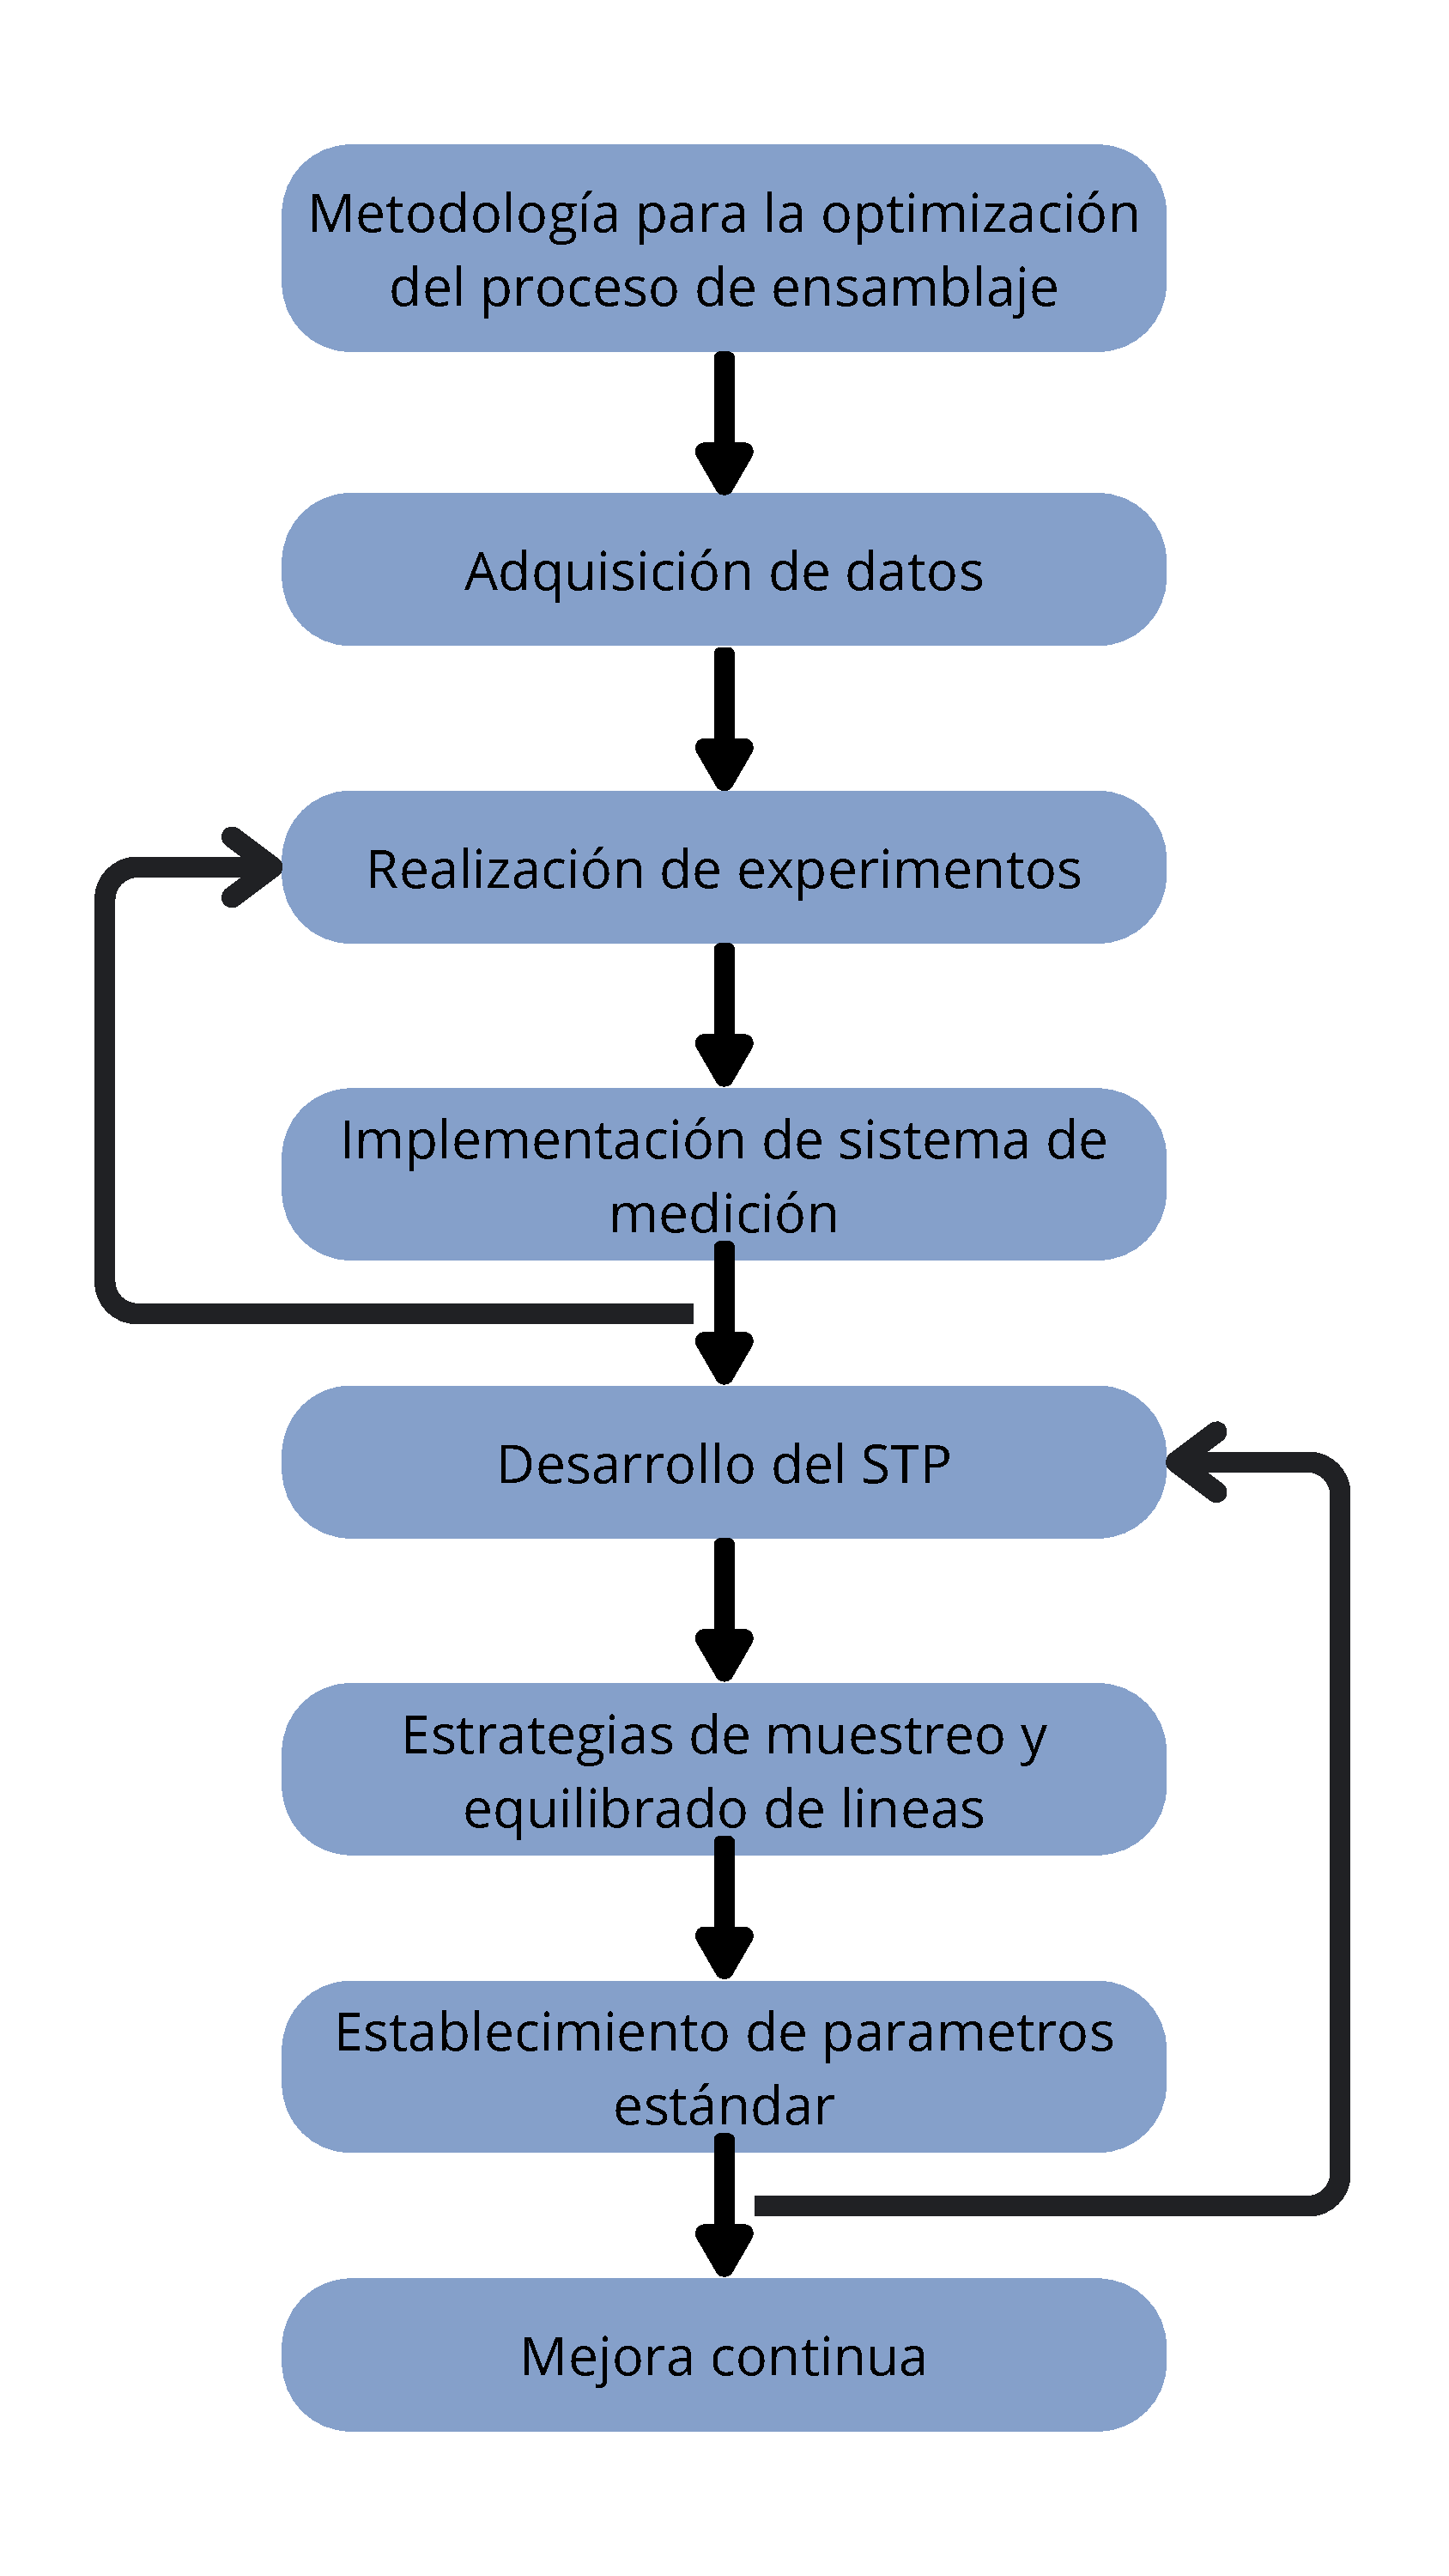
\includegraphics[scale=0.181]{15/img/diagramaMetodologia.pdf}
        \caption{Diagrama de la metodología el desarrollo del sistema.}
        \label{fig:diagramaMetodologia}
    \end{figure}
    
    \subsection{Desarrollo de la guía de plan de Emergencia}
    
    Plan de Respuesta a Emergencia: Documento el cual abordar de manera exhaustiva todas las amenazas, condiciones de vulnerabilidad y riesgos a los que está expuesto el personal en su lugar de trabajo. Asimismo, detalla los recursos disponibles y la formación necesaria para implementar medidas de preparación y respuesta que aseguren la integridad de las personas y minimicen las pérdidas materiales dentro de la Institución, así como estrategias preventivas y correctivas a seguir para garantizar la continuidad operativa del servicio \cite{vra_ucr_emergencias}.
    
    \subsection{Análisis de los métodos, materiales, herramientas e instalación utilizada en la ejecución del ensamble de un circuito electrónico}
    % 
    \subsubsection{Planeación}
    
    Asegúrate de conocer siempre tu objetivo.
    Asegúrate de contar con los documentos (formatos, procedimientos, etc).
    % 
    % 
    \subsubsection{5's}
    % 
    Consiste en tener un lugar de trabajo
    más ordenado, limpio y organizado que
    permite elevar la productividad y
    eficiencia en una empresa, haciéndolo de manera permanente.
    Las etapas son las siguientes: Seleccionar, Ordenar, Limpiar, Estandarizar, y Sostener.
    % 
    \subsubsection{Desarrollo del sistema de tiempos predeterminado}
    %
    
    \begin{figure}[H]
        \centering
        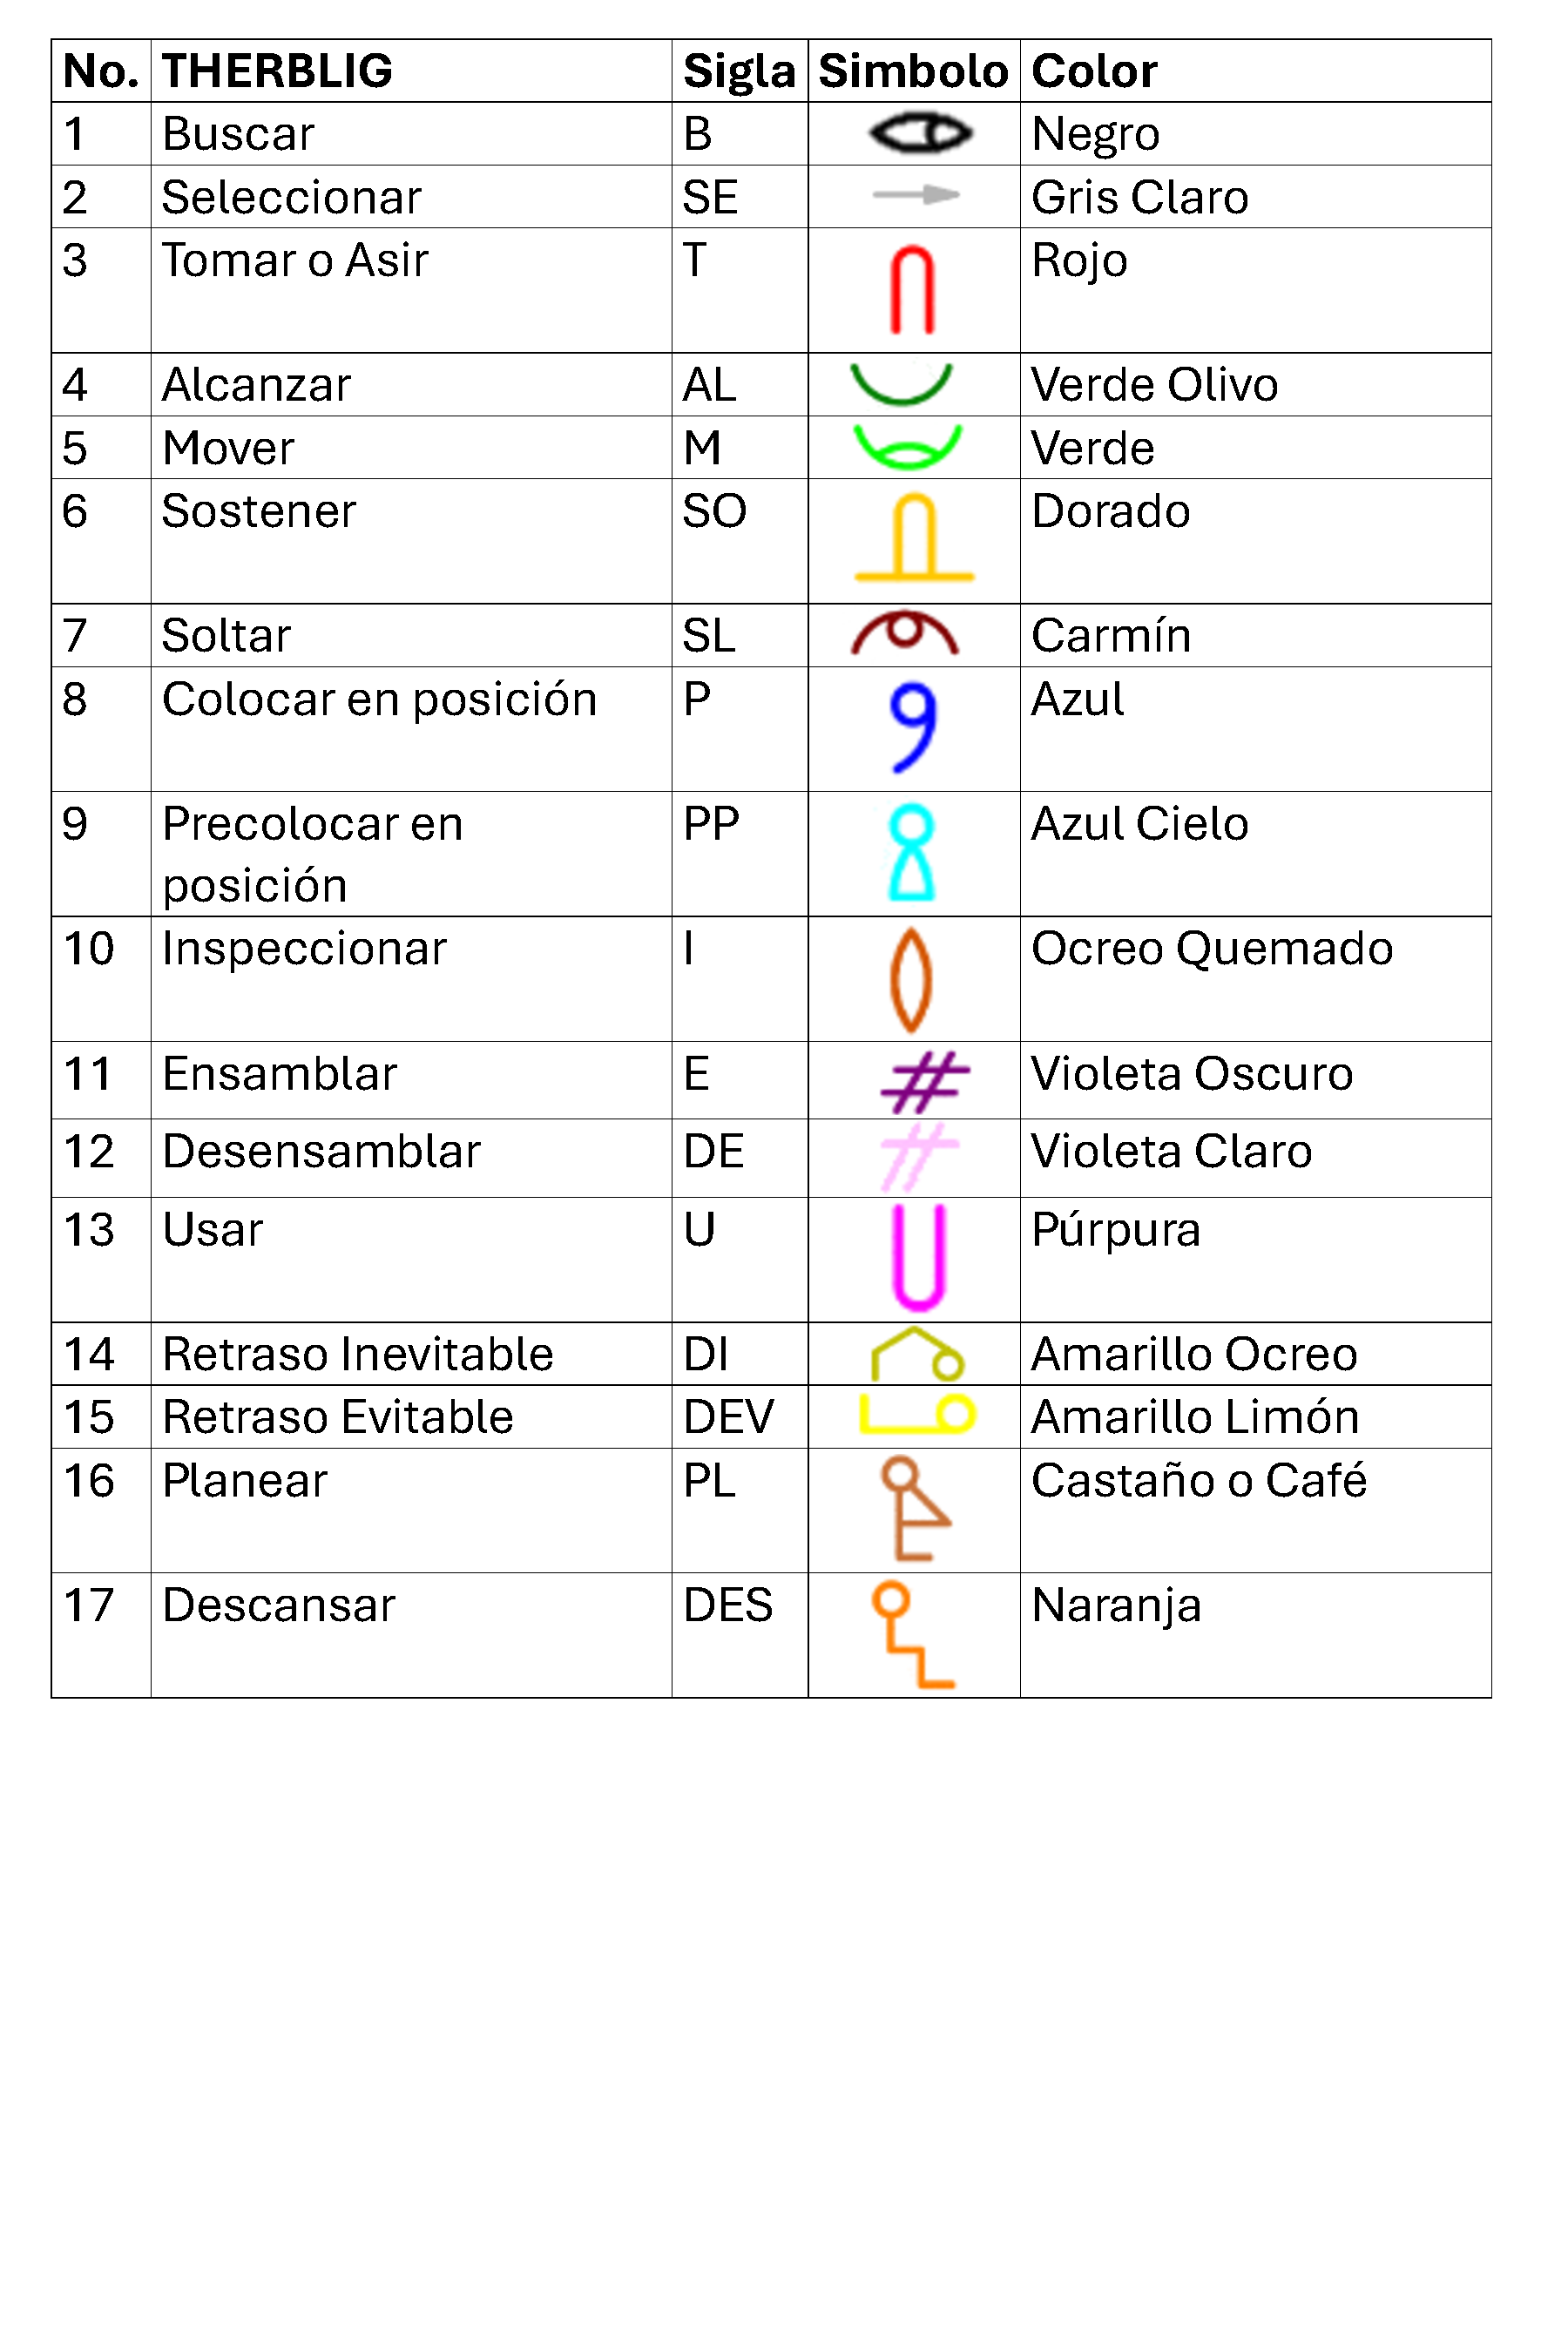
\includegraphics[scale=0.25]{15/img/tablaTherblig.pdf}
        \caption{17 Therbligs.}
        \label{fig:tablaTherbligs}
    \end{figure}
    
    En este sistema el tiempo predeterminado tiene la siguiente descripción y valores equivalentes. Los cuales son utilizados al momento de hacer la toma de tiempos \ref{fig:tablaTMU}.
    
    \begin{figure}[H]
        \centering
        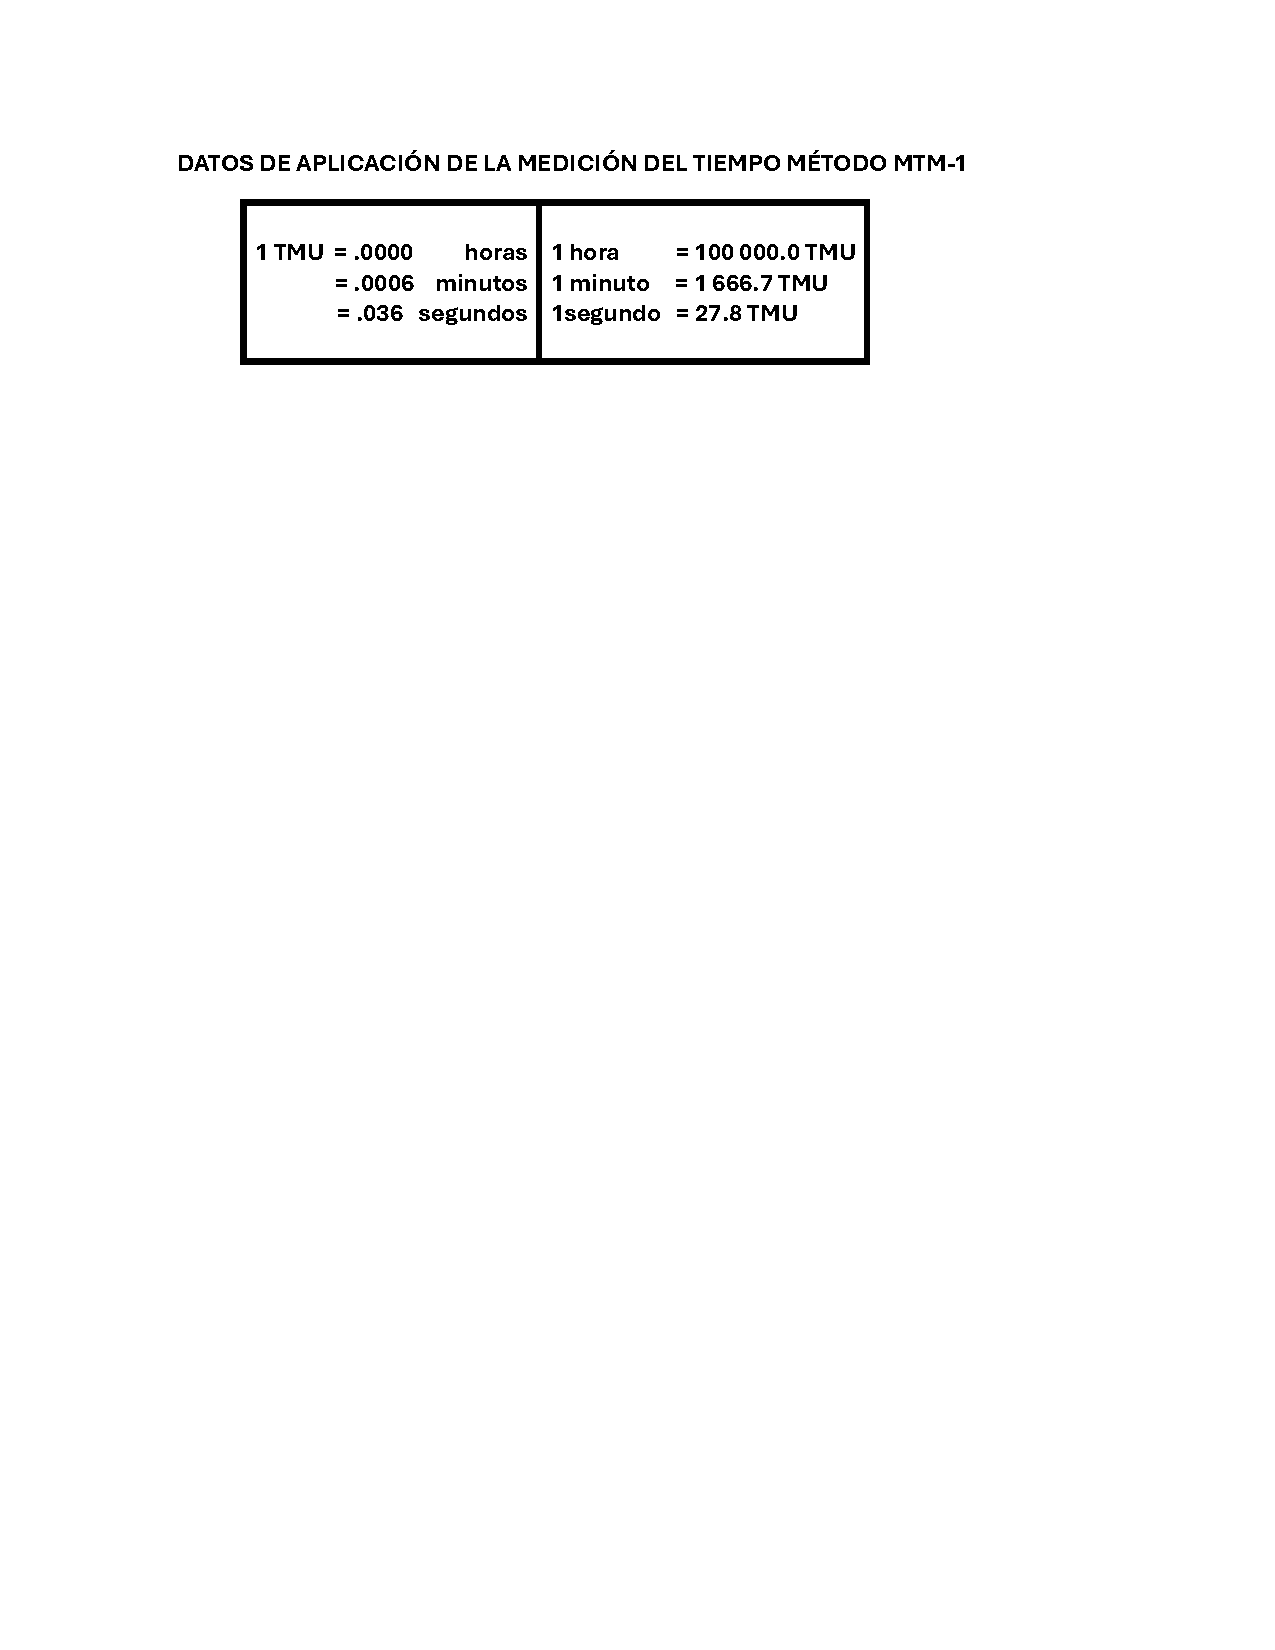
\includegraphics[scale=0.6]{15/img/tablaTMU.pdf}
        \caption{Unidades de Medida De Tiempo (TMU).}
        \label{fig:tablaTMU}
    \end{figure}
    
    Los datos MTM-1 estándar que empleamos para nuestra toma de tiempos, así como el formato para determinar su símbolo con este tipo de sistema en base a cada tipo de movimiento empleado se muestran en las siguientes tablas:
    
    
    \begin{figure}[H]
        \centering   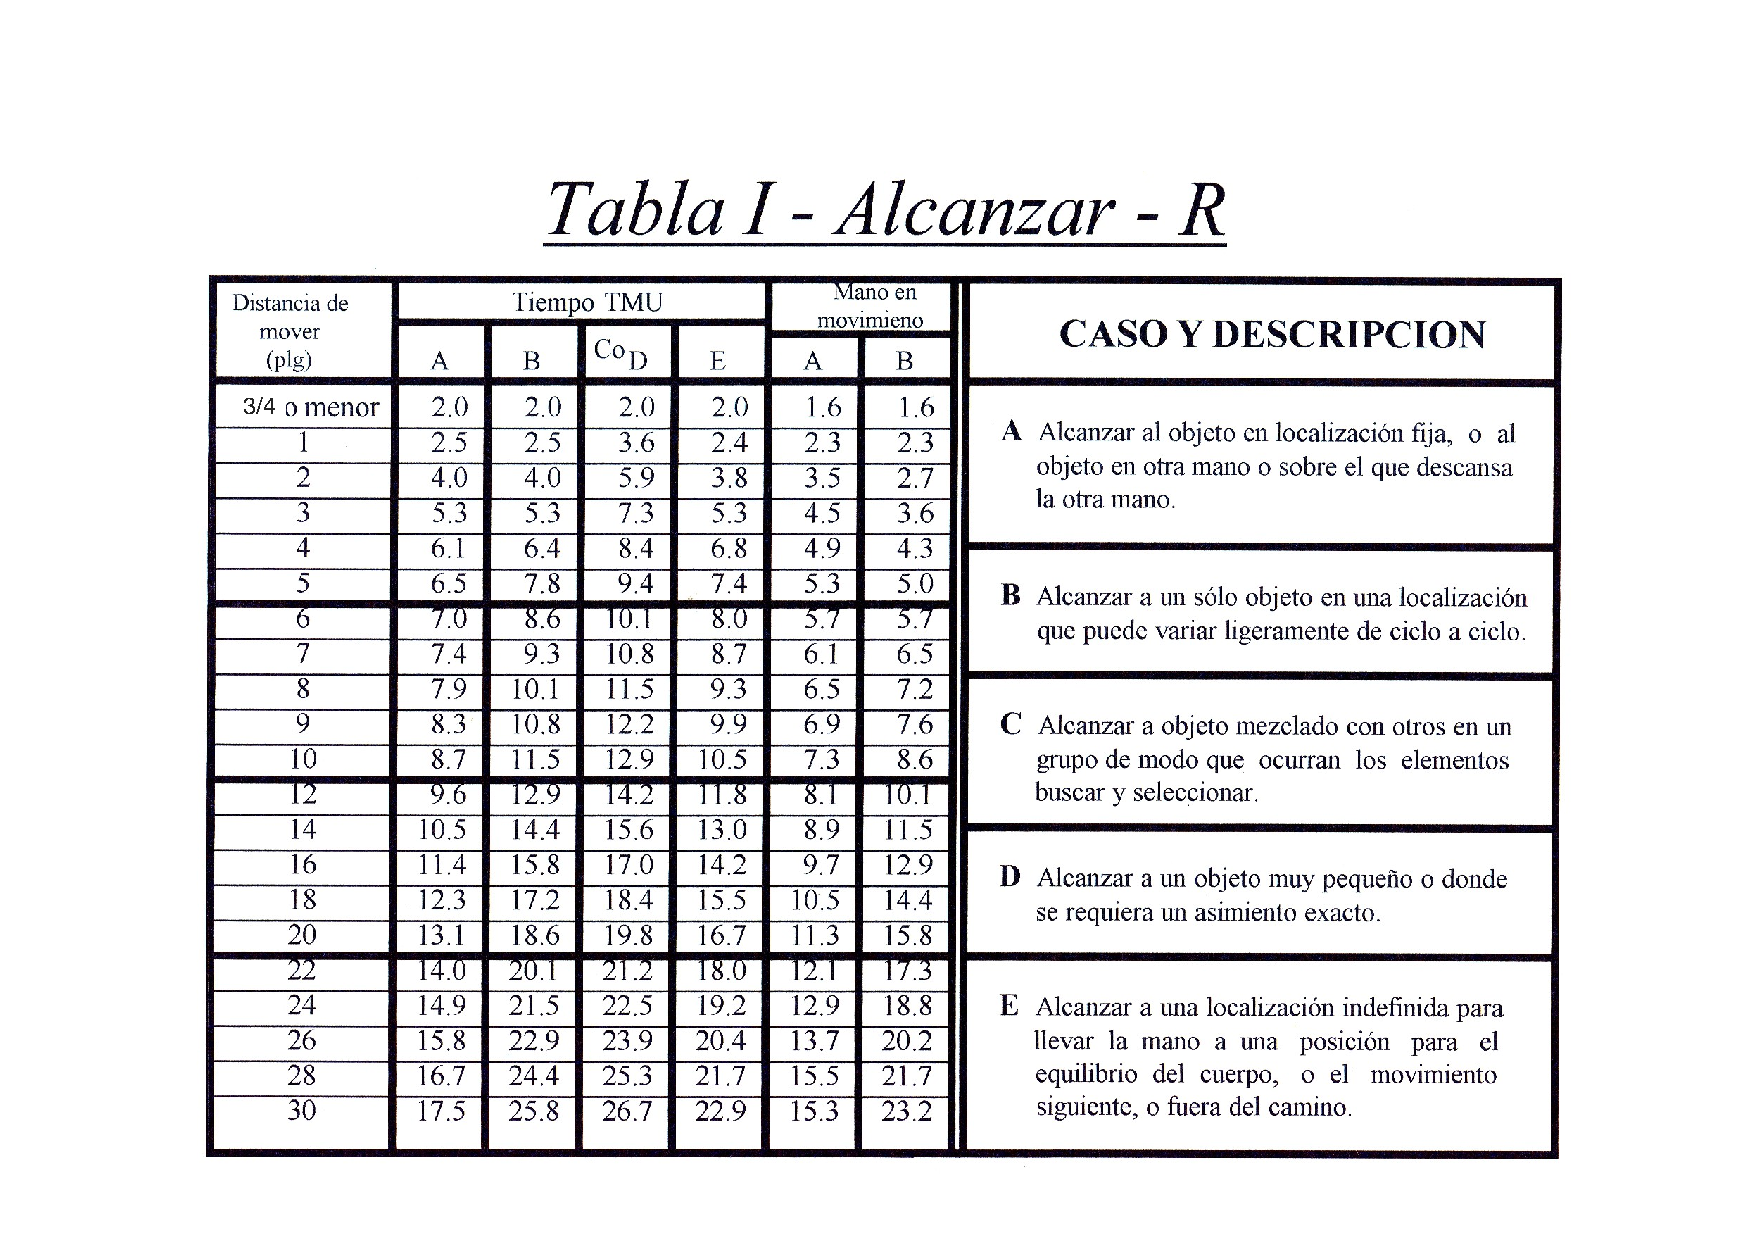
\includegraphics[scale=0.19]{15/img/tabla1Alcanzar.pdf}
        \caption{Alcanzar: Movimiento con la mano vacía desde y hacia el objeto.
        Formato: ALCANZAR/REACH (R): LITERAL/DISTANCIA/CASO}
        \label{fig:tabla1Alcanzar}
    \end{figure}
    
    
    \begin{figure}[H]
        \centering
        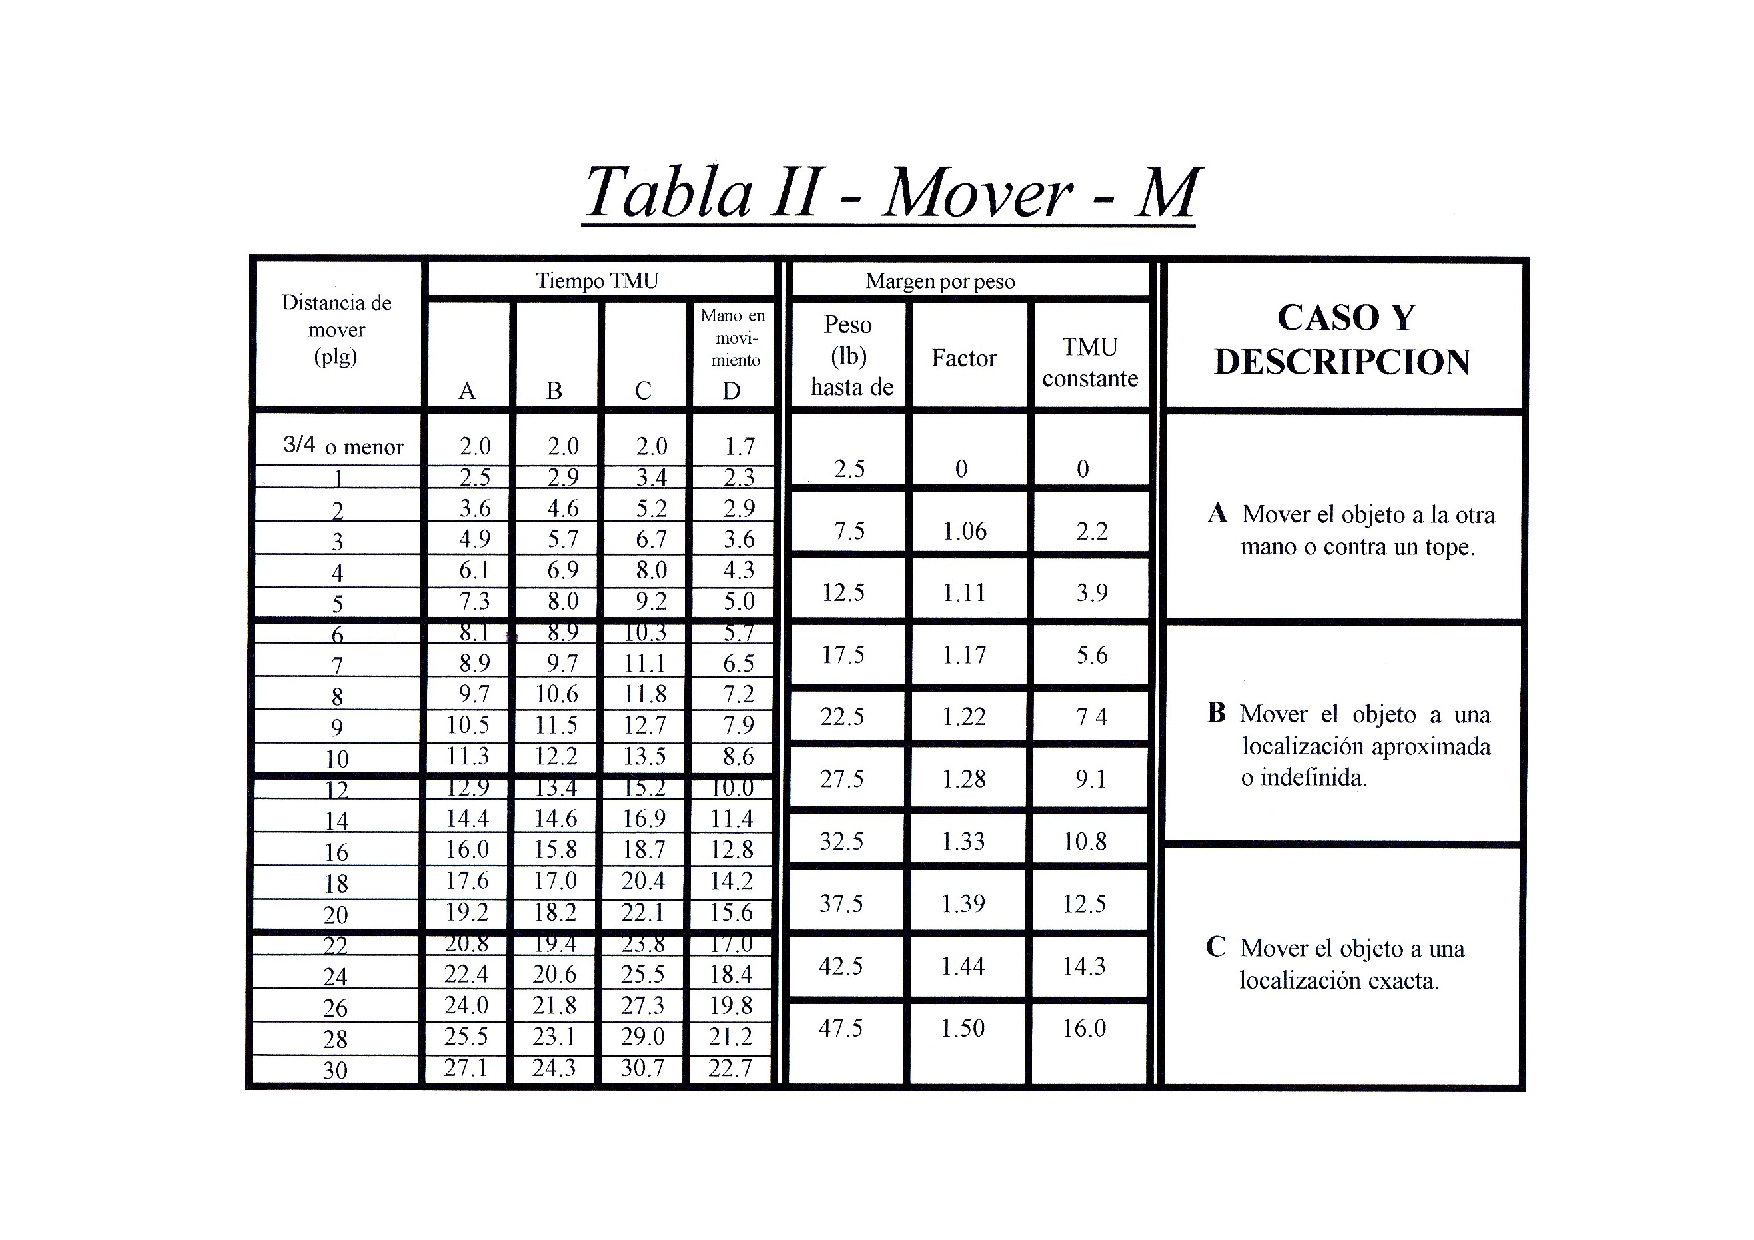
\includegraphics[scale=0.19]{15/img/tabla2Mover.pdf}
        \caption{Mover: Movimiento con mano llena. Formato: MOVER/MOVE (M): LITERAL/DISTANCIA/CASO}
        \label{fig:tabla2Mover}
    \end{figure}
    
    
    \begin{figure}[H]
        \centering
        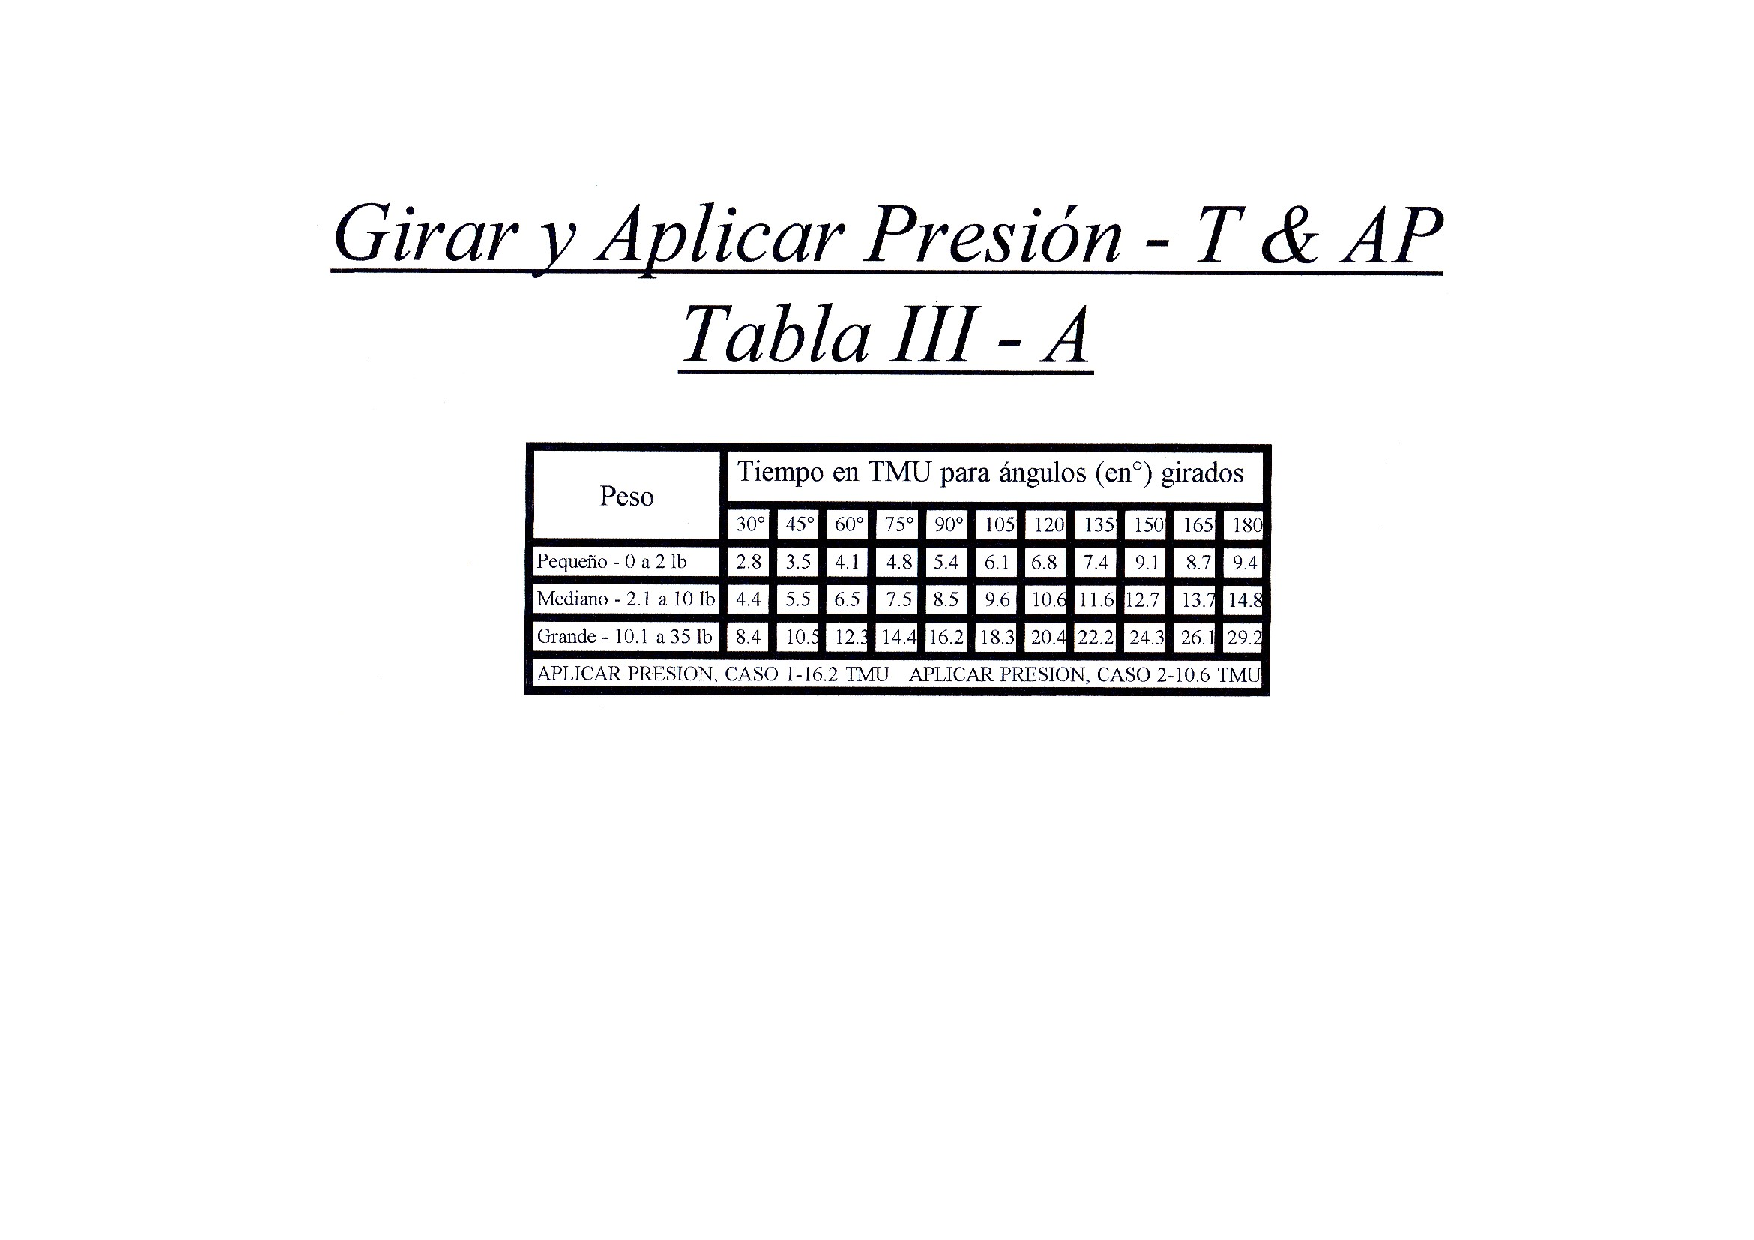
\includegraphics[scale=0.38]{15/img/tabla3GirarAplicarPresion-A.pdf}
        \caption{Girar: Girar la mano respecto al eje largo del antebrazo. Formato: GIRAR/TWIST (T): LITERAL / PESO / ° GIRADOS}
        \label{fig:tabla3GirarAplicarPresion-A}
    \end{figure}
    
    
    \begin{figure}[H]
        \centering
        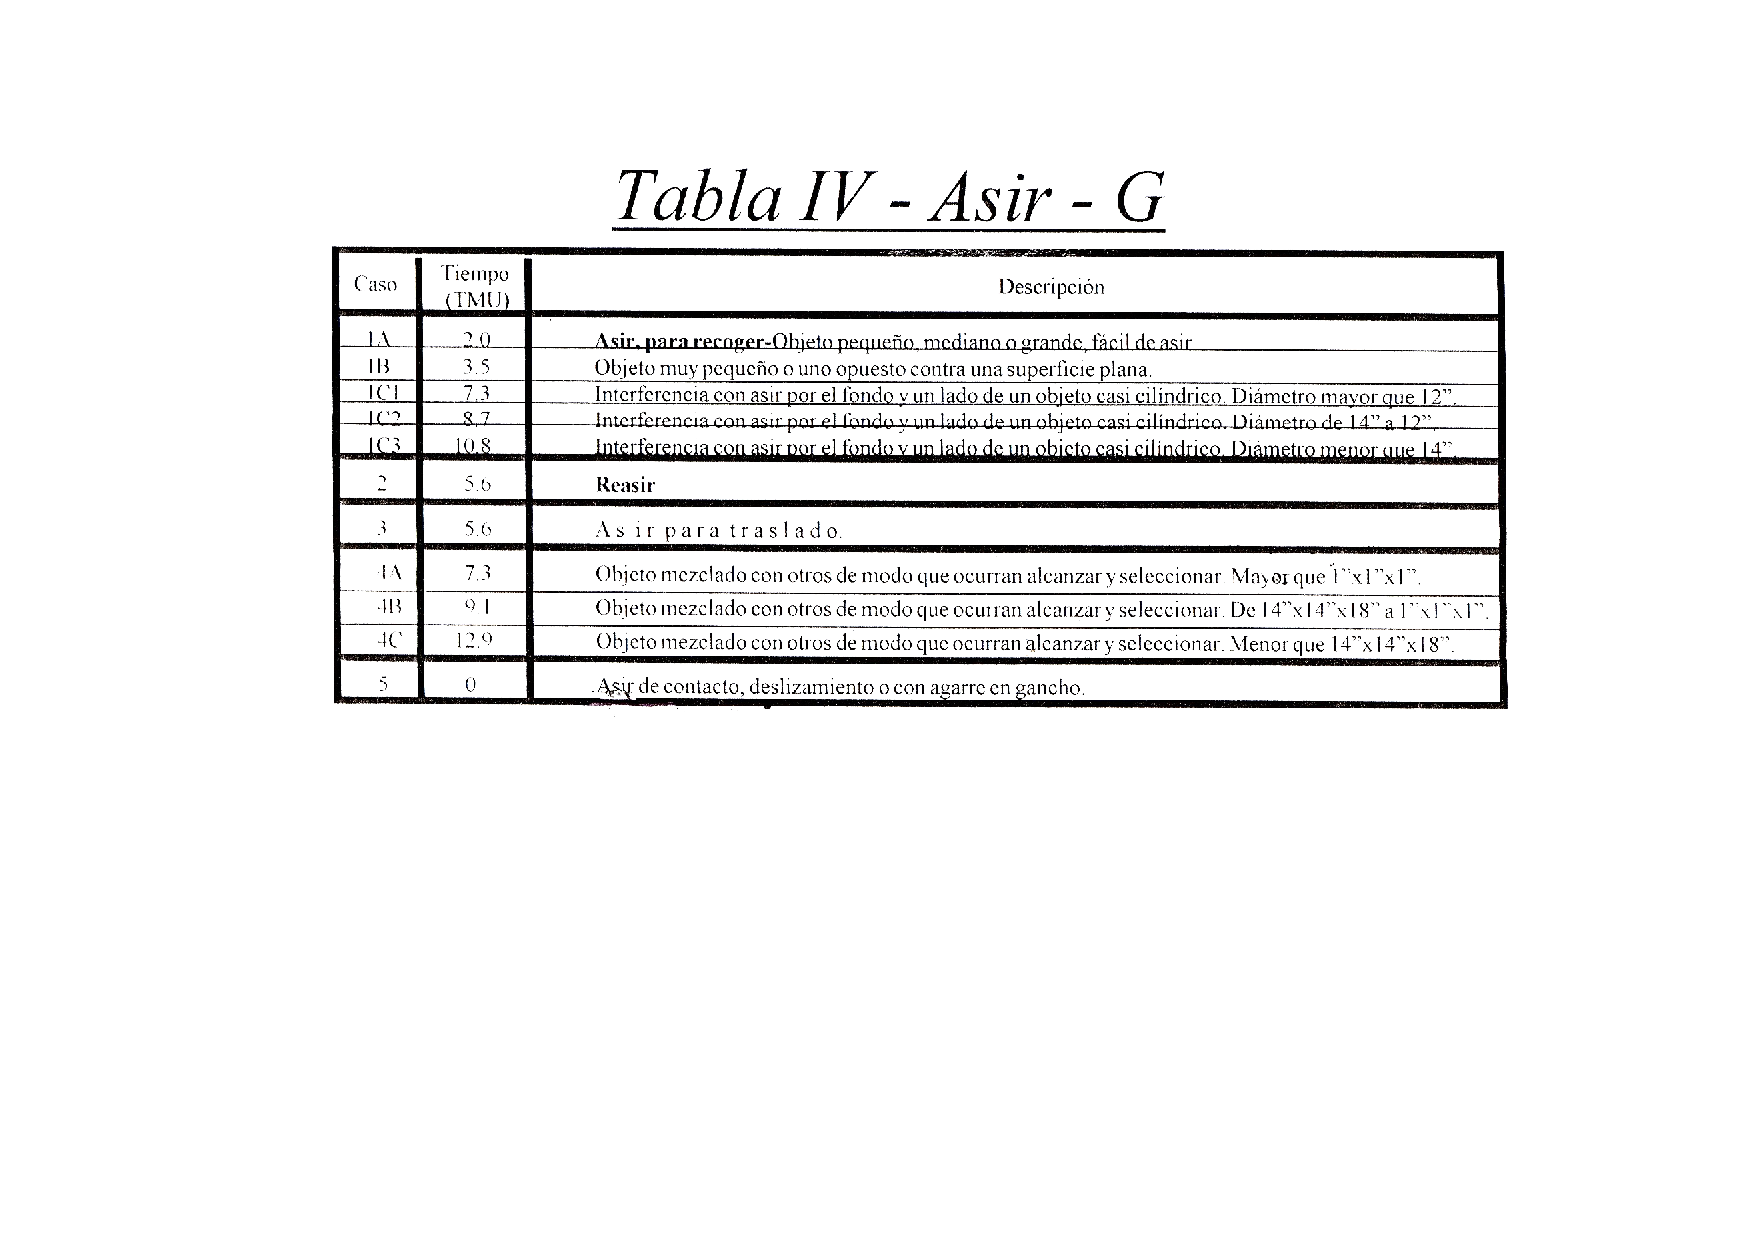
\includegraphics[scale=0.35]{15/img/tabla4Asir.pdf}
        \caption{Asir: Control de uno o más objetos con los dedos o mano, prender. Formato: ASIR/GRIP (G): LITERAL/CASO}
        \label{fig:tabla4Asir}
    \end{figure}
    
    
    \begin{figure}[H]
        \centering
        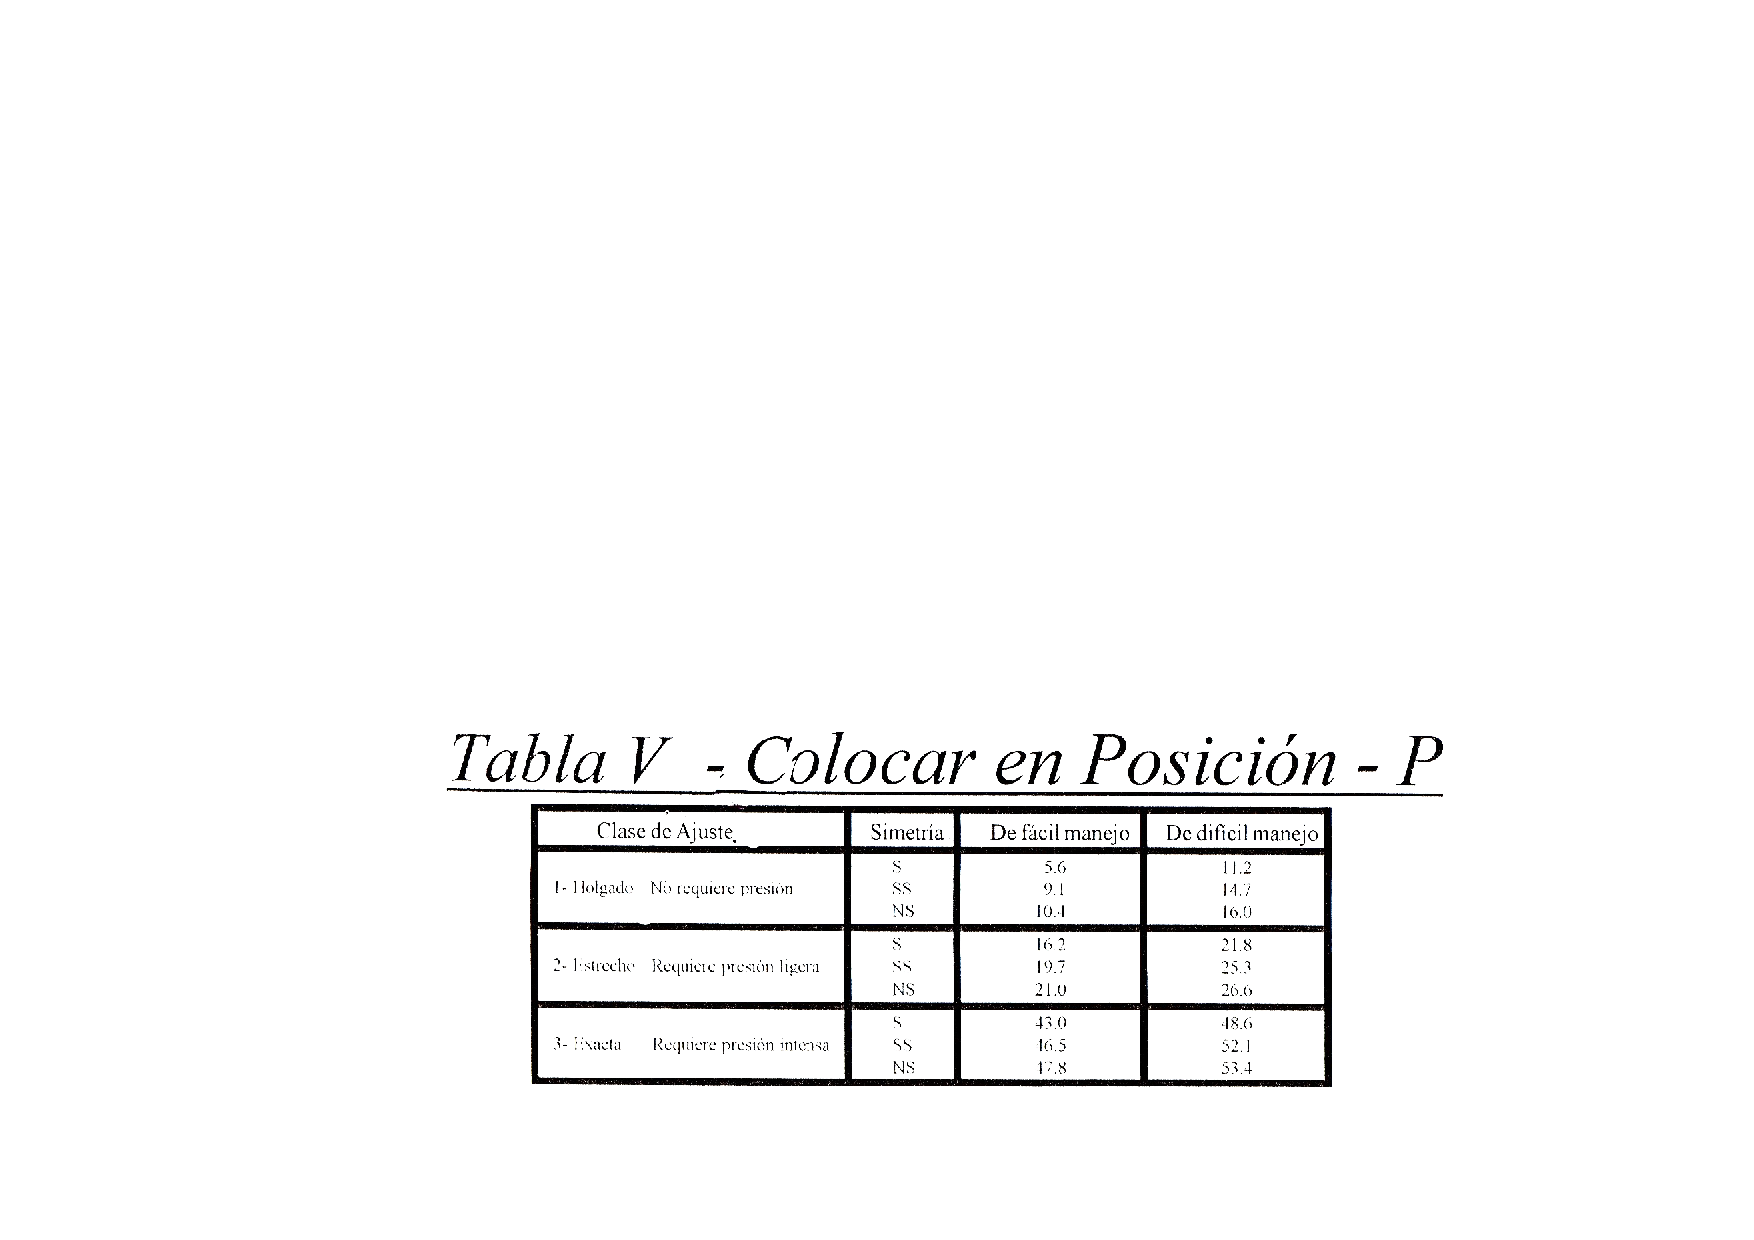
\includegraphics[scale=0.4]{15/img/tabla5ColocarPosicion.pdf}
        \caption{Colocar en posición: Alinear, orientar o engranar un objeto con otro: COLOCAR EN POSICIÓN/PUT (P): LITERAL/CLASE DE AJUSTE/SIMETRÍA/MANEJO}
        \label{fig:tabla5ColocarPosicion}
    \end{figure}
    
    \begin{figure}[H]
       \centering
        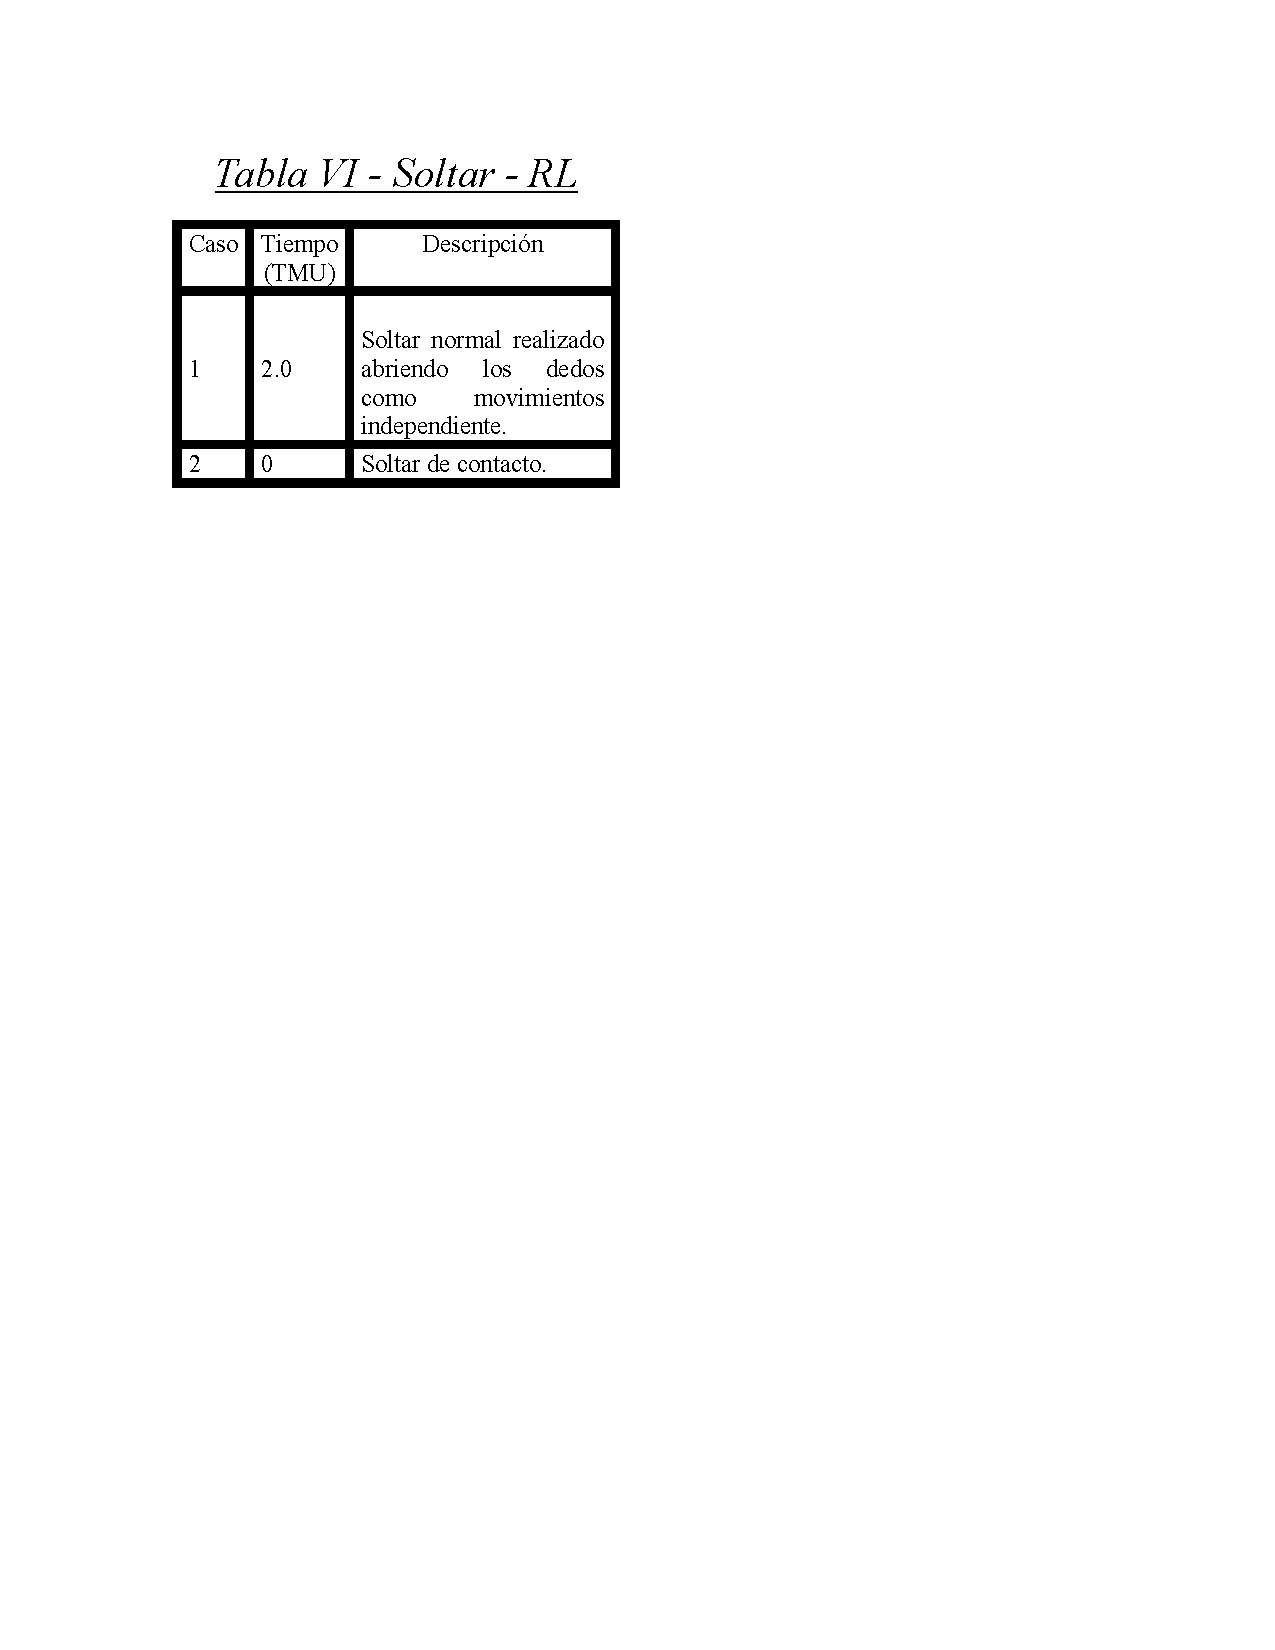
\includegraphics[scale=0.65]{15/img/tabla6Soltar.pdf}
        \caption{Soltar: Entregar el control de un objeto. Formato: SOLTAR/RELEASE (RL): LITERAL/CASO}
        \label{fig:tabla6Soltar}
    \end{figure}
    
    \begin{figure}[H]
       \centering
        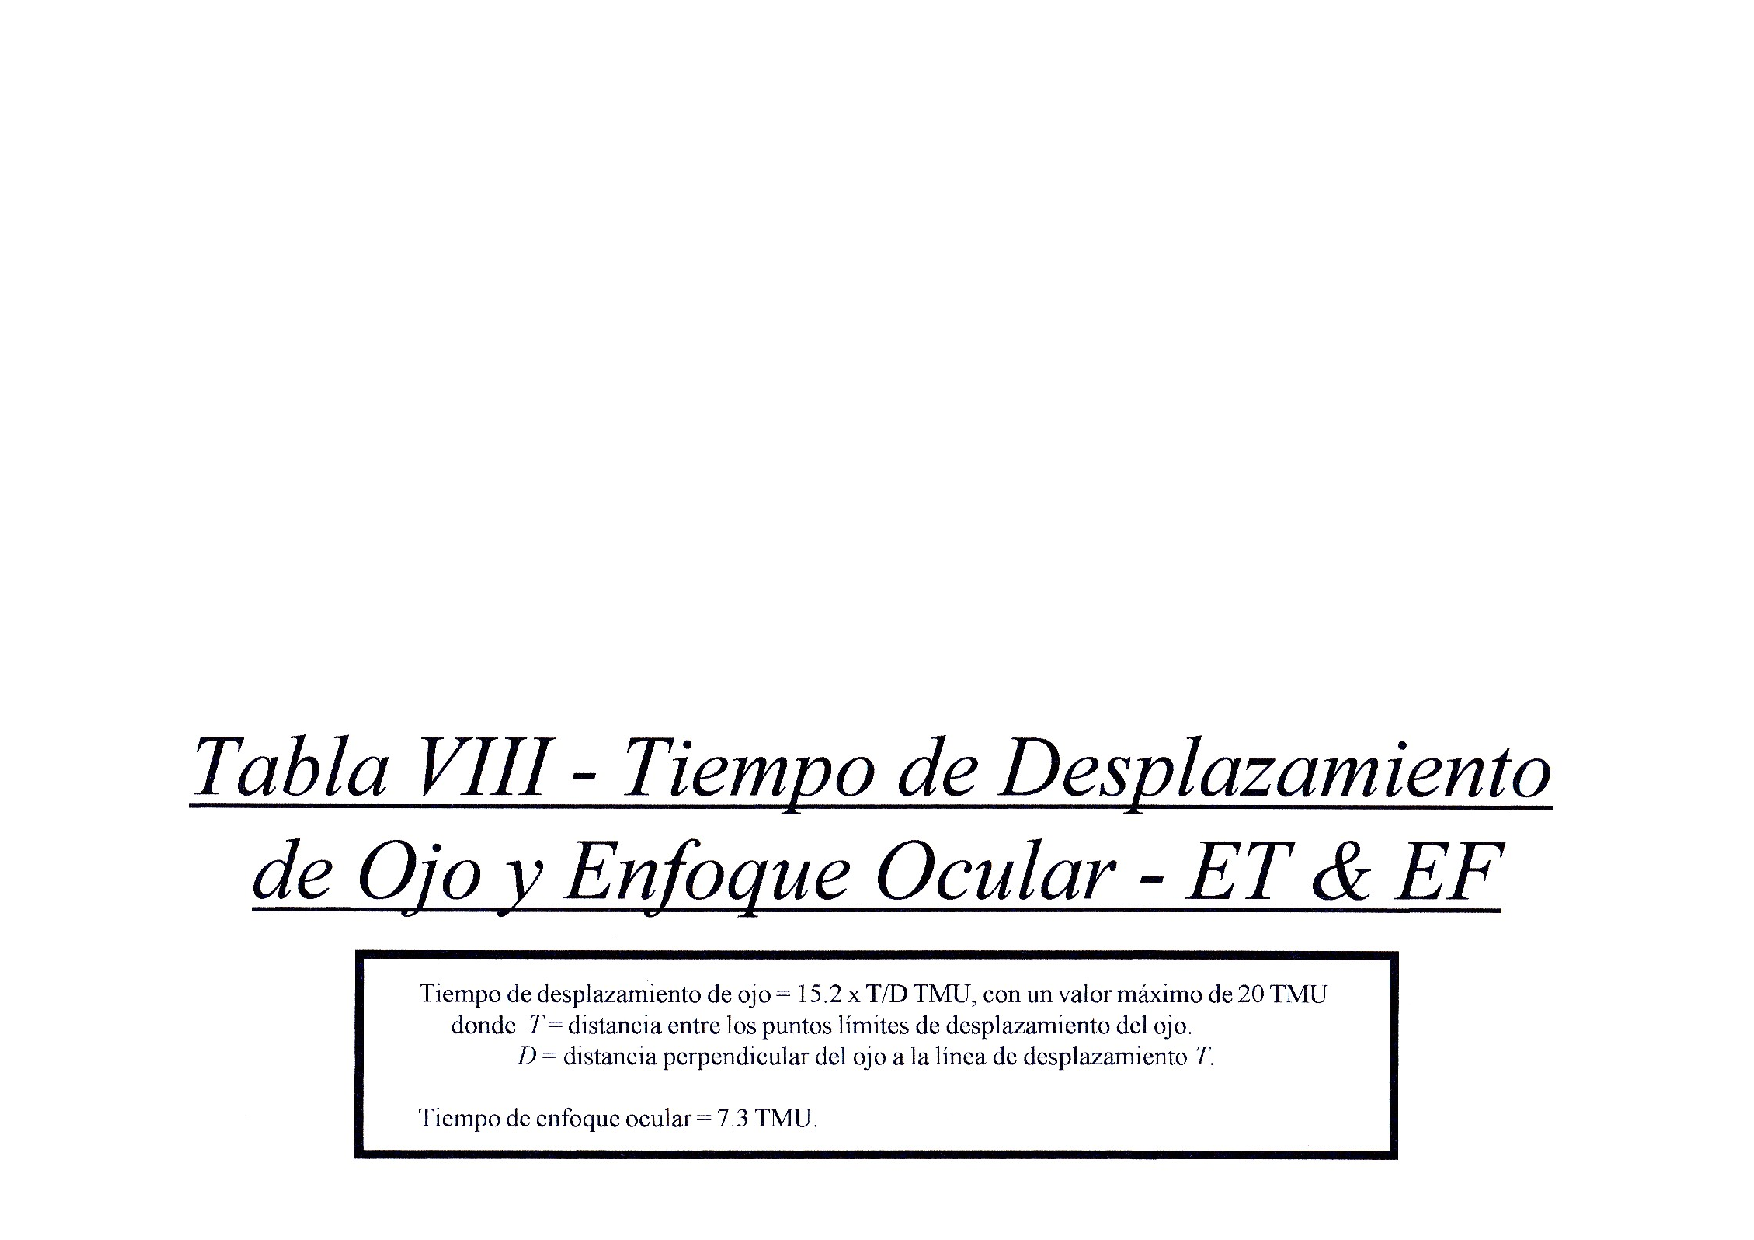
\includegraphics[scale=0.3]{15/img/tabla8TiempoDesplazamientoOjo.pdf}
        \caption{Enfoque Ocular: Elemento visual y mental, de mirar hacia un objeto el tiempo suficiente para determinar una característica fácilmente visible.}
        \label{fig:tabla8TiepoDesplazamientoOjo}
    \end{figure}
    
    Se coloca la sigla o inicial de la palabra del idioma ingles que significa el movimiento fundamental véase el siguiente ejemplo \ref{fig:tabla1AlcanzarEjemplo}.
    
    \begin{figure}[H]
       \centering
        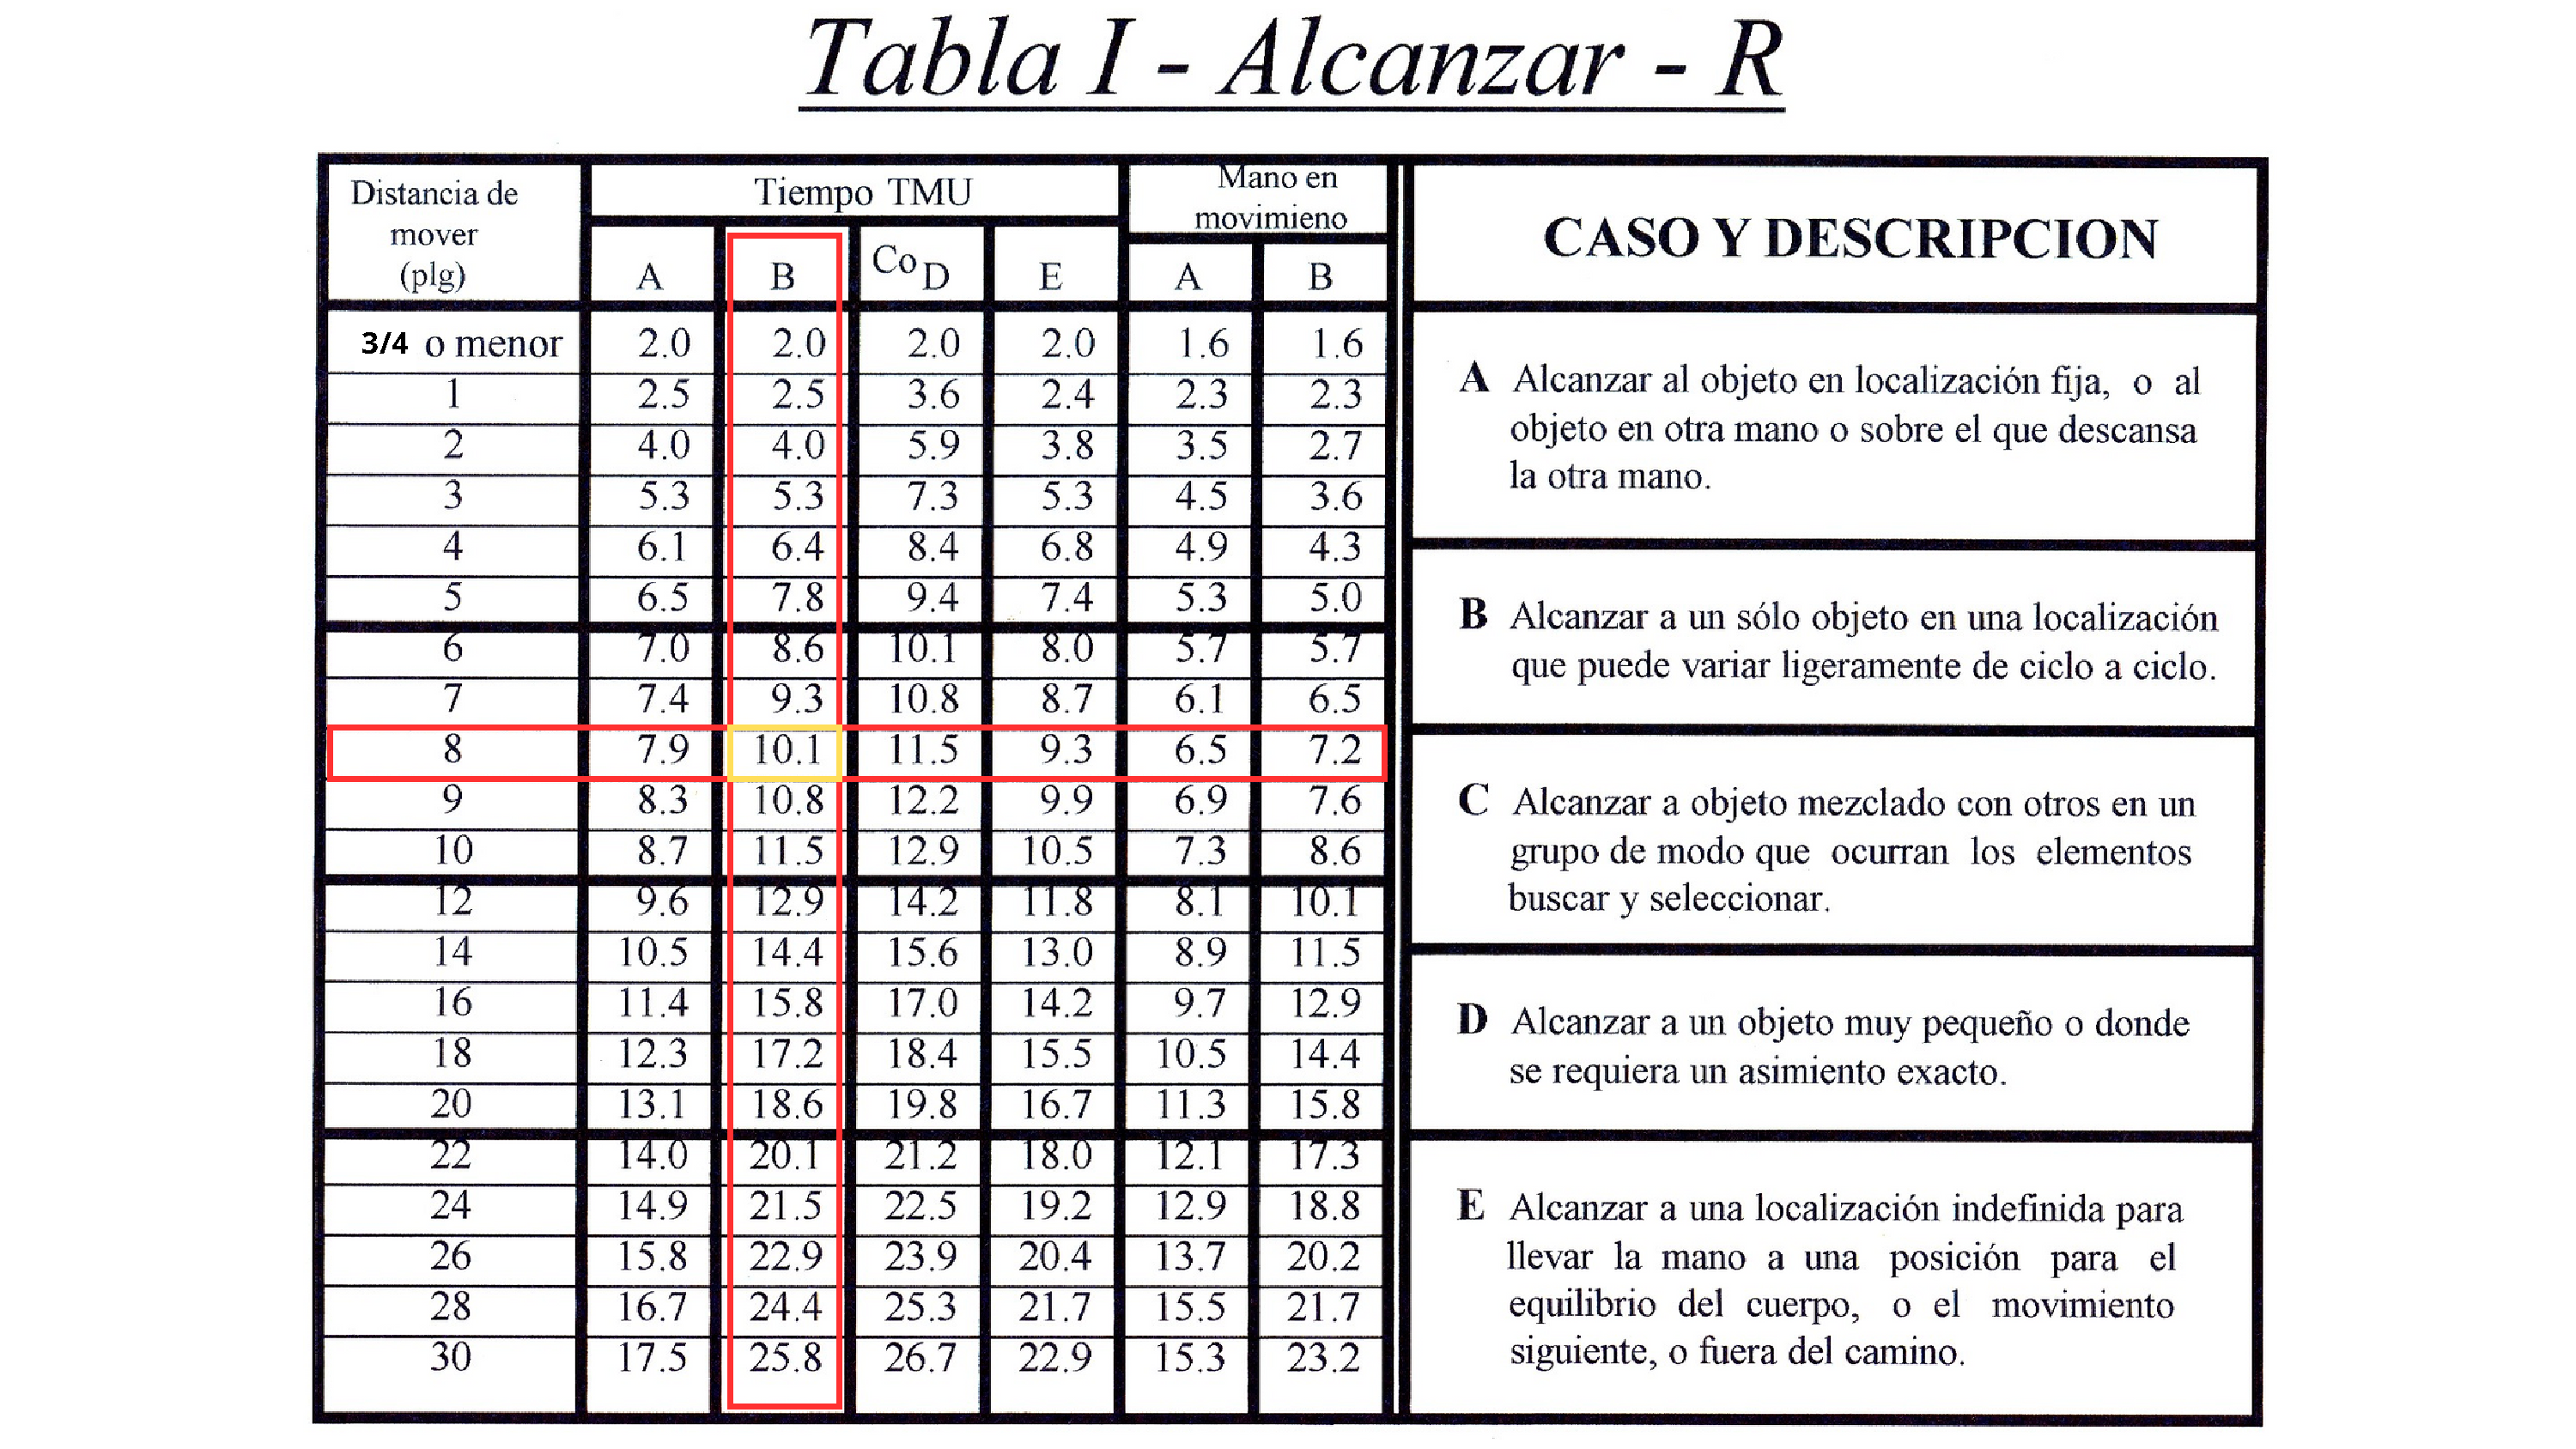
\includegraphics[scale=0.19]{15/img/tabla1AlcanzarEjemplo.pdf}
        \caption{Alcanzar un objeto en localización fija a una distancia de 8 pulgadas, se codifica como: R8A = 10.1 TMU}
        \label{fig:tabla1AlcanzarEjemplo}
    \end{figure}
    
    
    El formato para el registro de tiempos en MTM se conoce como Hoja de análisis de métodos, debe contener: descripción de la operación, símbolo (utilizando el formato correspondientes) y tiempo (TMU) véase en la Figura \ref{fig:formatoRegistroMTM}. 
    
    \begin{figure}[H]
       \centering
        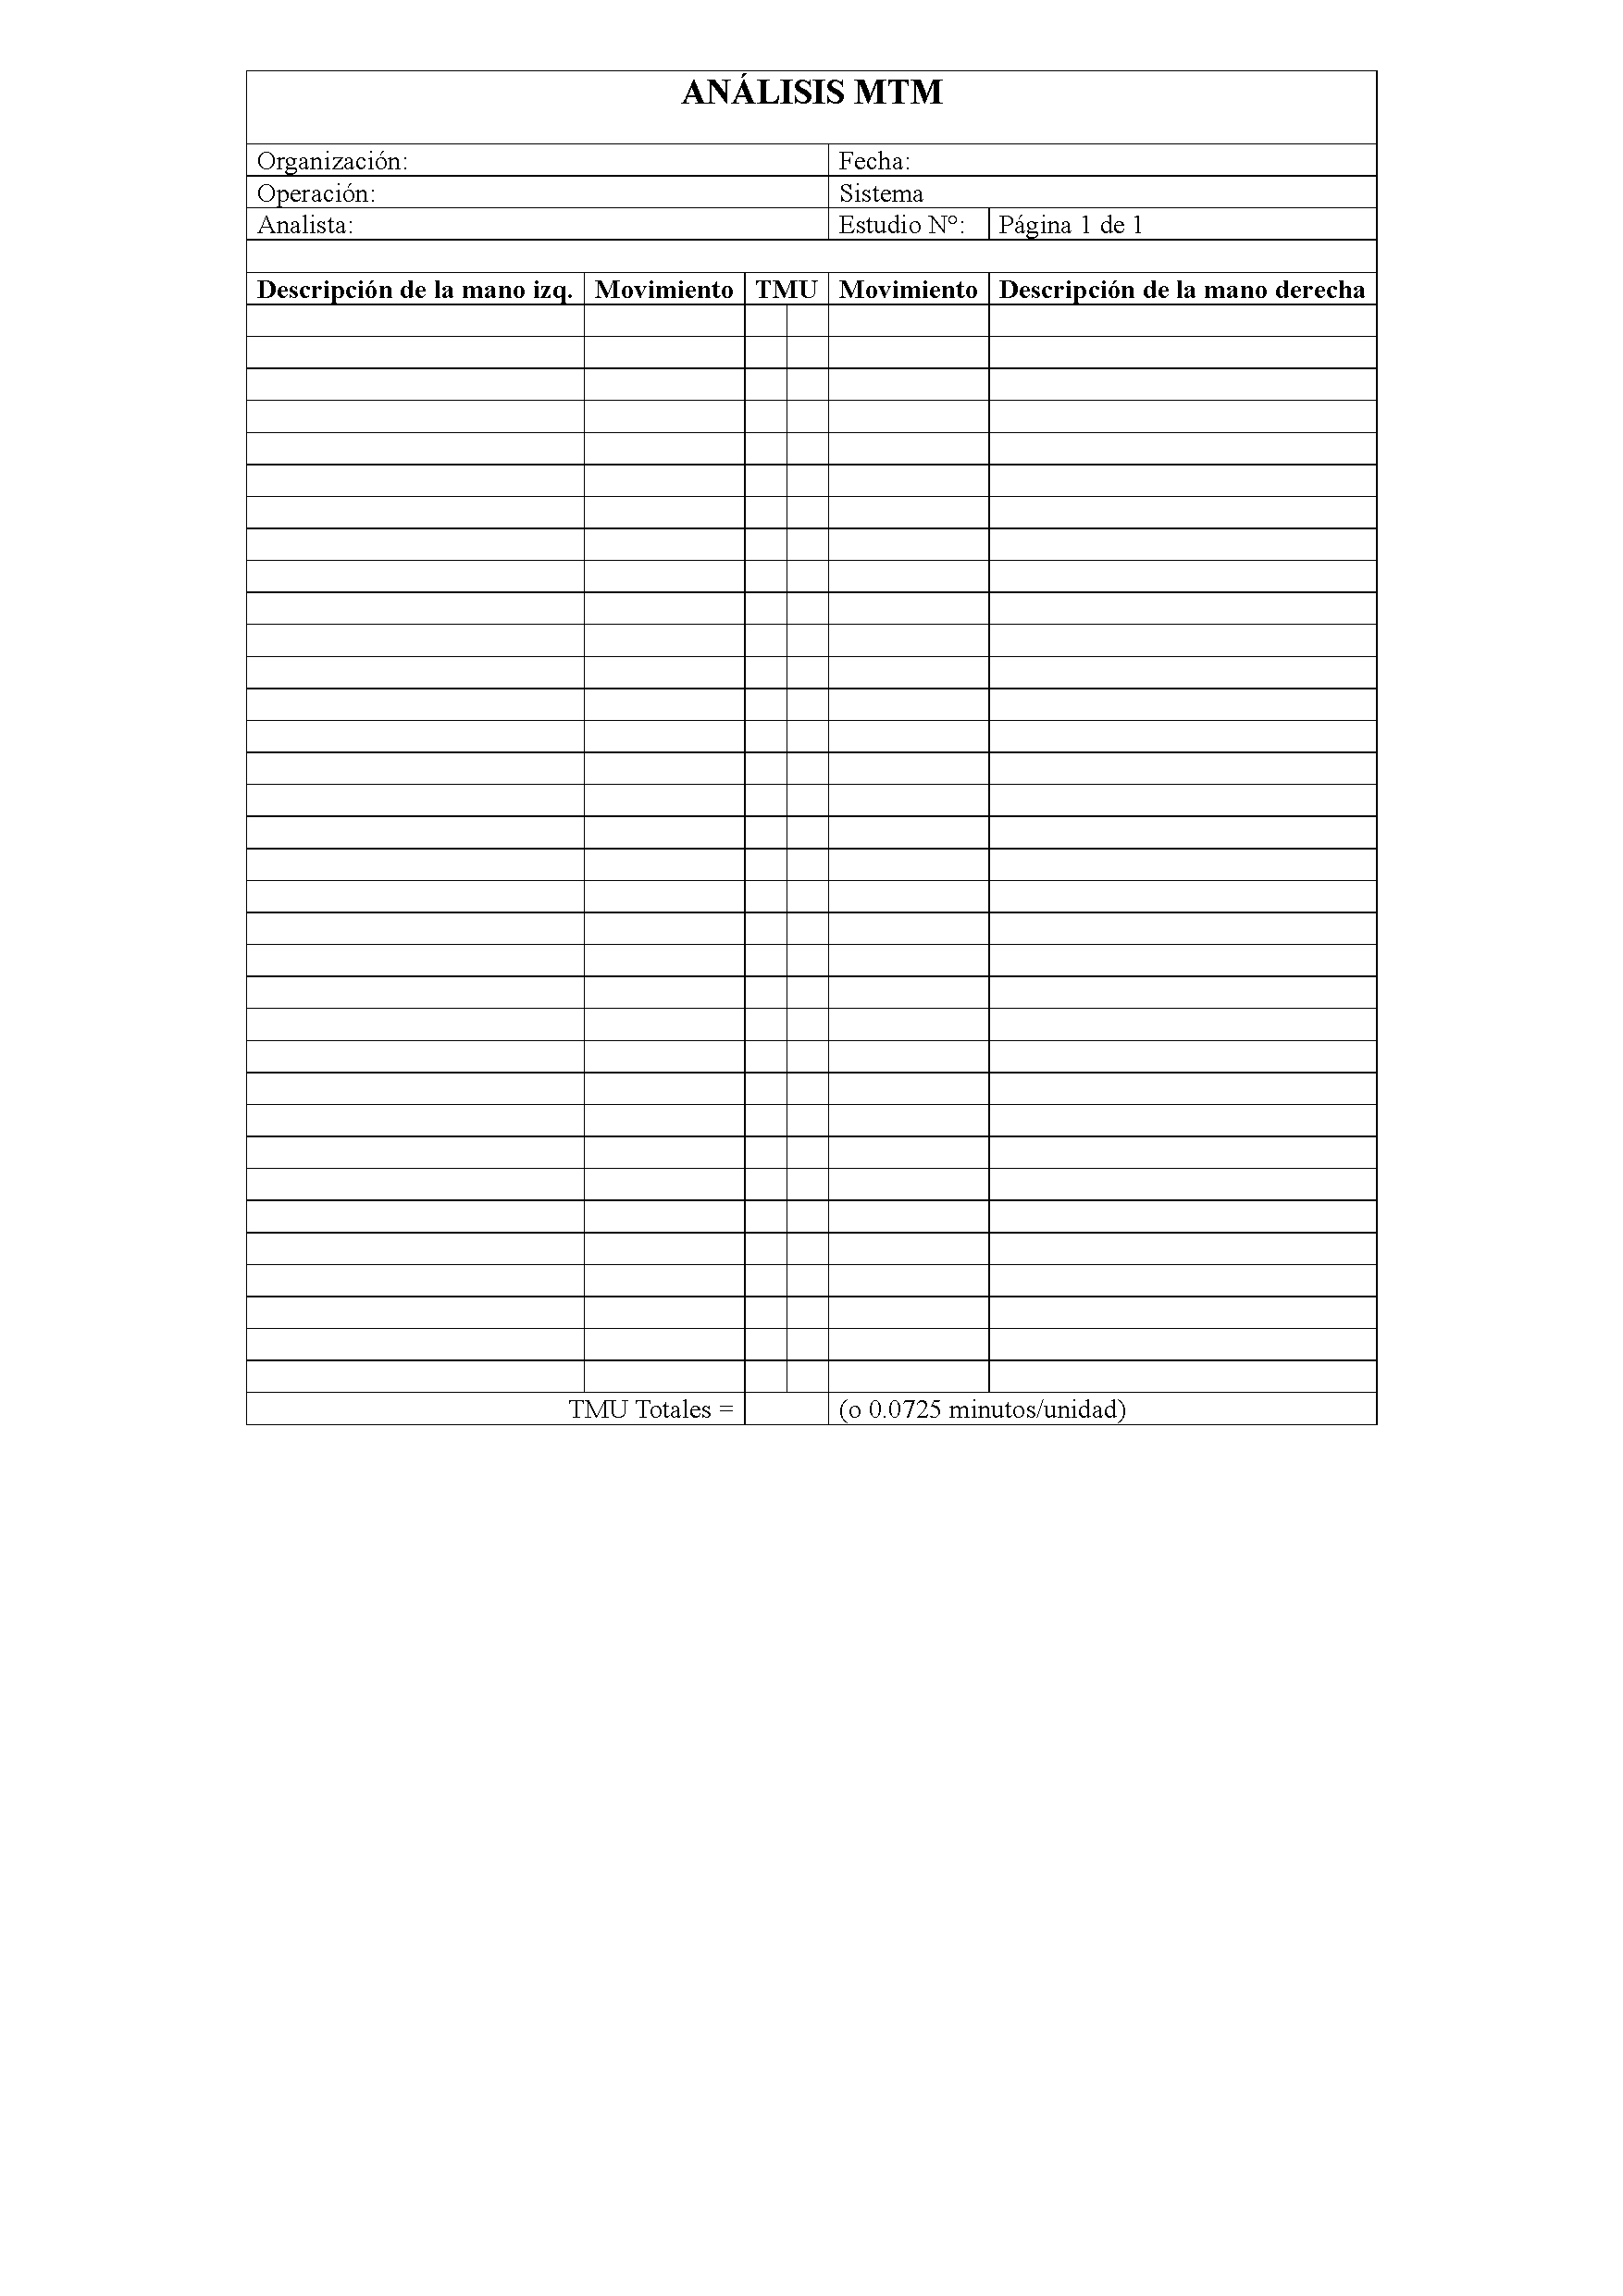
\includegraphics[scale=0.3]{15/img/formatoRegistroMTM.pdf}
        \caption{Hoja de análisis de métodos.}
        \label{fig:formatoRegistroMTM}
    \end{figure}
    
    
    La ley por la que se rige el uso de los movimientos en el MTM es: ¨Principio de la reducción de movimientos¨ \cite{estudio_del_trabajo_ii}.
    % 
    \subsubsection{Desarrollo del muestreo del trabajo}
    % 
    El muestreo del trabajo es una técnica utilizada en la ingeniería industrial y en la gestión de operaciones para analizar la utilización del tiempo de trabajo y determinar la eficiencia de los procesos. Esta técnica implica observar y registrar, en momentos aleatorios, lo que están haciendo los trabajadores o cómo se están utilizando las máquinas y otros recursos. A partir de estas observaciones, se puede estimar la proporción del tiempo dedicado a diferentes actividades, tanto productivas como no productivas. En el contexto del proyecto integrador, el muestreo del trabajo se convierte en una herramienta esencial para identificar ineficiencias, cuellos de botella y oportunidades de mejora \cite{muestreo-trabajo}.
    % 
    \subsubsection{Corrección por balanceo de procesos}
    %
    La corrección por balanceo de procesos es una técnica utilizada en la gestión de operaciones y la ingeniería industrial para optimizar la distribución de trabajo a lo largo de una línea de producción o ensamble. El objetivo principal del balanceo de procesos es minimizar los tiempos de inactividad y desequilibrios entre estaciones de trabajo, asegurando que cada estación tenga una carga de trabajo equilibrada y que el flujo de producción sea lo más continuo y eficiente posible. En el proyecto integrador, aplicar el balanceo de procesos es crucial para mejorar la eficiencia y la productividad \cite{balanceo-procesos}.
    % 
    \subsubsection{Datos estándar continuos y discretos}
    % 
    Los datos estándar continuos y discretos son dos formas de medir y representar el tiempo utilizado en procesos de producción, como el ensamblaje electrónico. Cada tipo de datos estándar tiene características específicas y se utiliza en diferentes contextos \cite{datos-estandar}.
    
    \begin{enumerate}
        \item Datos Estándar Continuos: Estos datos representan el tiempo en unidades continuas, como minutos o segundos. Se utilizan para medir tareas que fluyen de manera continua y no se pueden dividir fácilmente en partes discretas. Por ejemplo, el tiempo necesario para ensamblar un componente electrónico puede medirse en minutos o segundos.
    
        \item Datos Estándar Discretos: Estos datos representan el tiempo en unidades discretas, como unidades de trabajo o movimientos individuales. Se utilizan para medir tareas que pueden descomponerse en pasos o movimientos separados. Por ejemplo, el tiempo necesario para conectar un cable en un ensamble electrónico puede medirse en unidades discretas.
     
    \end{enumerate}
    % 
    % 
    \subsection{Diseño de la forma más económica de realizar el trabajo}
    % 
    Después de hacer el ensamble y hacer el análisis de los tiempos estándar y tiempos ciclos se hizo un análisis para llevar a cabo una normalización de los materiales con el fin de encontrar la forma mas económica de hacer el trabajo realizando una tabla la cual se encuentra en los resultados de este proyecto y podemos encontrar la comparación de la diferencia de precios, de primera impresión puede parecer que la suma de los materiales para el nuevo ensamble puede ser mayor al viejo ensamble, sin embargo lo que buscamos es anticiparnos a los contratiempos que podemos encontrar los cuales si no tenemos previstos con anticipación pueden resultar mas costosos y generar mas gastos ante la urgencia de querer terminar el ensamble pues compraremos materiales disponibles en vez de comprar los materiales necesarios.
    
    % 
    \subsection{Normalización de los métodos, materiales, herramientas e instalaciones}
    % 
    La normalización de los métodos, materiales, herramientas e instalaciones es crucial para el desarrollo de este proyecto. Este proceso implica la implementación de estándares y procedimientos uniformes que garantizan la calidad, seguridad y eficiencia en cada etapa del ensamblaje. La normalización asegura que los componentes electrónicos sean compatibles y funcionen correctamente, facilita la interoperabilidad entre diferentes partes del circuito y reduce costos al minimizar errores y retrabajos. Además, establece un marco claro para la selección de materiales, el uso de herramientas específicas y la configuración de instalaciones, lo que contribuye a la consistencia y la confiabilidad del proyecto. Al adherirse a normas establecidas, se promueve la innovación y se facilita la integración de nuevas tecnologías en el diseño y fabricación de circuitos electrónicos\cite{normalización}.
    
    
    
    Para este proyecto se utilizaron diversos materiales, los cuales son indespensables para la obtención de un resultado positivo y los objetivos a cumplir, a continuación se muestra una lista de los materiales utilizados en tal proceso vease en la siguiente tabla \ref{fig:listaDeMateriales}.
    
    \begin{figure}[H]
        \centering
        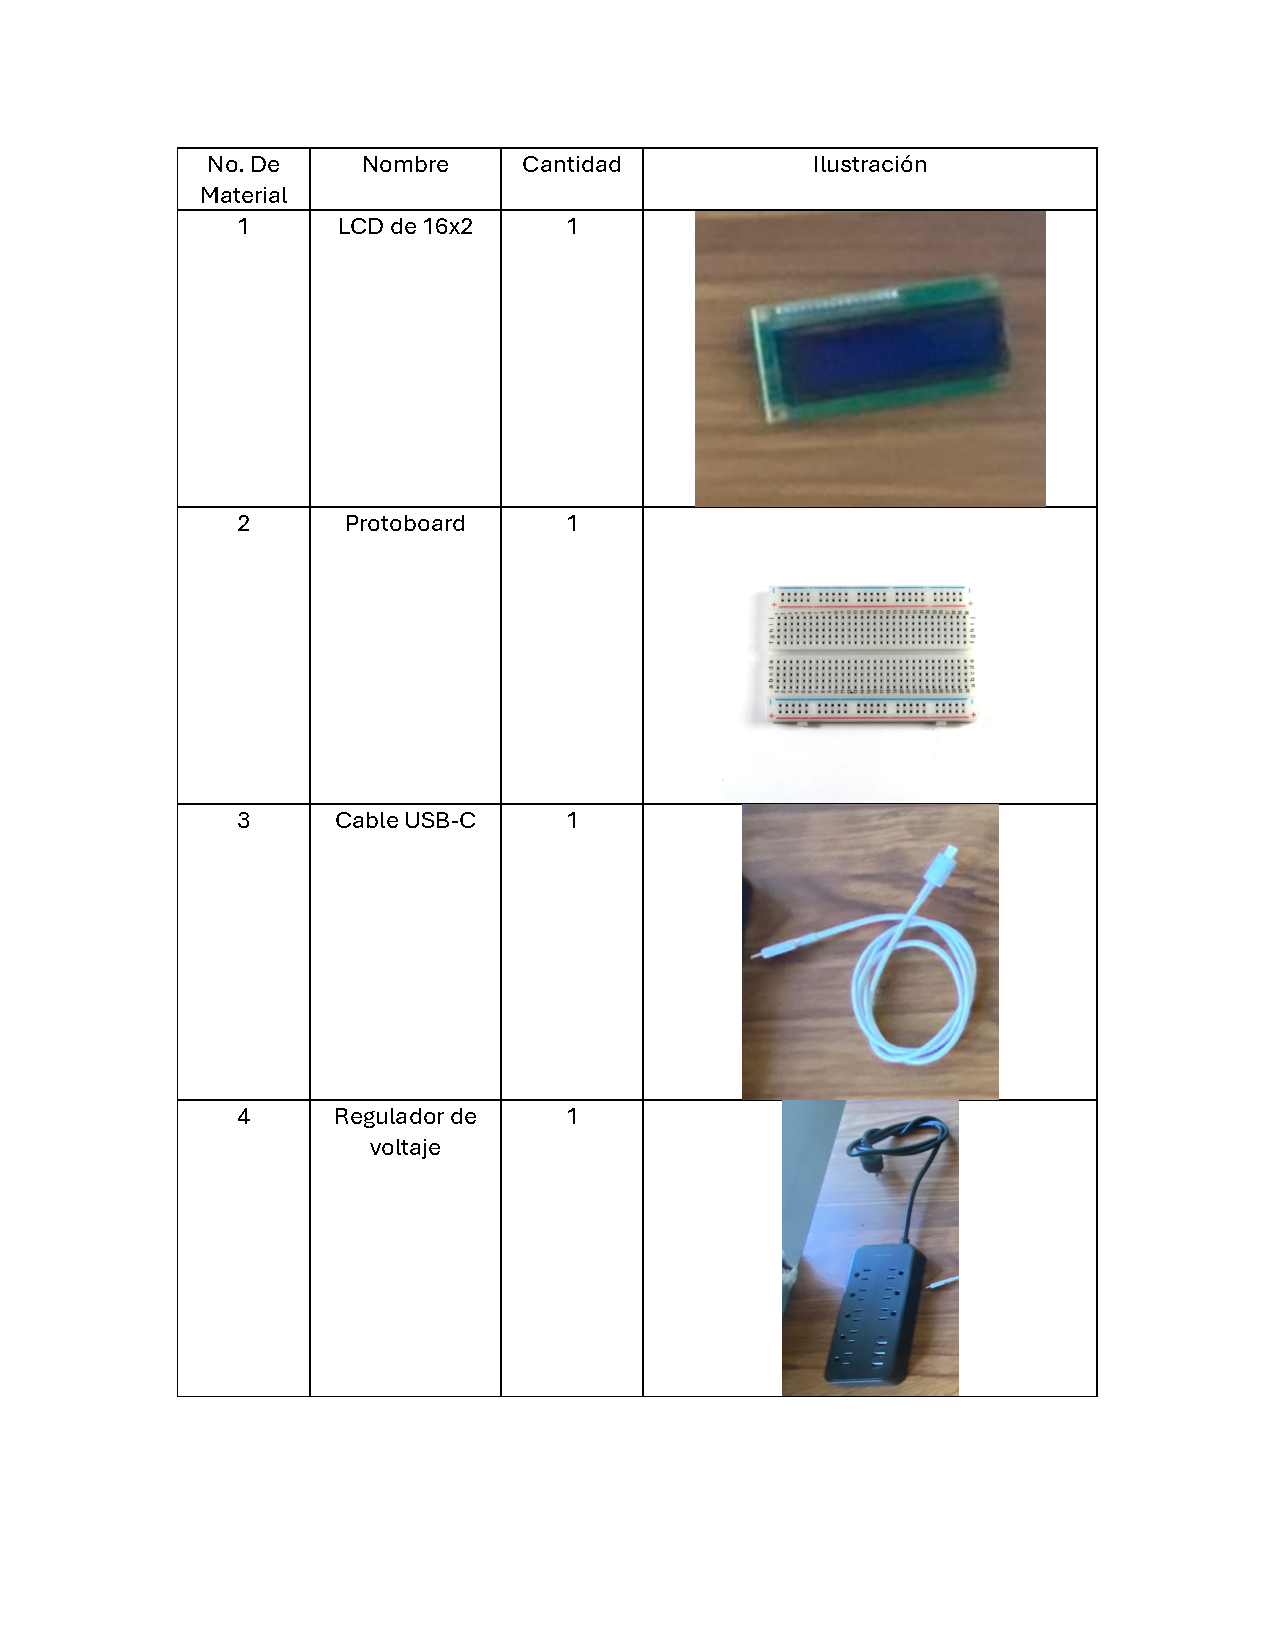
\includegraphics[scale=0.2] {15/img/listaDeMateriales.pdf}
        \caption{Lista de Materiales.}
        \label{fig:listaDeMateriales}
    \end{figure}
    
    \subsubsection{LCD de 16x2}
    Es considerado como un pequeño dispositivo con pantalla de cristal líquido que cuenta con dos filas, de dieciséis caracteres cada una, que se utiliza para mostrar información, por lo general alfanumérica, teniendo como caracterizticas las siguientes: 
    
    \begin{itemize}
    %
        \item Display LCD de 16x2, Pantalla LCD de 16x2.
        \item LCD Alfanumerico.
        \item 5x8 puntos incluye cursor.
        \item Fuente de alimentación de 5V (también disponible para 3V).
        \item Voltaje negativo opcional para alimentación de 3V.
        \item 1/16 duty cycle.
        \item LED puede ser conducido por PIN1, PIN2, PIN15, PIN16 o A y K.
        %\item Interfaz: 6800 (ST7066 IC), opción SPI/I2C (RW1063 IC).
        
    \end{itemize}
    
    \begin{figure}[H]
        \centering
        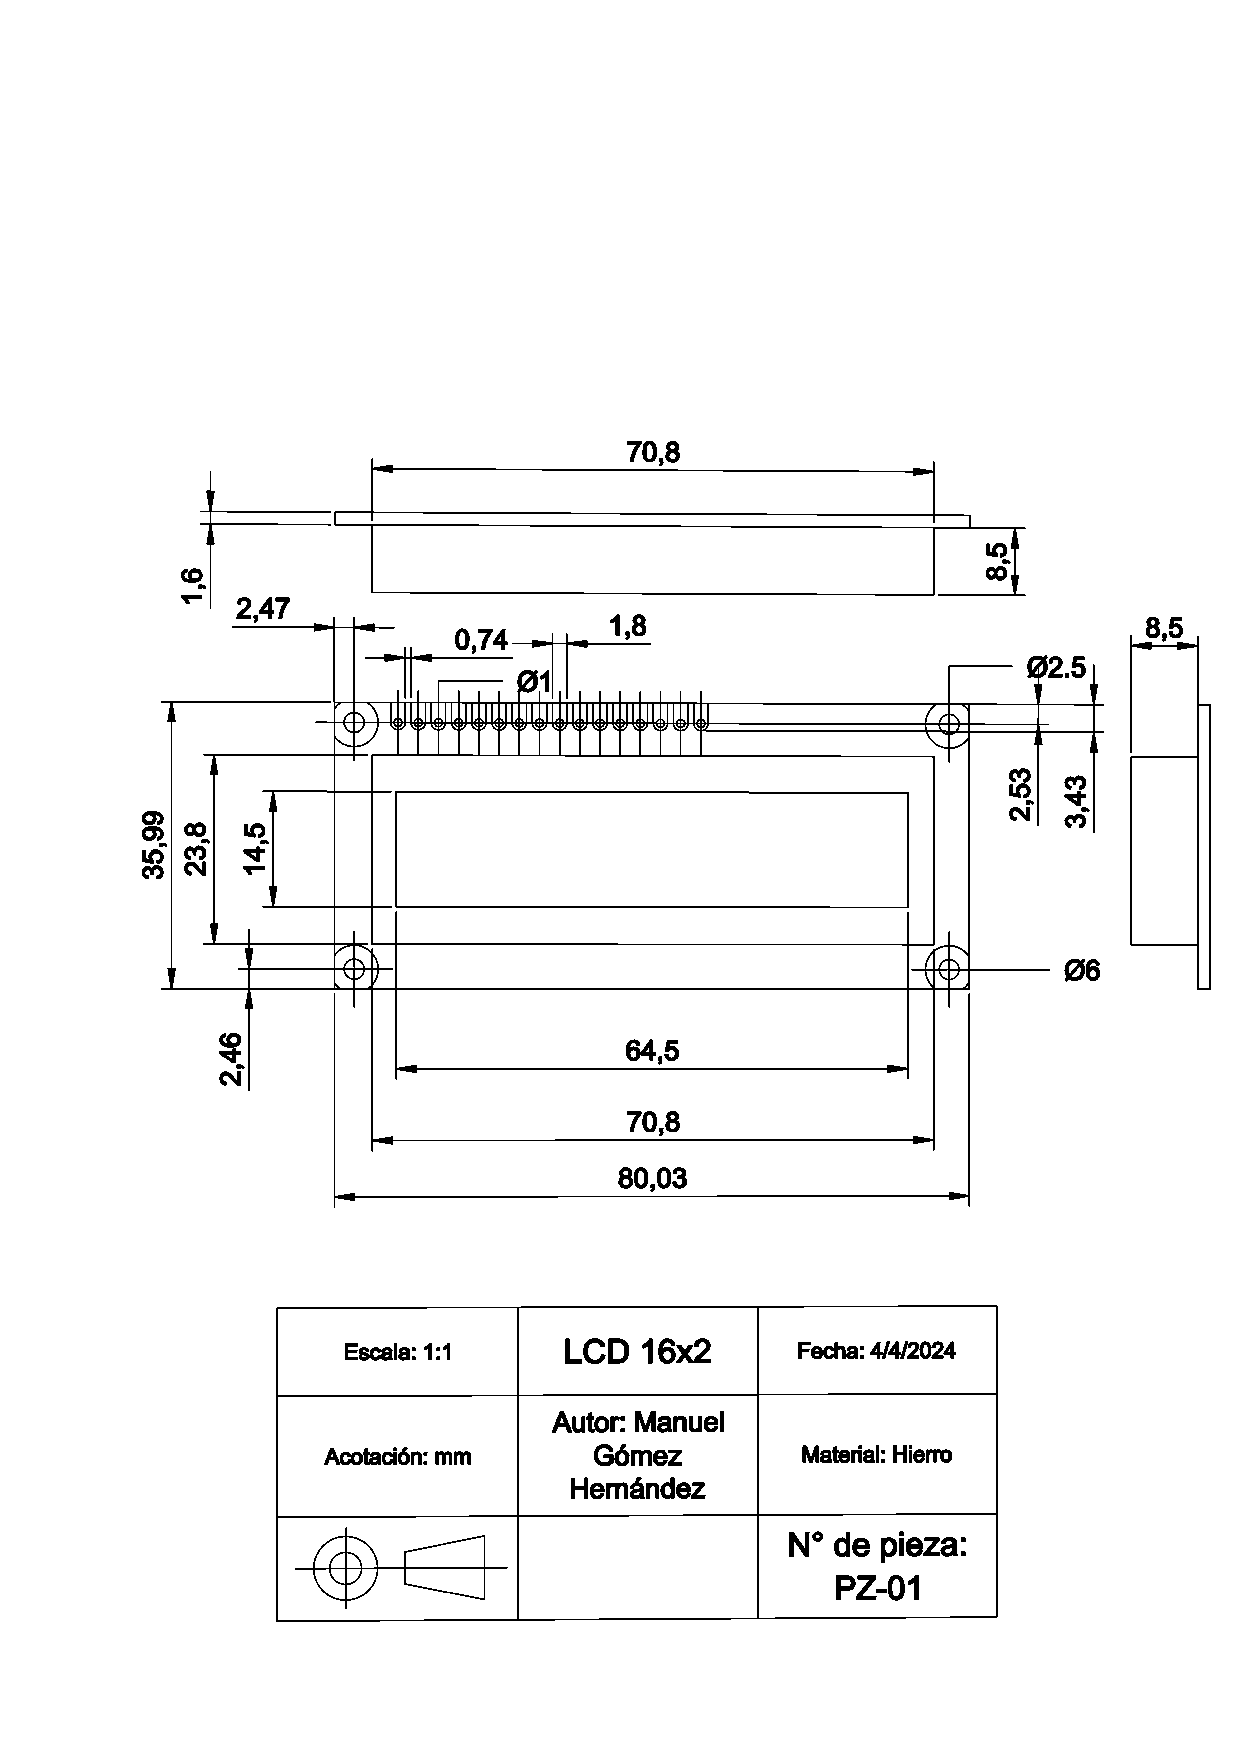
\includegraphics[scale=0.4]{15/img/lcdTrazo.pdf}
        \caption{LCD 16x2 con cotas.}
        \label{fig:lcdTrazo}
    \end{figure}
    
    \begin{figure}[H]
        \centering
        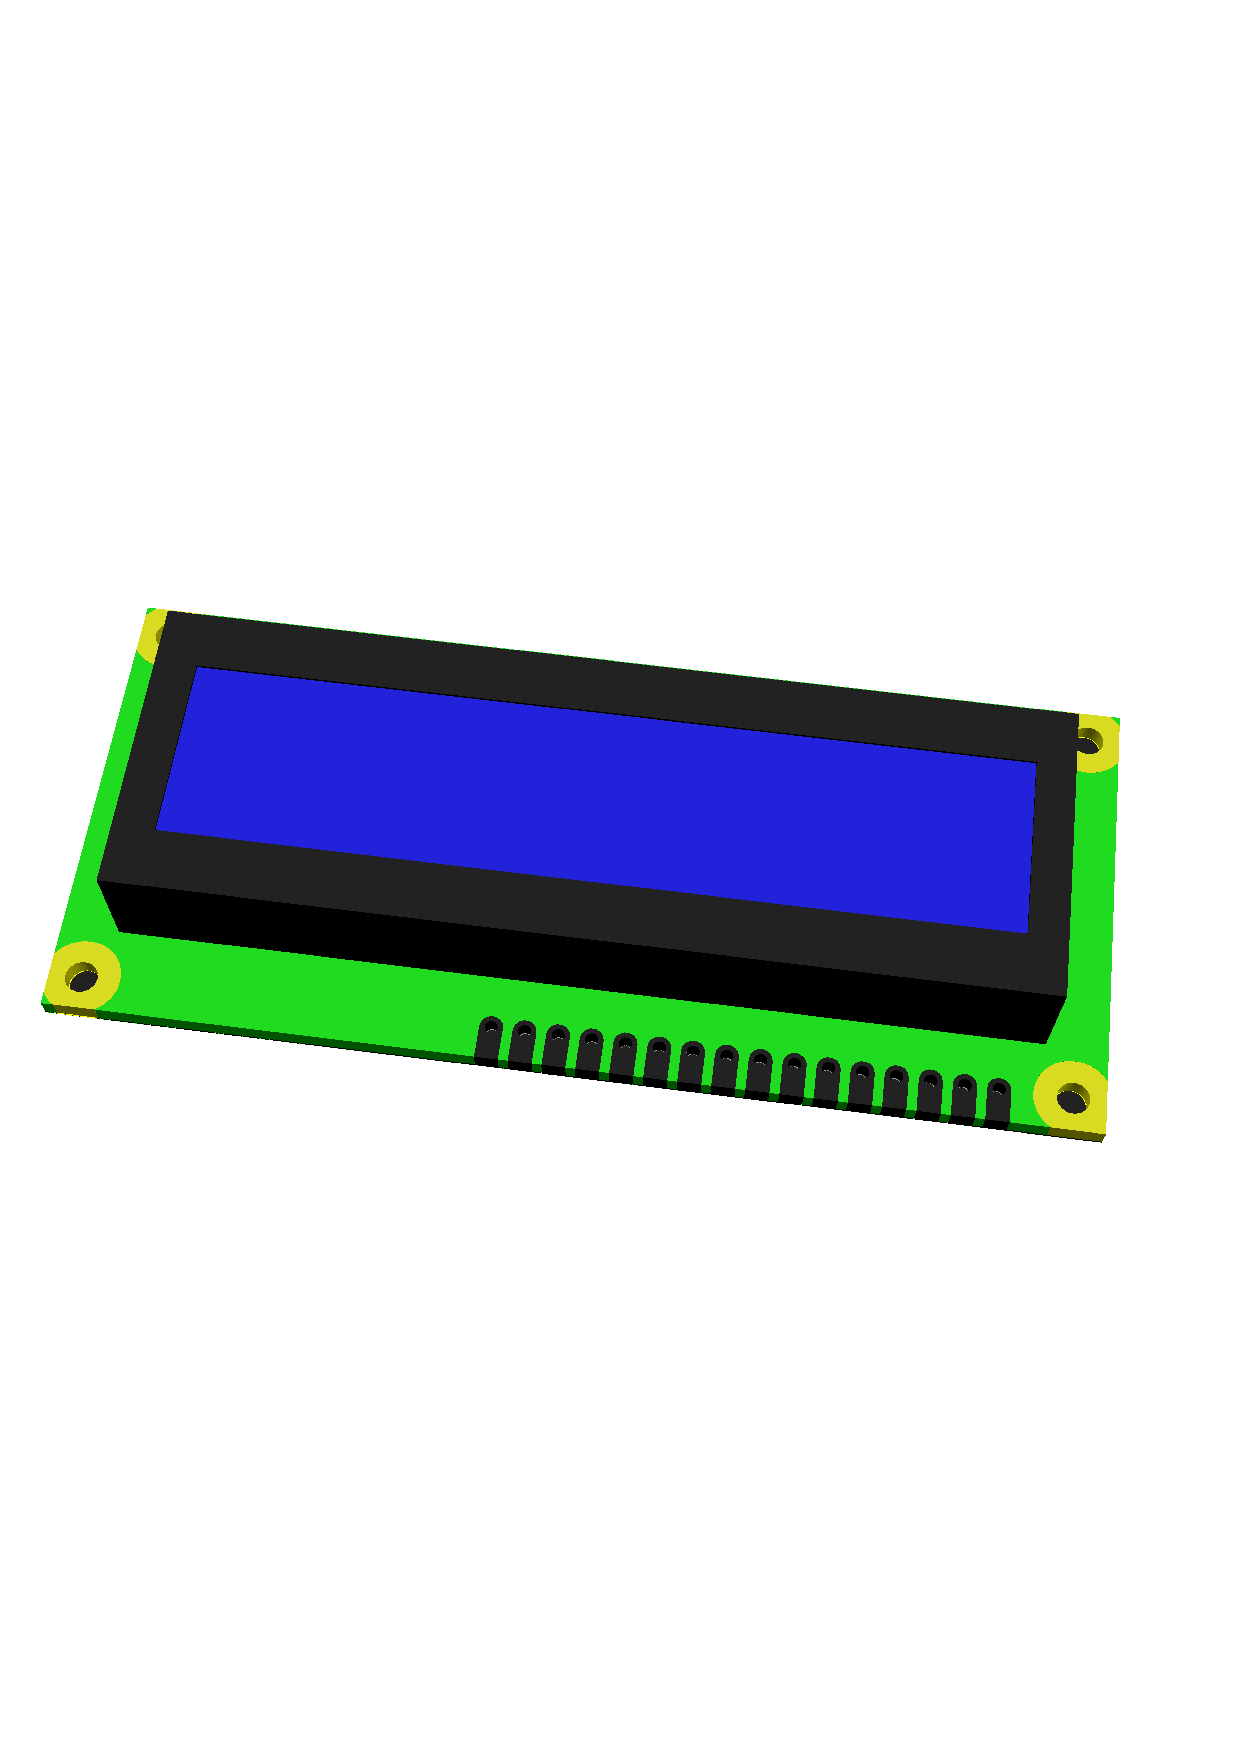
\includegraphics[scale=0.4]{15/img/lcdModelo.pdf}
        \caption{LCD 16x2 en 3D.}
        \label{fig:lcdModelo}
    \end{figure}
    
    \subsubsection{Protoboard 400 puntos}
    La Protoboard, conocida en inglés como breadboard, es una plataforma de pruebas utilizada para ensamblar circuitos electrónicos sin necesidad de soldadura. Esta placa cuenta con orificios interconectados mediante láminas metálicas. Generalmente, los orificios de una misma fila están conectados eléctricamente, mientras que los de diferentes filas no lo están. Los orificios suelen tener una separación estándar de 2.54 mm (0.1 pulgadas) y sus caracterizticas son las siguientes:
    
    \begin{itemize}
        \item Tipo: Protoboard
        \item Puntos: 400 puntos
        \item Color: Transparente
        \item Material: Plástico (ABS)
        \item Longitud: 82 mm
        \item Ancho: 55 mm
        \item Altura: 8.5 mm
        \item Peso de la unidad: 45 g
        \item Voltaje máximo: 36 V
        \item Máxima capacidad de corriente: 3A
        \item Acepta cables con diámetro: 0.4 a 0.7 mm
        \item Autoadherible
    \end{itemize}
    
    \begin{figure}[H]
        \centering
        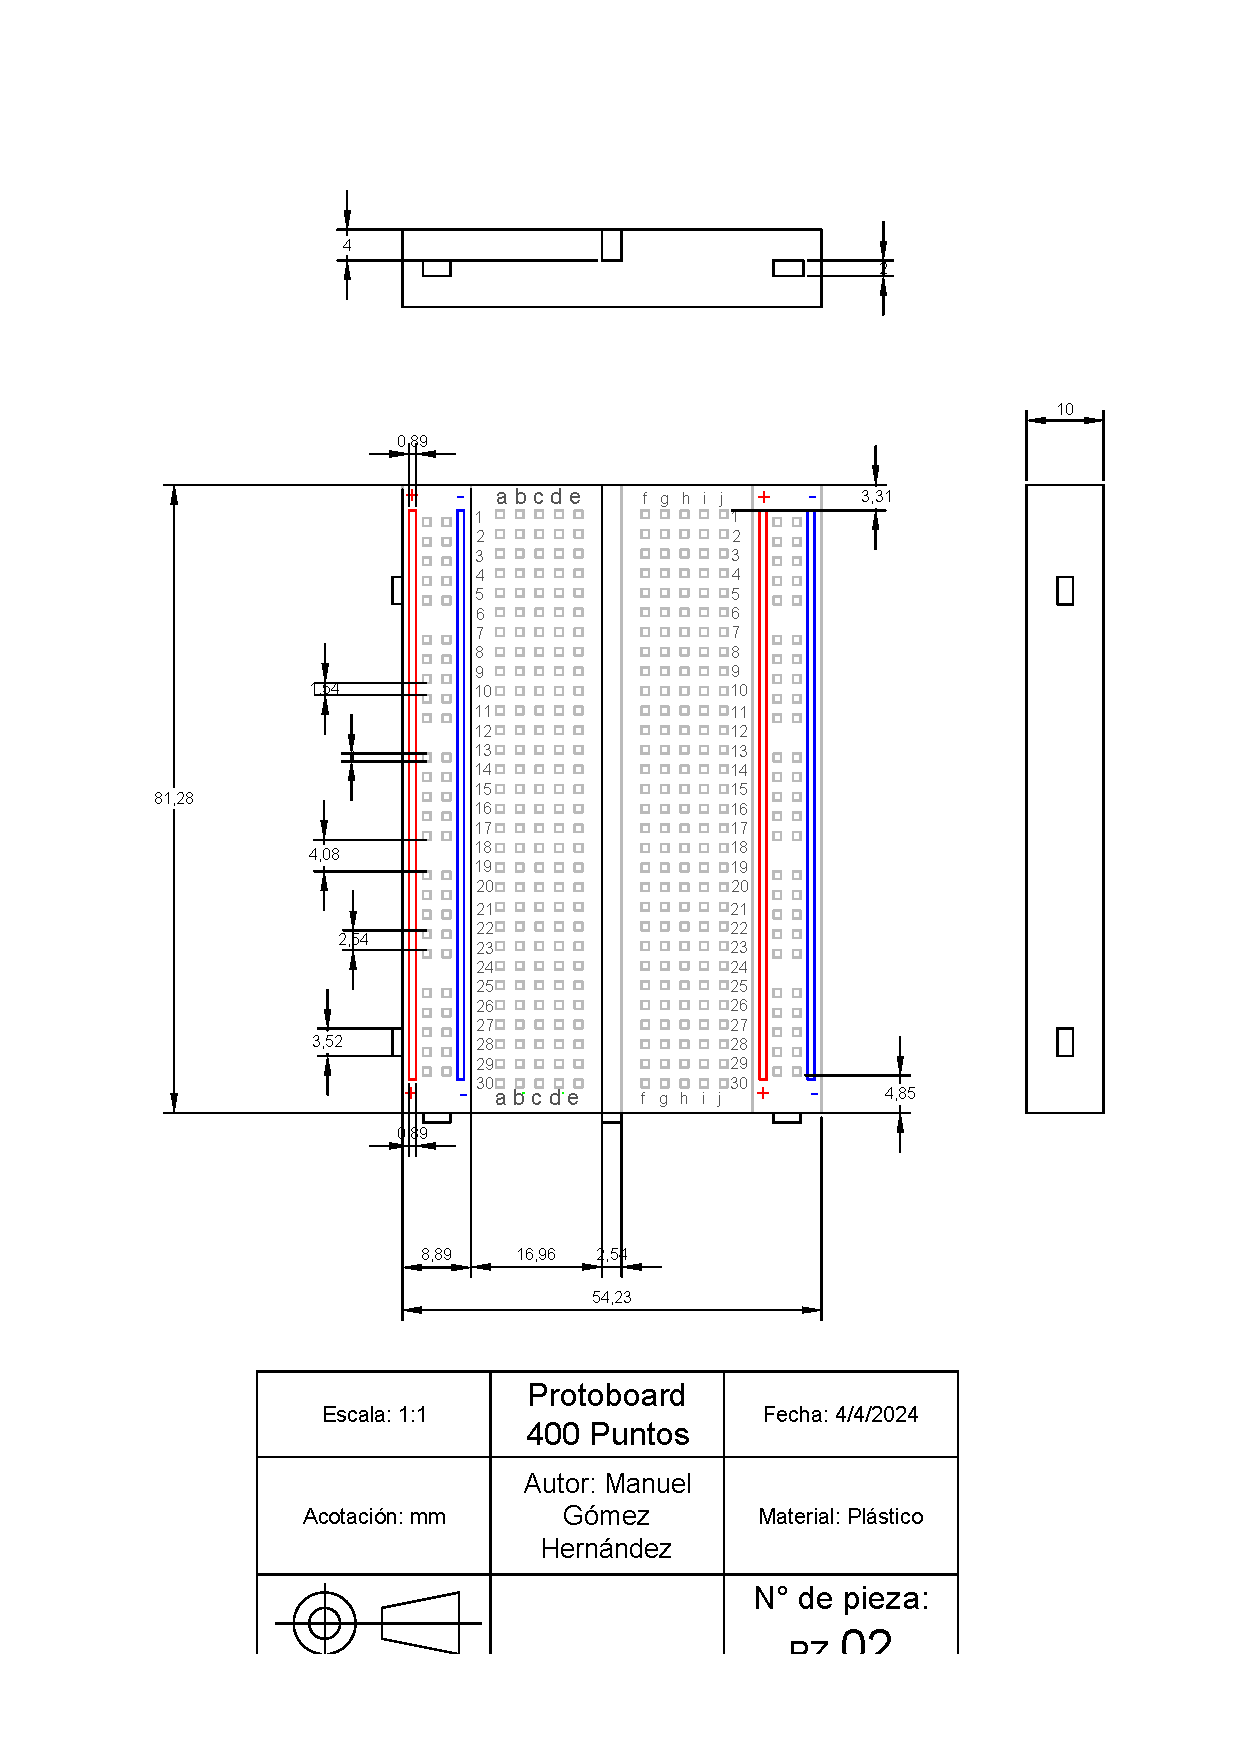
\includegraphics[scale=0.4]{15/img/placaProtoboardTrazo.pdf}
        \caption{Placa Protoboard de 400 puntos con cotas.}
        \label{fig:placaProtoboardTrazo}
    \end{figure}
    
    \begin{figure}[H]
        \centering
        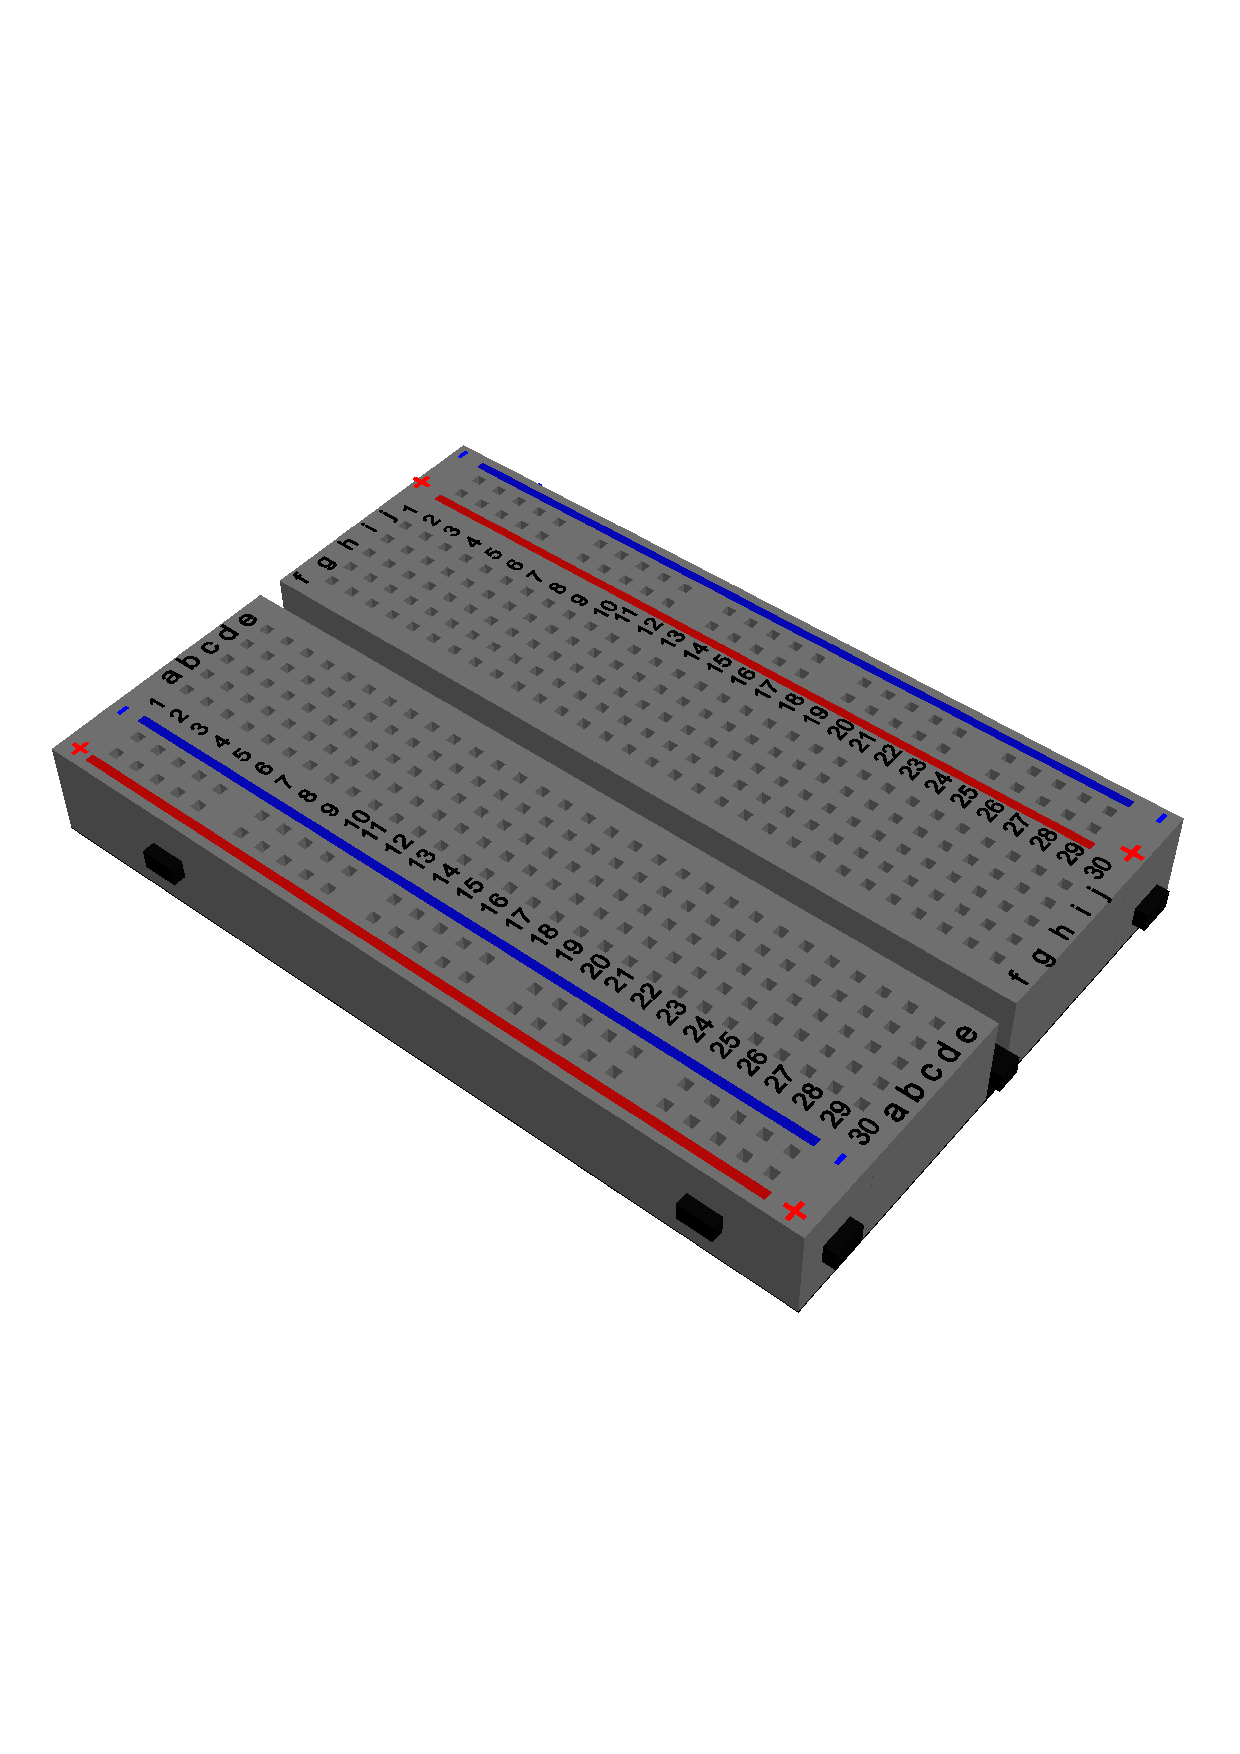
\includegraphics[scale=0.4]{15/img/placaProtoboardModelo.pdf}
        \caption{Placa Protoboard de 400 puntos en 3D.}
        \label{fig:placaProtoboardModelo}
    \end{figure}
    
    \subsubsection{Cable USB-C}
    
    
    
    %\begin{figure}[H]
     %   \centering
      %  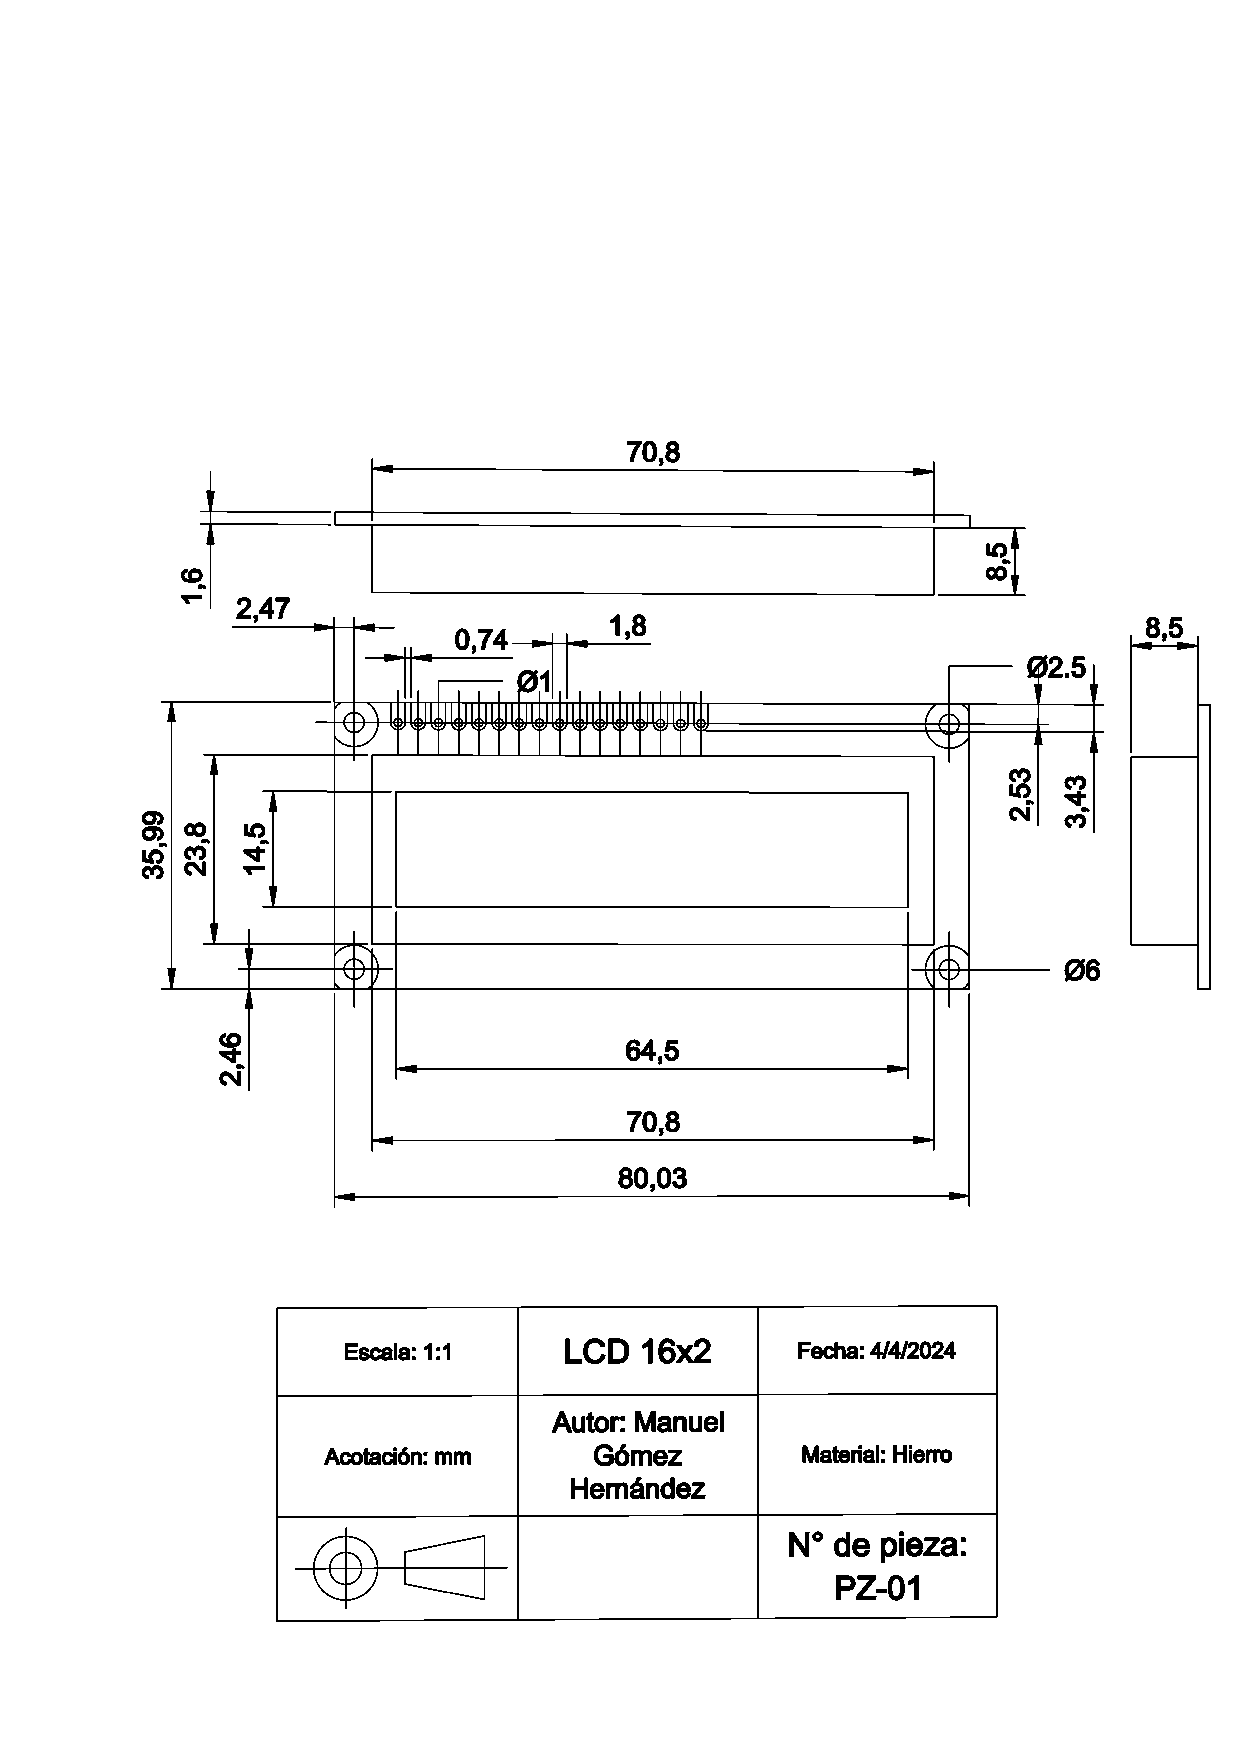
\includegraphics[scale=0.4]{15/img/lcdTrazo.pdf}
       % \caption{LCD 16x2.}
        %\label{fig:lcdTrazo}
    %\end{figure}
    
    \subsubsection{Modulo SPI I2c}
    
    
    %\begin{figure}[H]
     %   \centering
      %  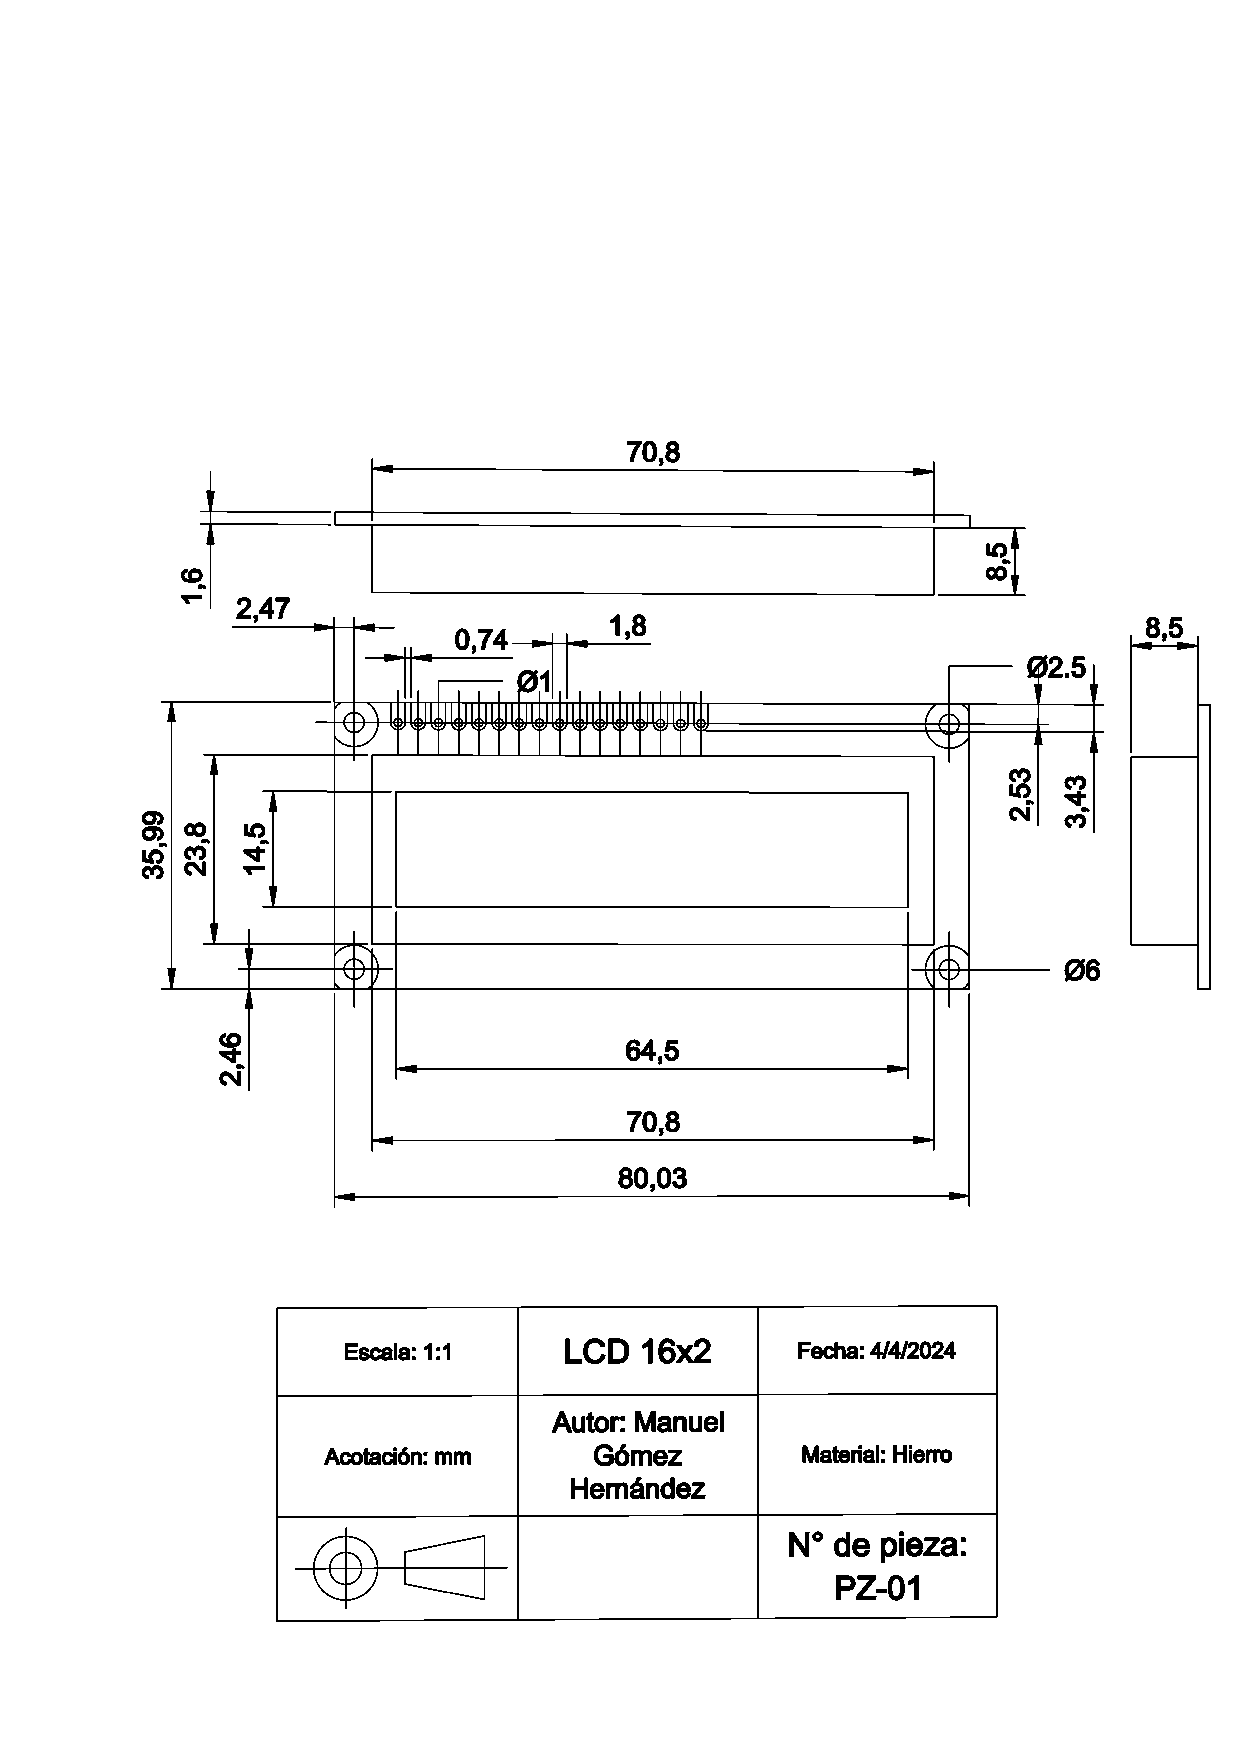
\includegraphics[scale=0.4]{15/img/lcdTrazo.pdf}
       % \caption{LCD 16x2.}
        %\label{fig:lcdTrazo}
    %\end{figure}
    
    \subsubsection{ESP32-C6}
    El ESP32-C6-DevKit Placa de Desarrollo Dual Tipo C es una placa de desarrollo basada en el microcontrolador ESP32-C6 de Espressif Systems, una versión actualizada de la serie ESP32 que ofrece capacidades mejoradas de conectividad Wi-Fi y Bluetooth de baja energía (BLE). Esta placa de desarrollo ofrece un entorno para probar, desarrollar y crear aplicaciones y dispositivos IoT (Internet de las cosas) con estas funcionalidades mejoradas.
    
    El ESP32-C6-DevKit Placa de Desarrollo Dual Tipo C puede ser utilizado para una amplia gama de aplicaciones IoT, desde sistemas de monitoreo remoto hasta dispositivos conectados en el hogar, soluciones industriales y más, gracias a sus capacidades mejoradas de conectividad.
    
    Caracterizticas y especificaciones: 
    \begin{itemize}
        \item CPU: ESP32-C6
    \item Memoria
    FLASH: 4MB
    ROM:320 KB
    HP SRAM: 512 KB
    LP SRAM: 16KB
    \item Funciona en banda de frecuencia de 2.4 GHz, 1T1R
    \item Compatible con Bluetooth Low Energy 5,0
    \item Admite el protocolo IEEE 802.11ax,
    \item Compatible con protocolos IEEE 802.11b/G/n, compatible con ancho de banda de 20 MHz y 40 MHz-velocidades de datos de hasta 150 Mbps
    \item Forma de antena: Antena PCB integrada
    \item Temperatura de funcionamiento:-40 ℃ ~ 85 ℃
    \item Puertos
    GPIO: 32
    SPI: 3
    UART: 2
    I2C: 1
    ADC: 1
    \end{itemize}
    
    
    \begin{figure}[H]
        \centering
        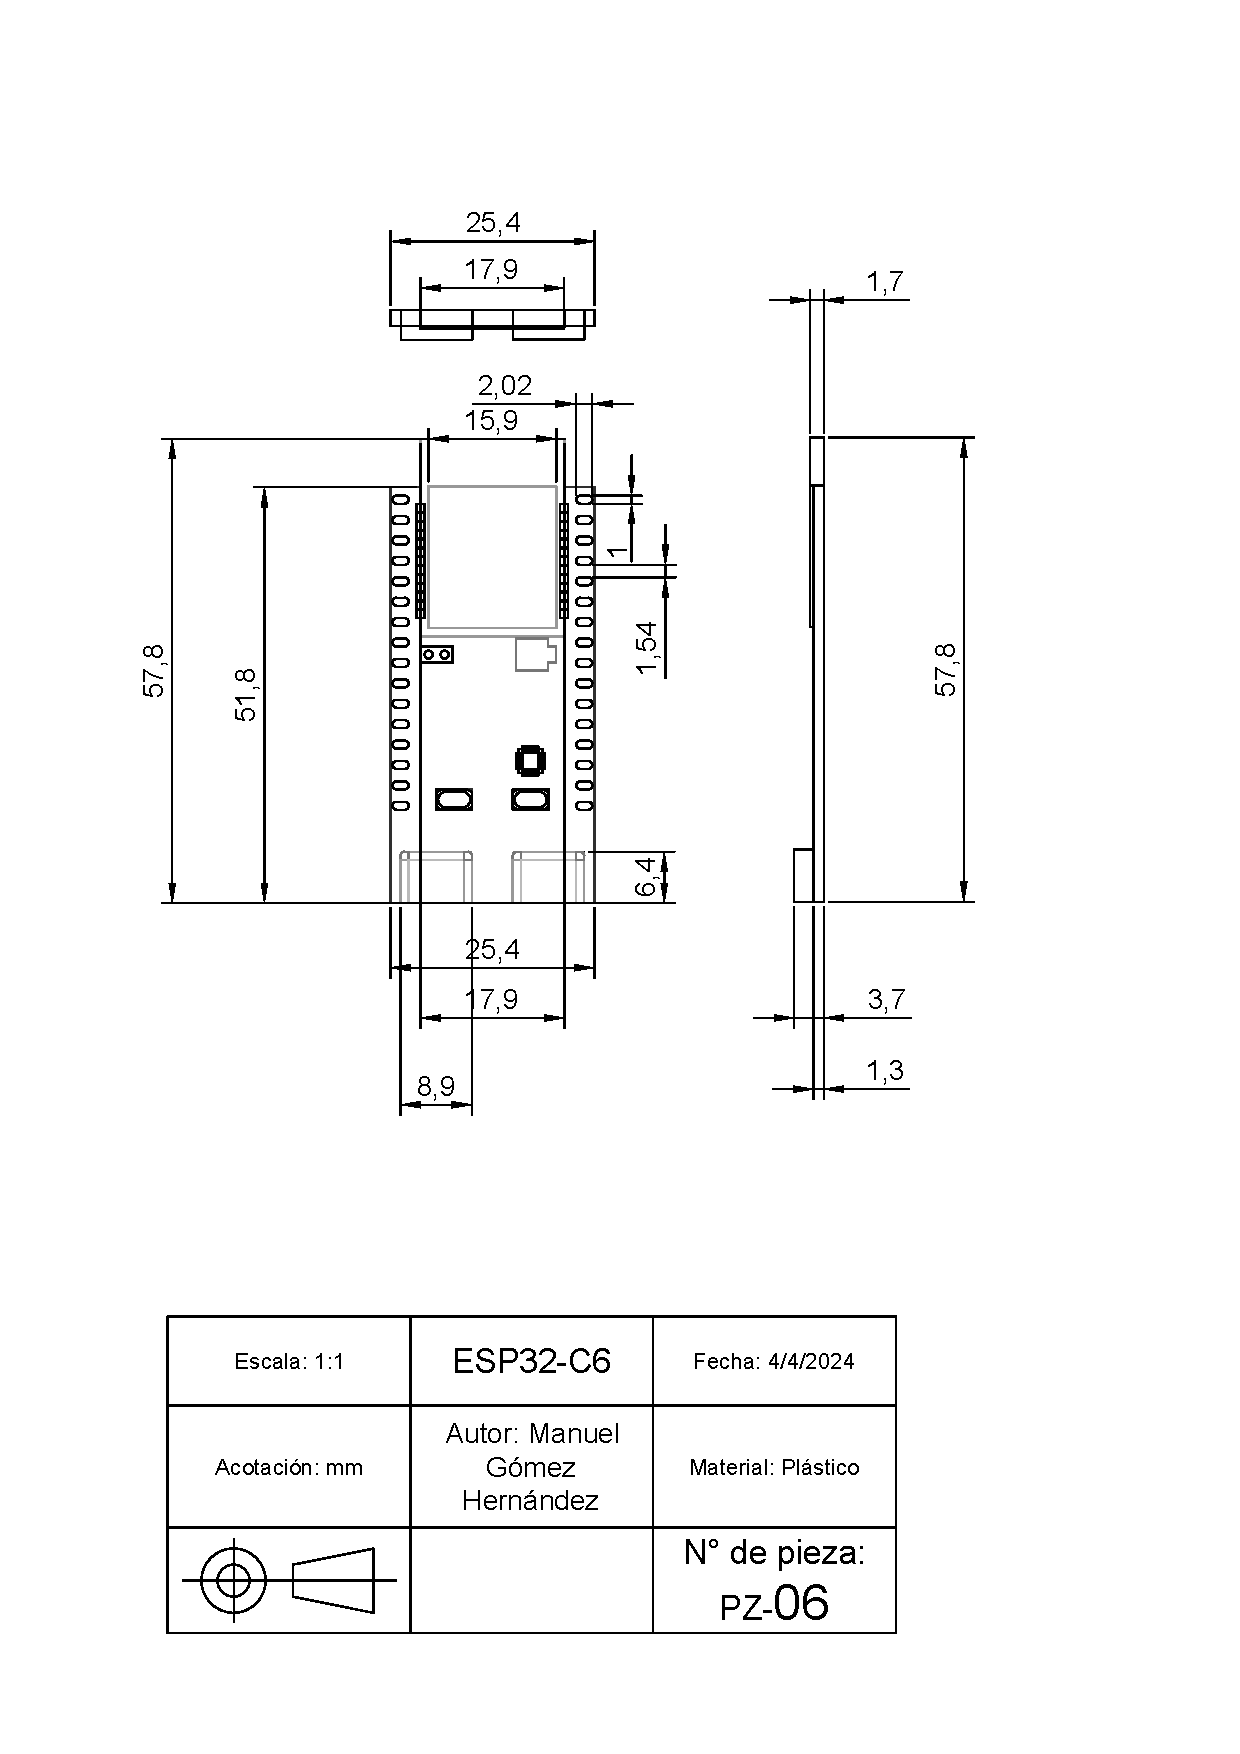
\includegraphics[scale=0.4]{15/img/eSP32Trazo.pdf}
        \caption{ESP32-C6 con cotas.}
        \label{fig:eSP332Trazo}
    \end{figure}
    
    \begin{figure}[H]
        \centering
        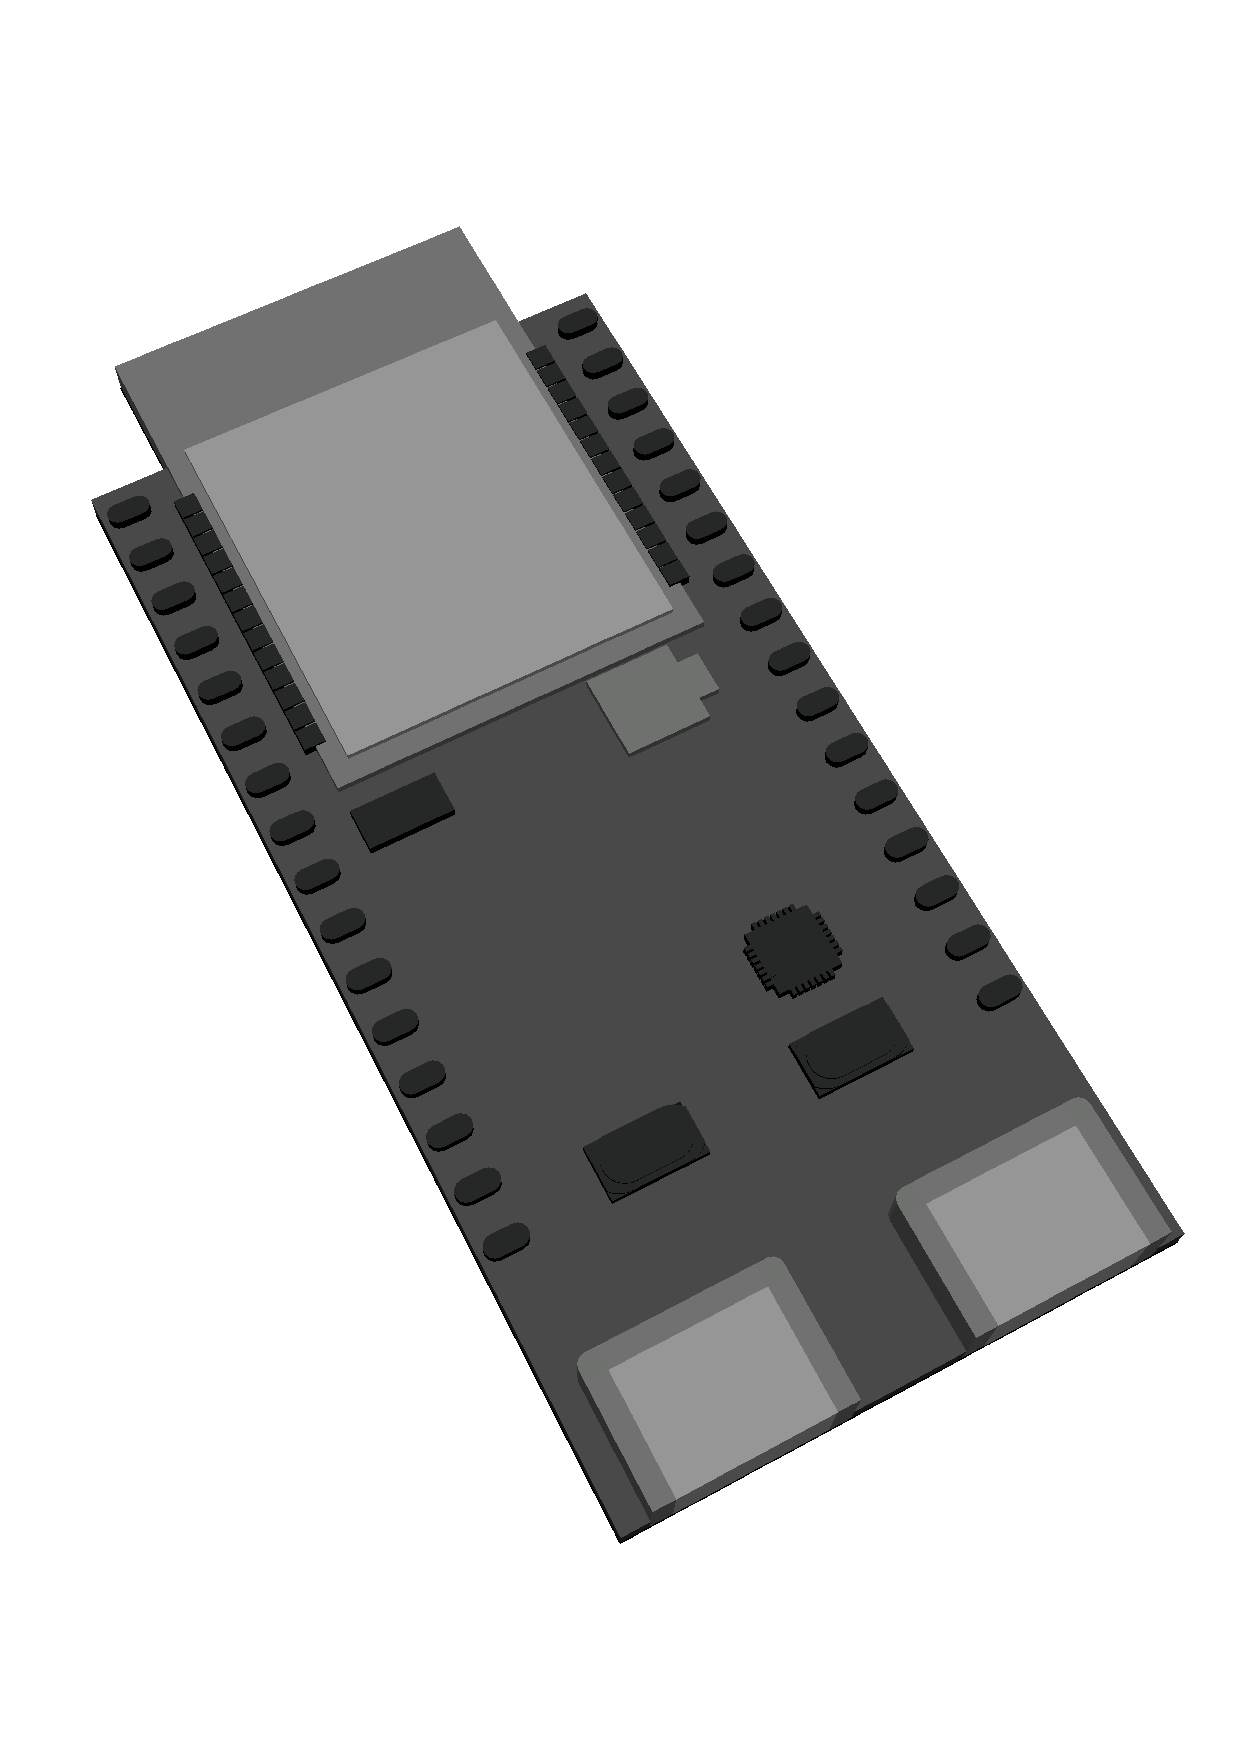
\includegraphics[scale=0.4]{15/img/eSP32Modelo.pdf}
        \caption{ESP32-C6 en 3D.}
        \label{fig:eSP332Modelo}
    \end{figure}
    
    \subsubsection{Resistencias Th 1K ohm 1W}
    
    La resistencia es la oposición al flujo de corriente eléctrica a través de un conductor. La unidad de resistencia en el Sistema Internacional es el ohmio, en honor al físico alemán Georg Simon Ohm, quien formuló la ley que lleva su nombre.
    
    En un circuito eléctrico, la resistencia tiene la función de oponerse al flujo de la corriente eléctrica, reduciendo la intensidad de corriente circulante. El valor de una resistencia se puede determinar mediante el código de colores \ref{fig:codigoColoresResistencia}. 
    
    Las resistencias de montaje en superficie vienen en tamaños estándar y son ideales para fabricar placas de circuitos en forma masiva, o en diseños donde el espacio es reducido, en la siguiente imagen podrás ver las cotas de la resistencia utilizada \ref{fig:resistenciaTrazo}, así como su figura 3D \ref{fig:resistenciaModelo}.
    
    \begin{figure}[H]
        \centering
        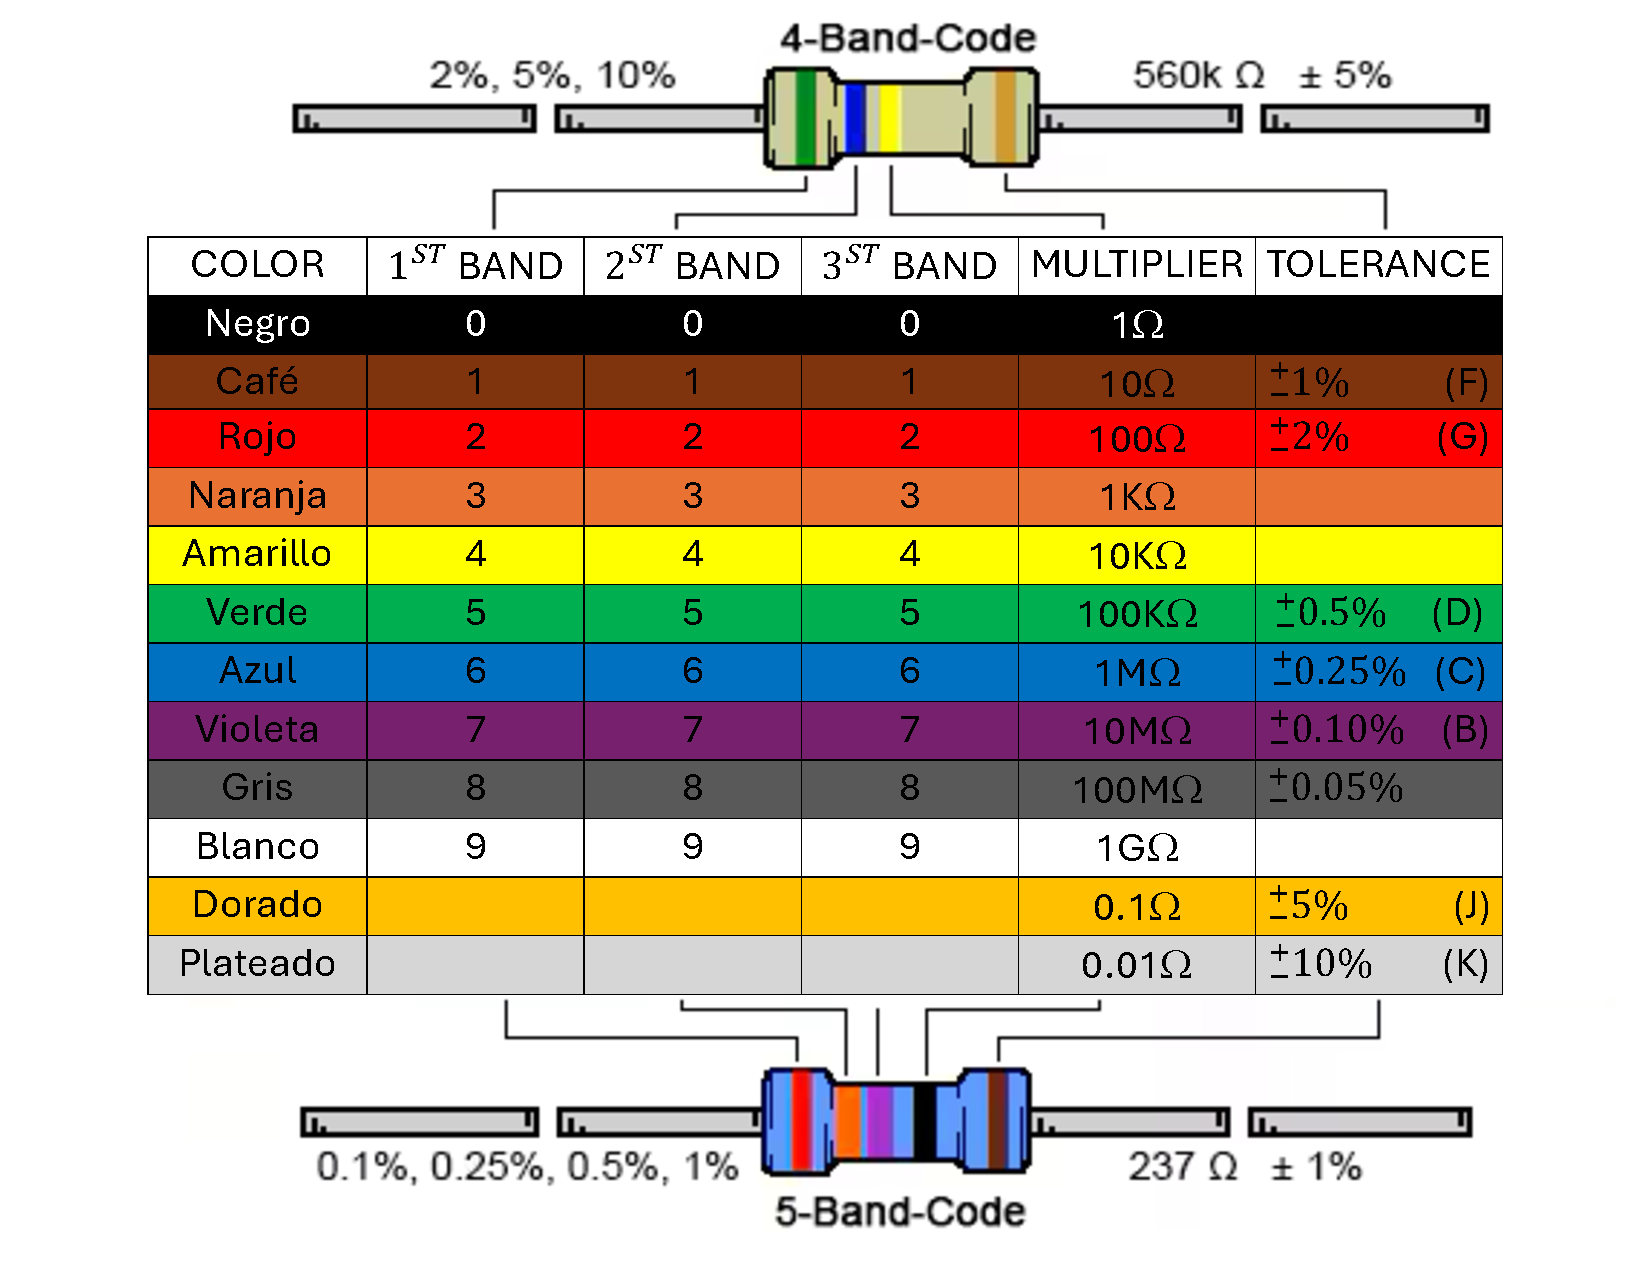
\includegraphics[scale=0.35]{15/img/codigoColoresResistencia.pdf}
        \caption{Código de colores de resistencias.}
        \label{fig:codigoColoresResistencia}
    \end{figure}
         
    
    \begin{figure}[H]
        \centering
        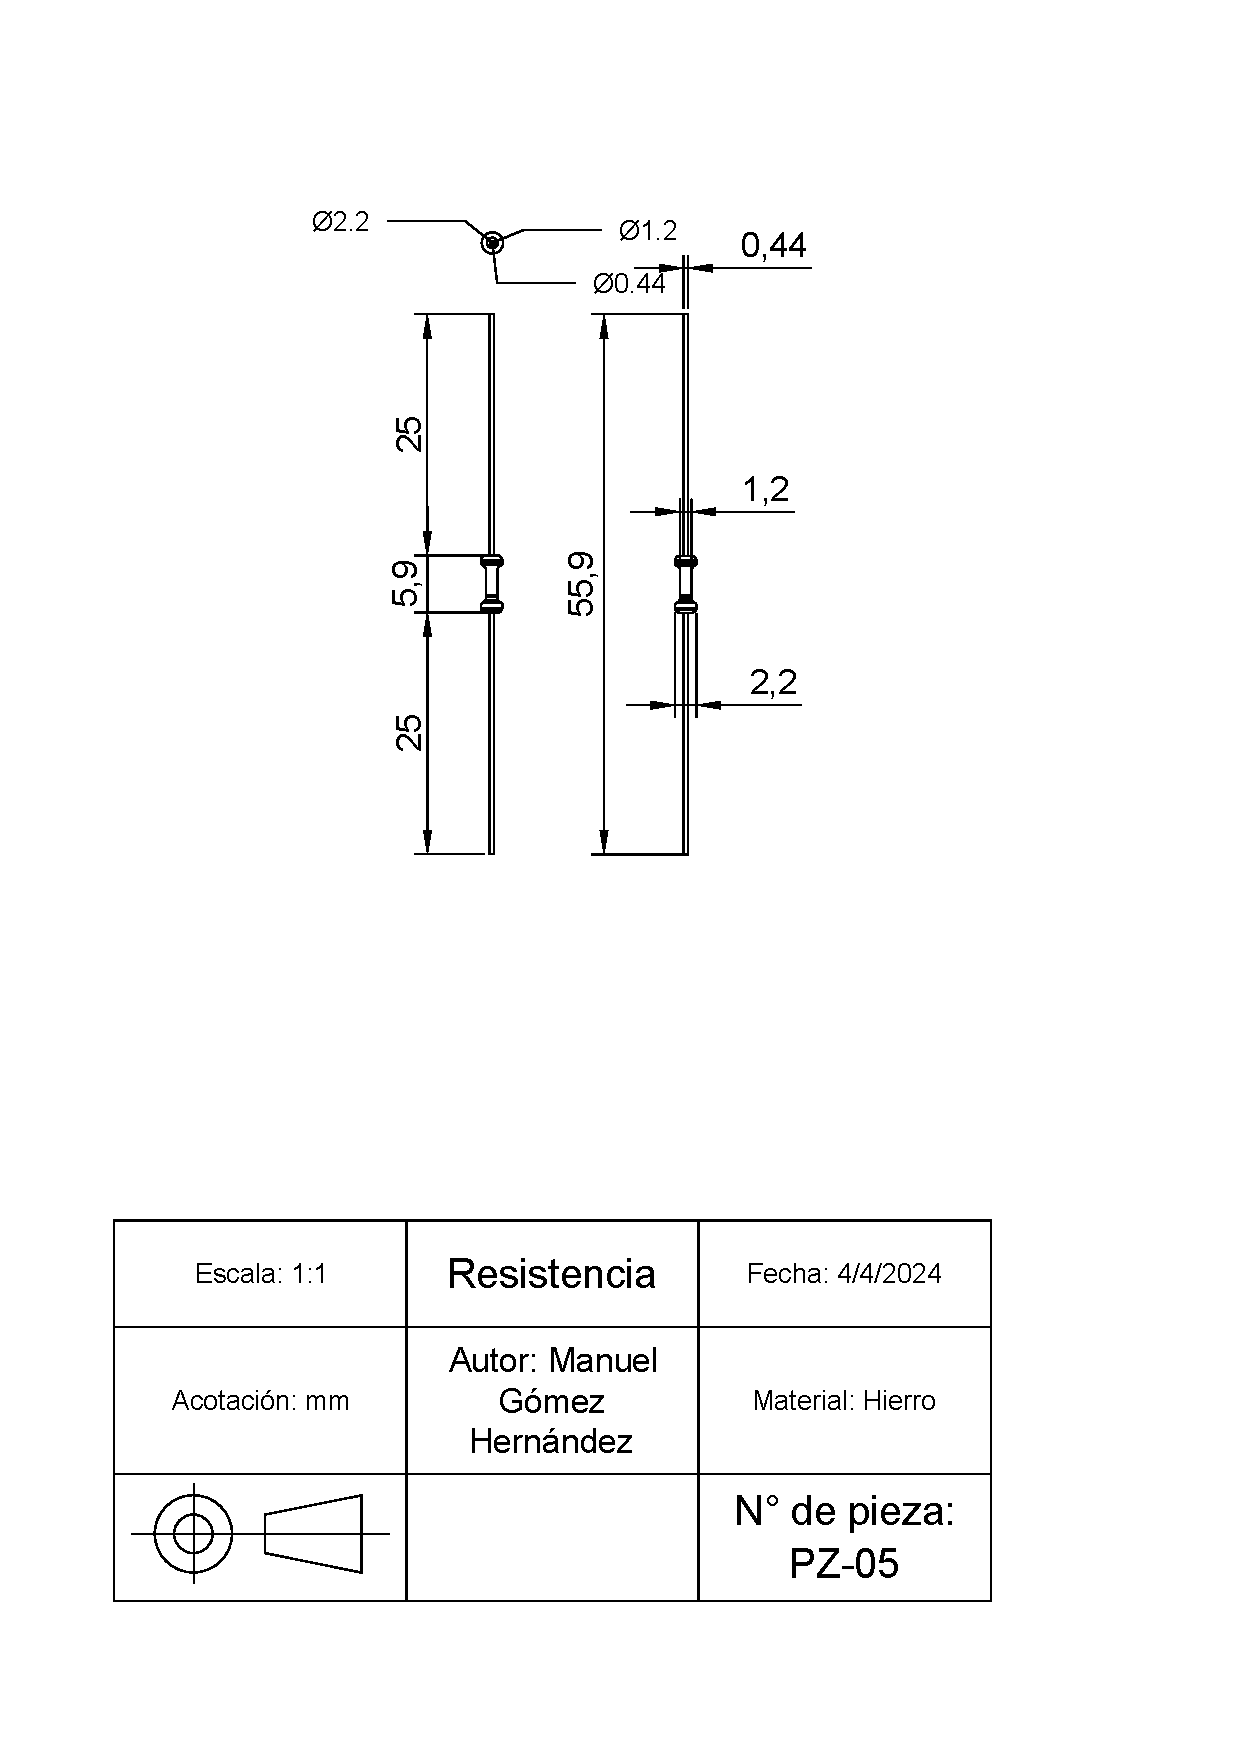
\includegraphics[scale=0.4]{15/img/resistenciaTrazo.pdf}
        \caption{Resistencia con cotas.}
        \label{fig:resistenciaTrazo}
    \end{figure}
    
    \begin{figure}[H]
        \centering
        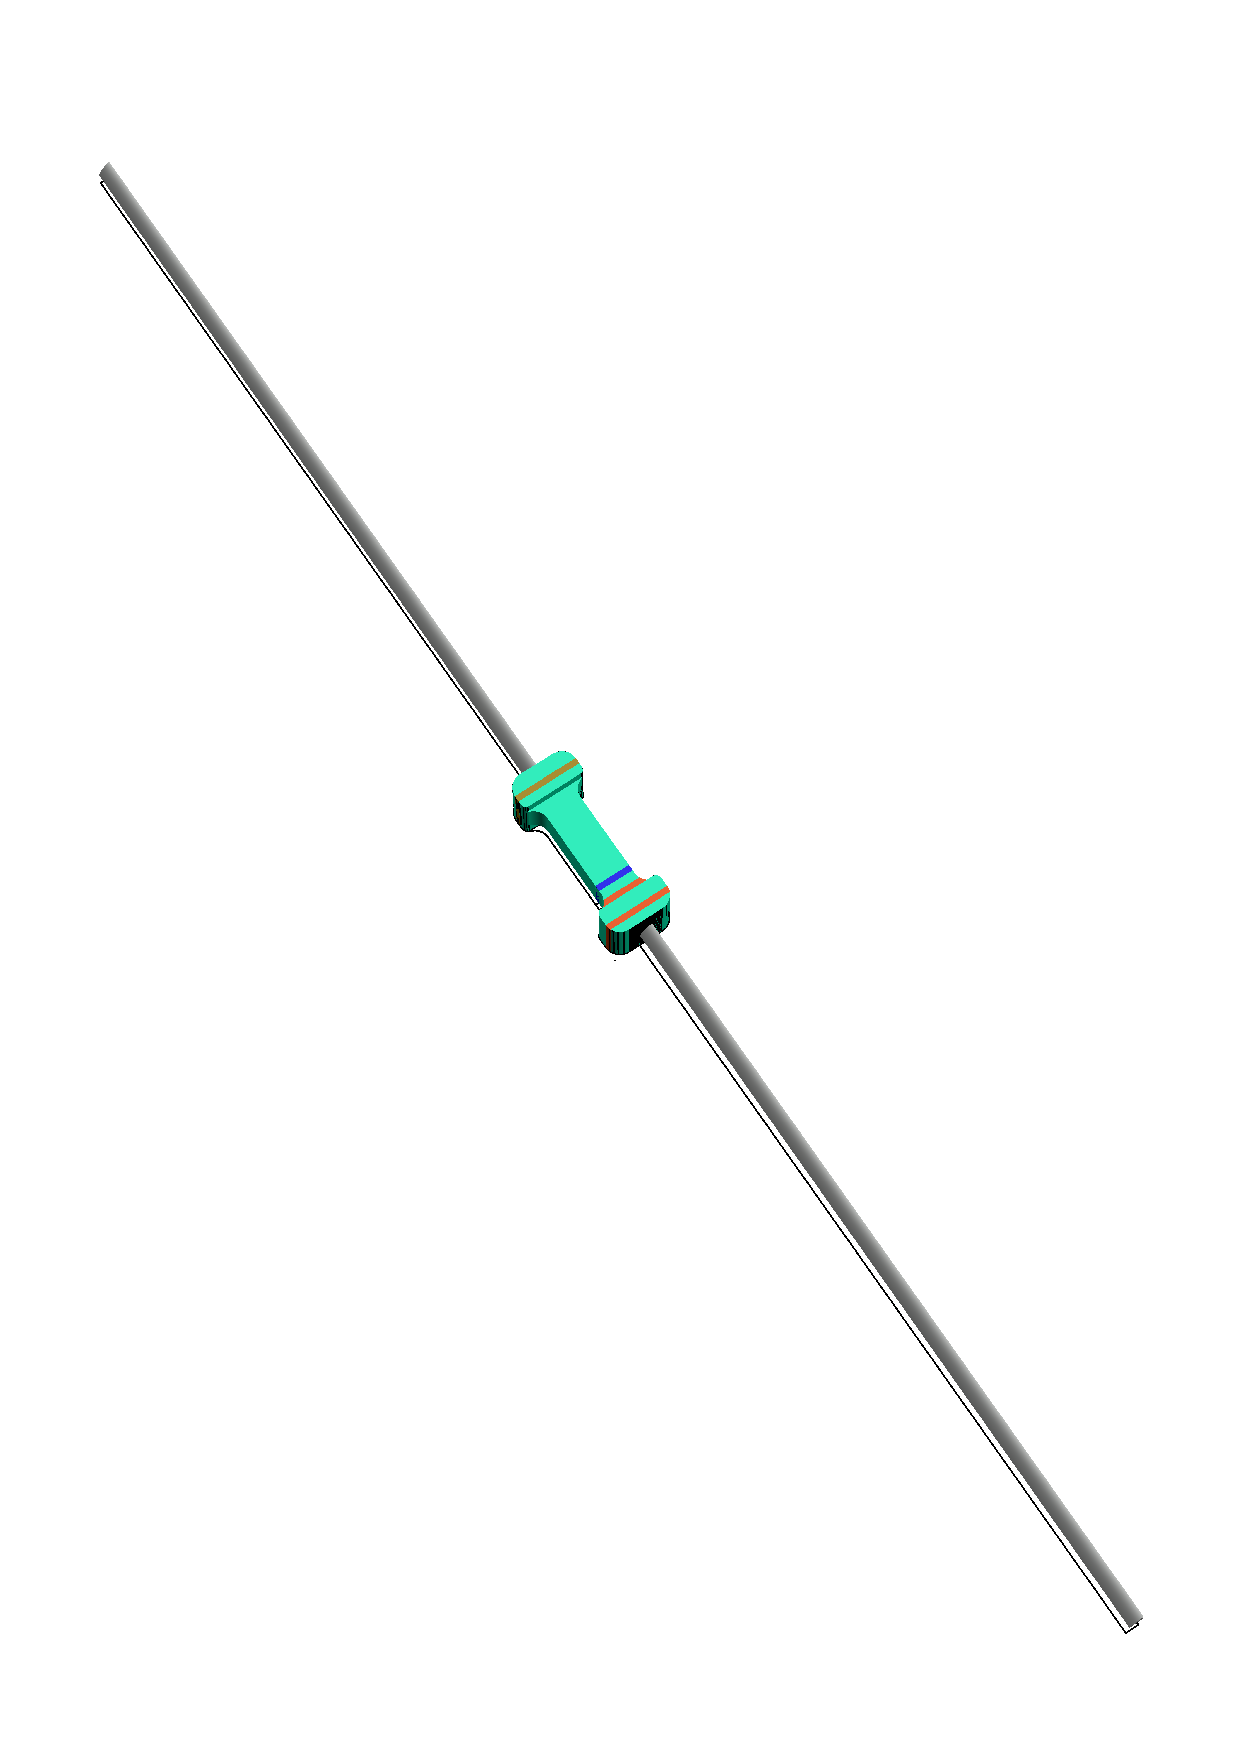
\includegraphics[scale=0.4]{15/img/resistenciaModelo.pdf}
        \caption{Resistencia en 3D.}
        \label{fig:resistenciaModelo}
    \end{figure}
    
    \subsubsection{Cable Jumper Dupont Macho-Hembra 10cm}
    
    
    \begin{figure}[H]
        \centering
        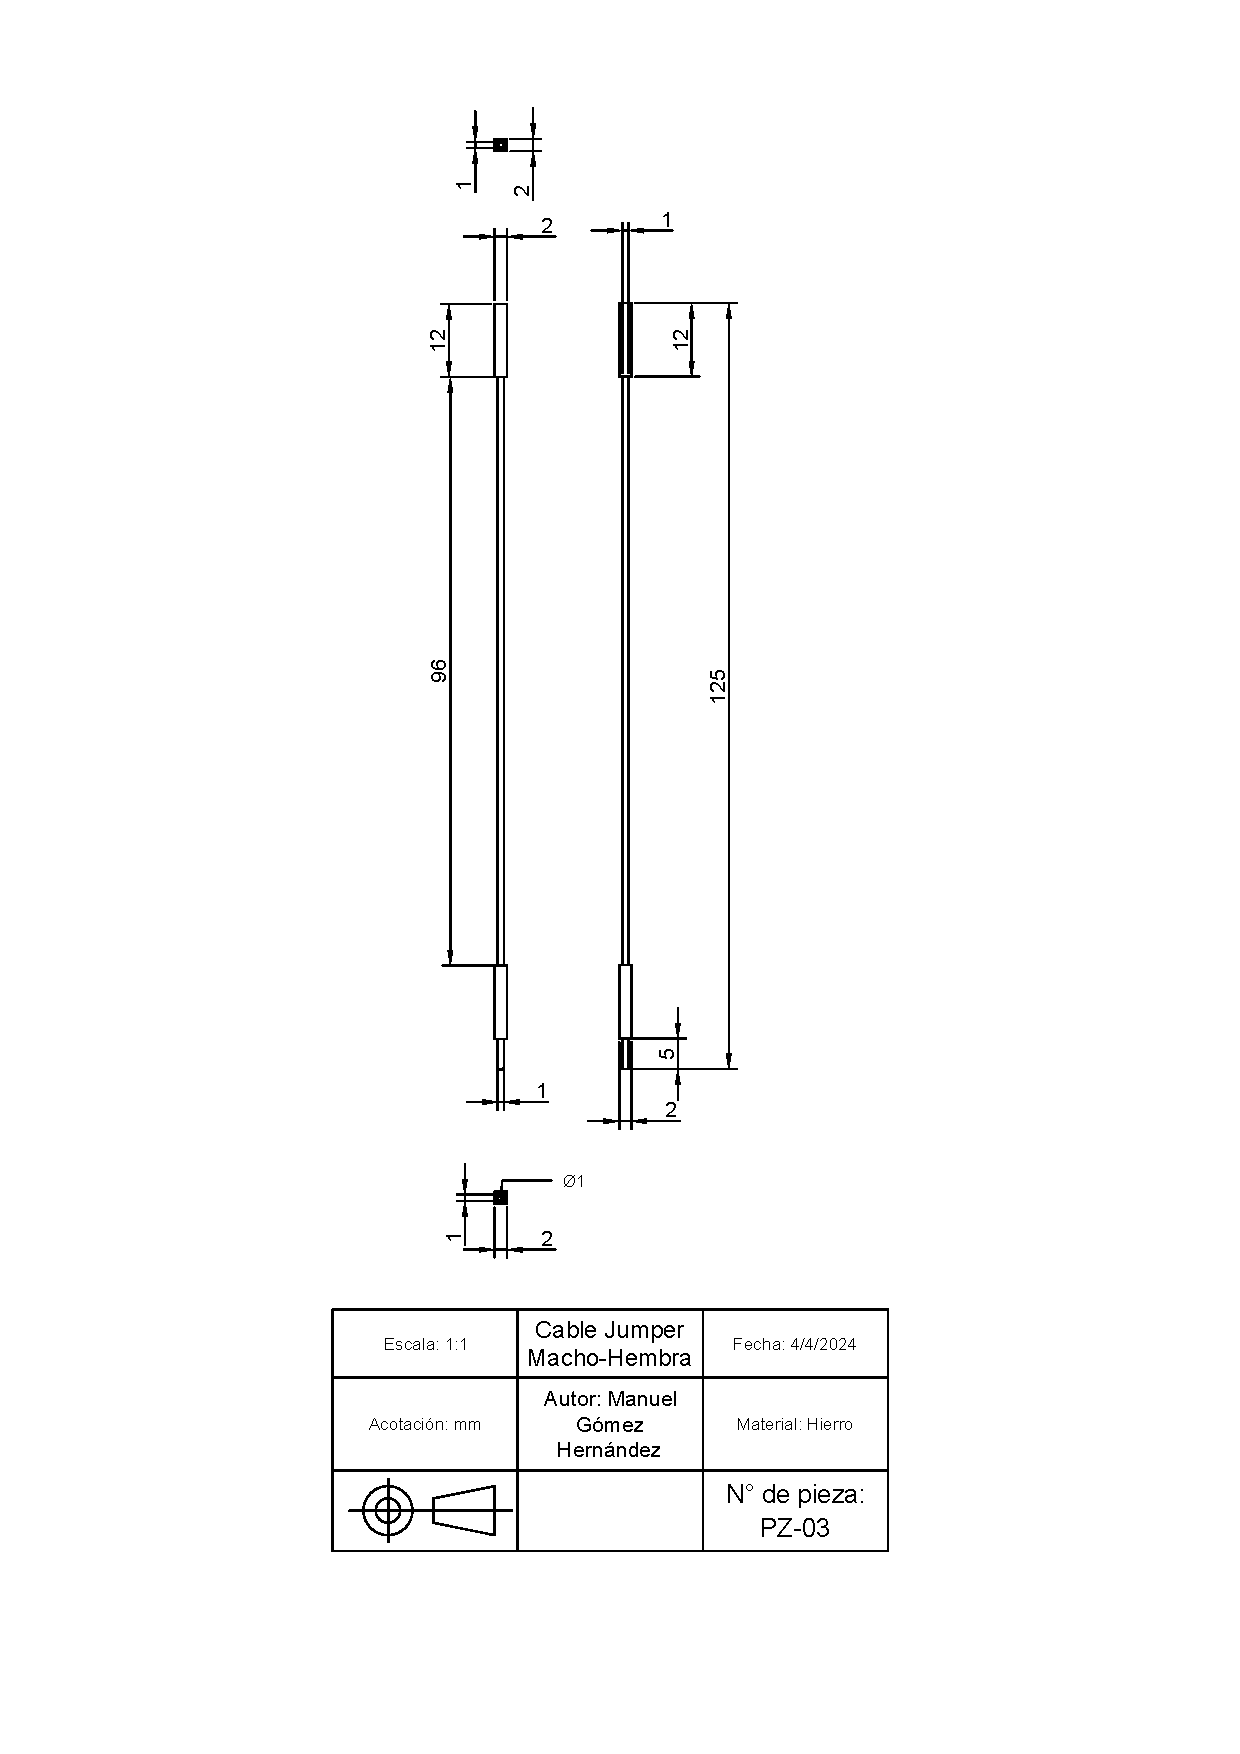
\includegraphics[scale=0.4]{15/img/cableJumperMHTrazo.pdf}
        \caption{Cable Jumper Dupont Macho-Hembra 10cm con cotas.}
        \label{fig:cableJumperMHTrazo}
    \end{figure}
    
    \begin{figure}[H]
        \centering
        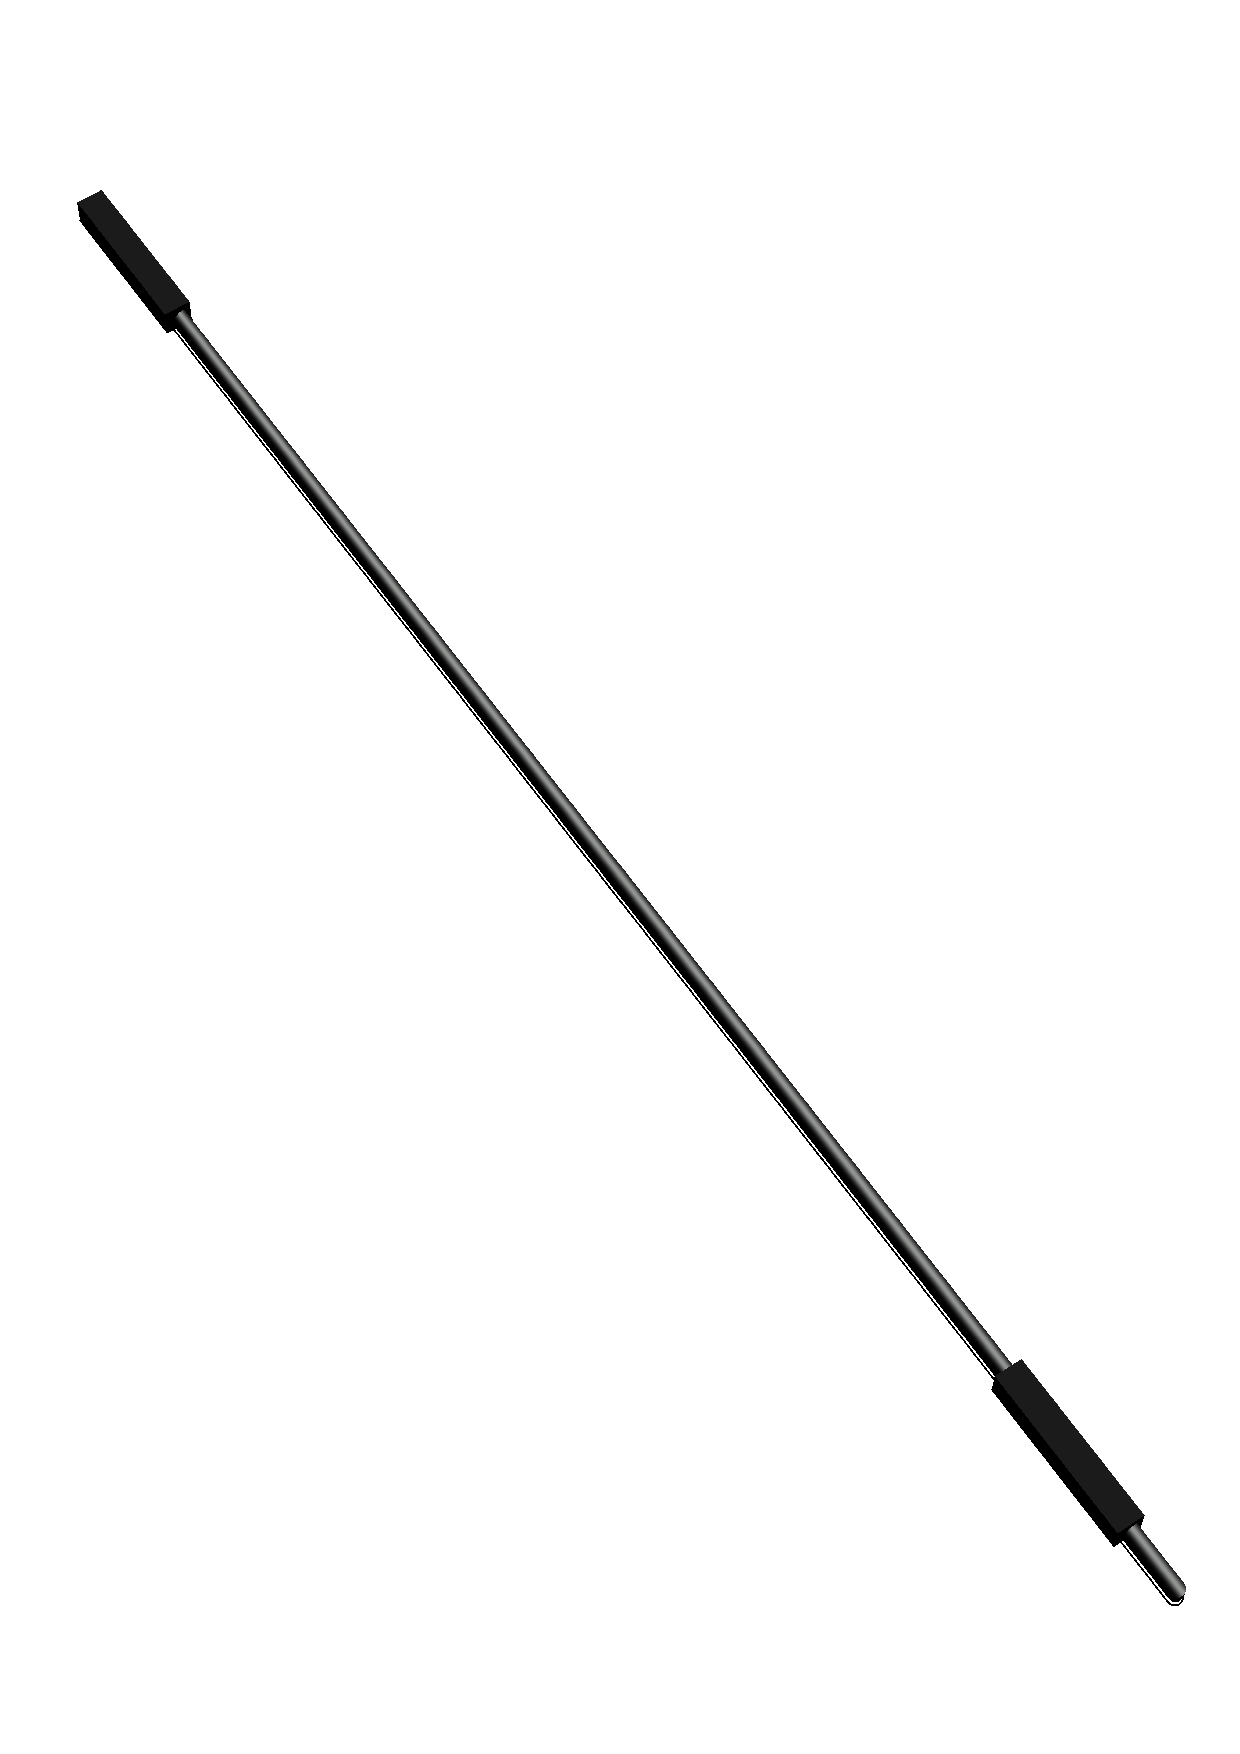
\includegraphics[scale=0.4]{15/img/cableJumperMHModelo.pdf}
        \caption{Cable Jumper Dupont Macho-Hembra 10cm en 3D.}
        \label{fig:cableJumperMHModelo}
    \end{figure}
    
    \subsubsection{Cable Jumper Dupont Macho-Macho 10cm}
    
    
    
    \begin{figure}[H]
        \centering
        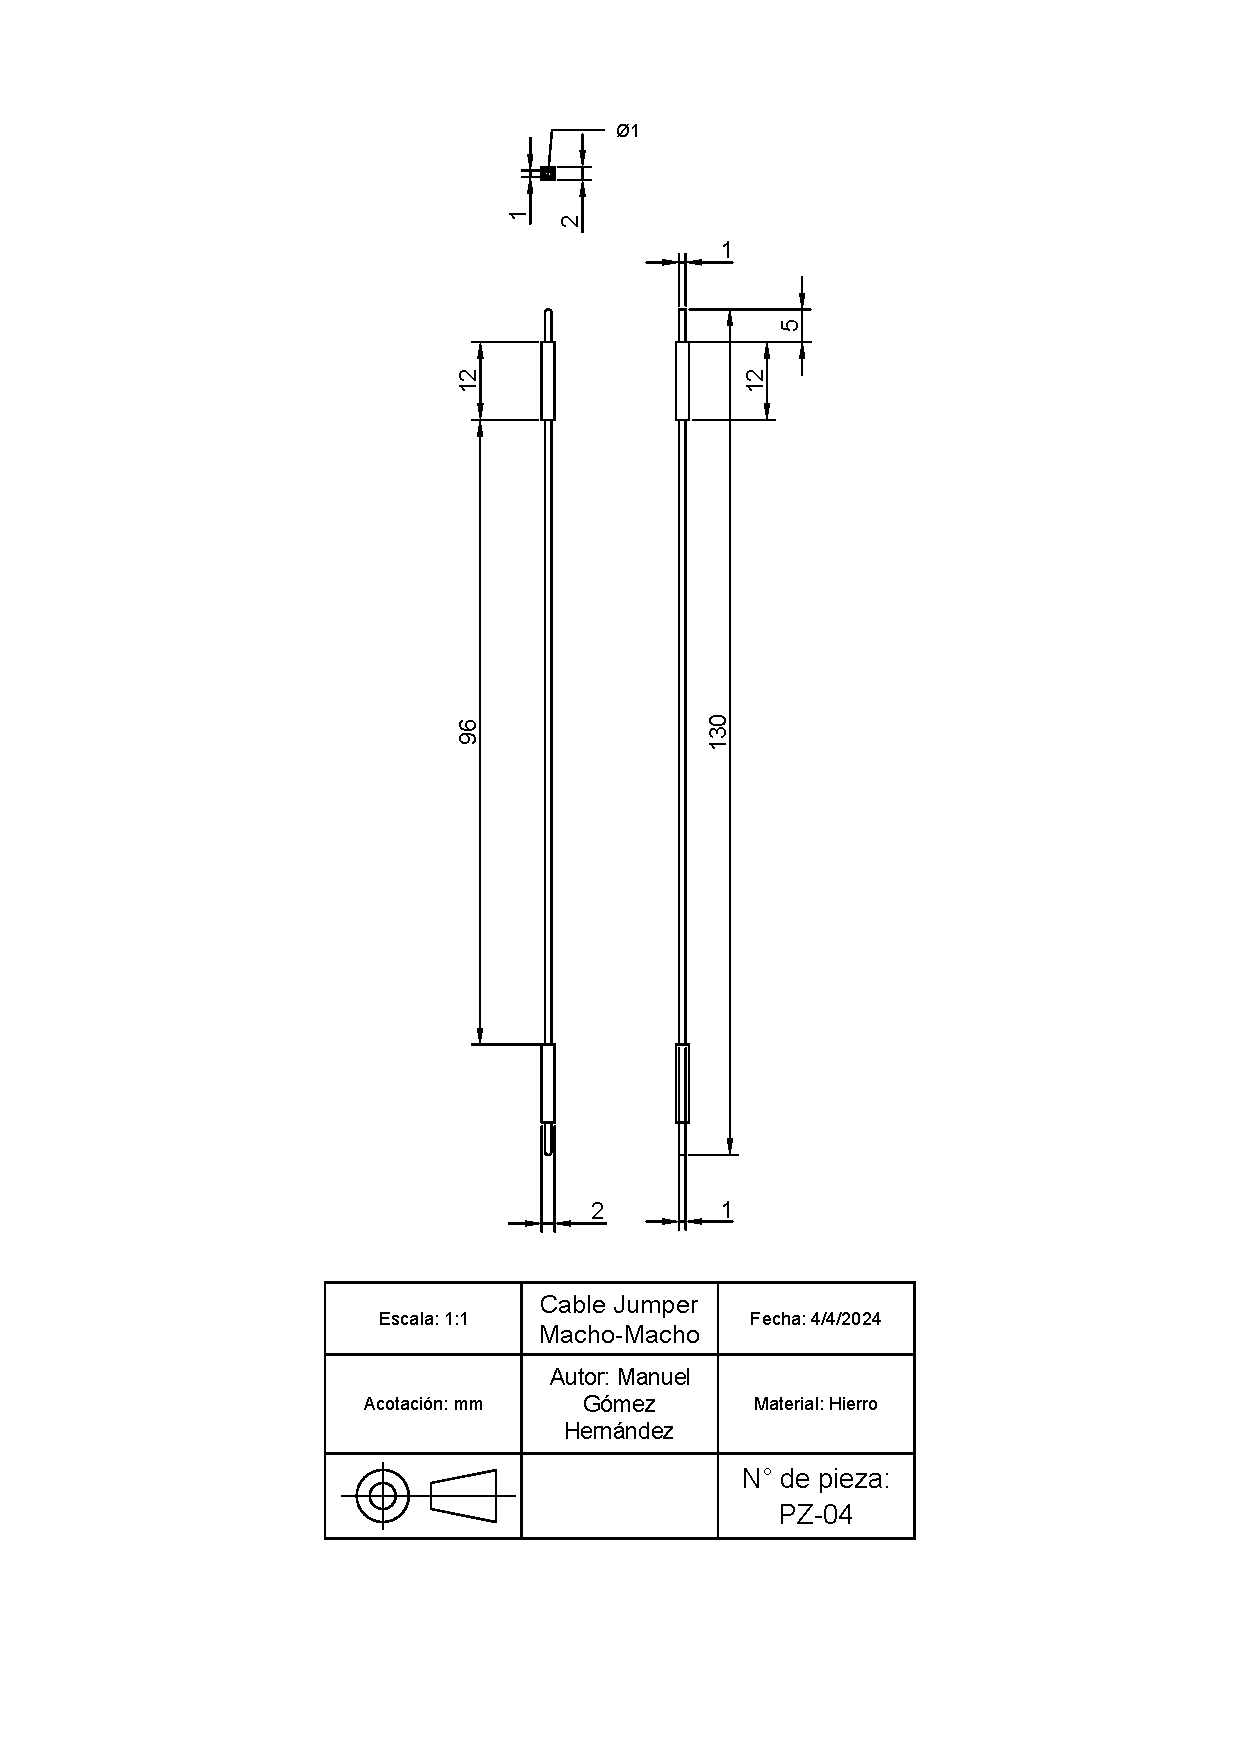
\includegraphics[scale=0.4]{15/img/cableJumperMMTrazo.pdf}
        \caption{Cable Jumper Dupont Macho-Macho 10cm con cotas.}
        \label{fig:cableJumperMMTrazo}
    \end{figure}
    
    \begin{figure}[H]
        \centering
        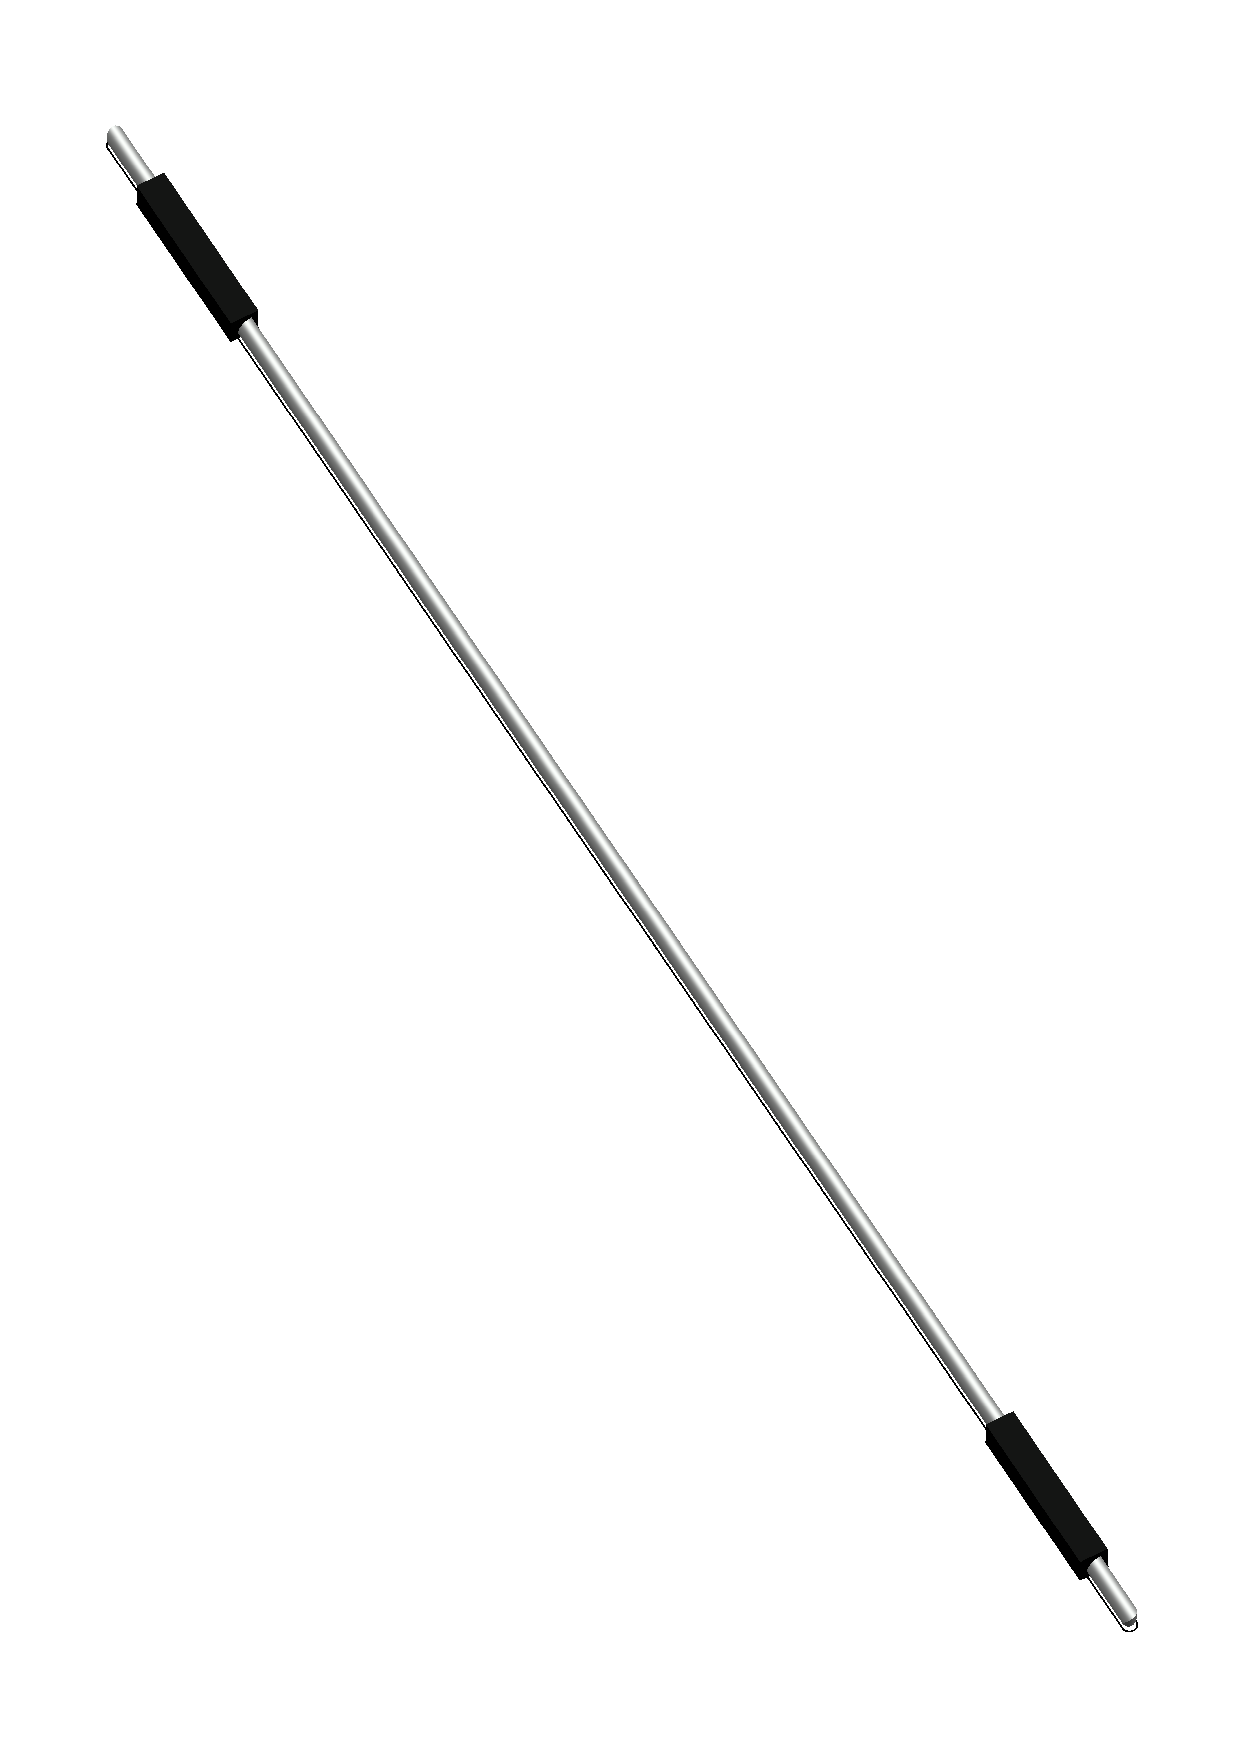
\includegraphics[scale=0.4]{15/img/cableJumperMMModelo.pdf}
        \caption{Cable Jumper Dupont Macho-Macho 10cm en 3D.}
        \label{fig:cableJumperMMModelo}
    \end{figure}
    
    \subsubsection{Potenciometro}
    
    
    
    \begin{figure}[H]
        \centering
        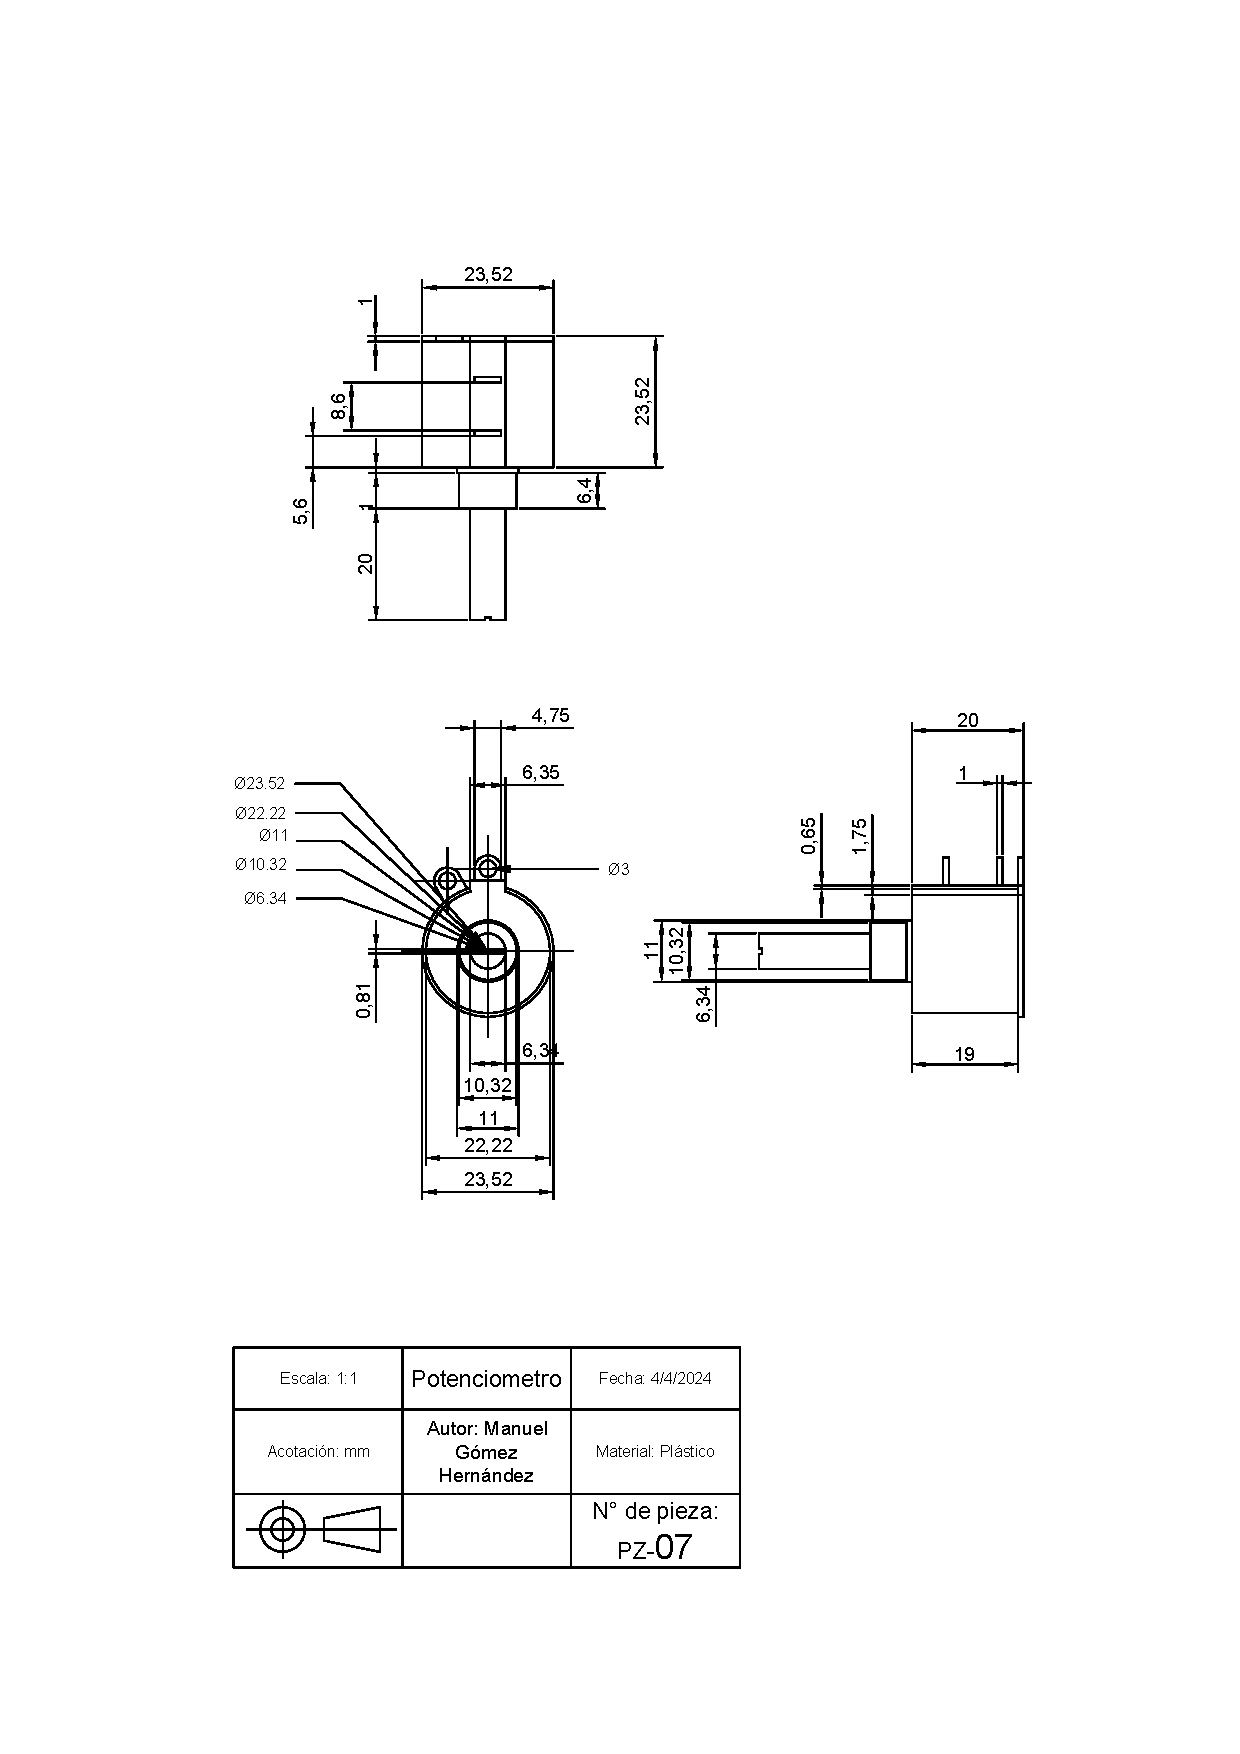
\includegraphics[scale=0.4]{15/img/potenciometroTrazo.pdf}
        \caption{Potencimetro con cotas.}
        \label{fig:potenciometroTrazo}
    \end{figure}
    
    \begin{figure}[H]
        \centering
        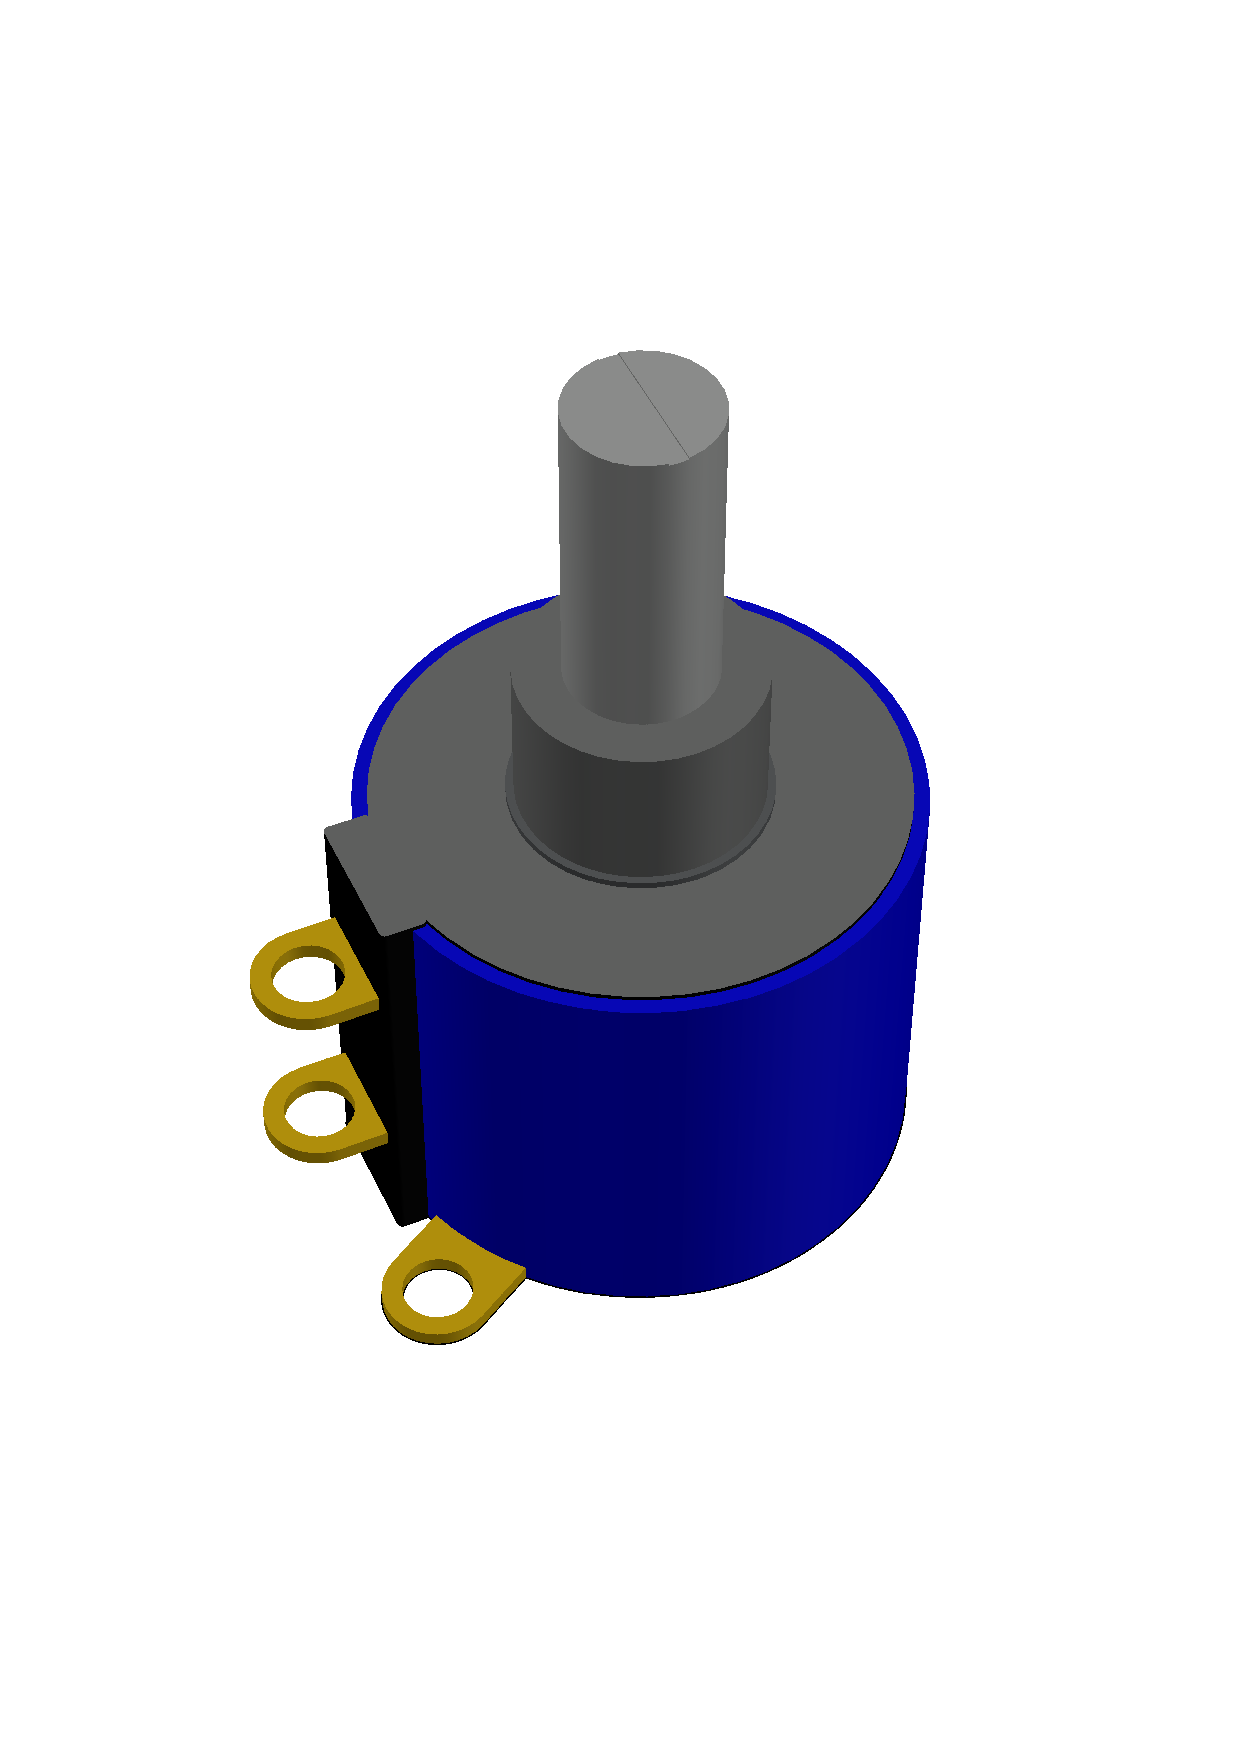
\includegraphics[scale=0.4]{15/img/potenciometroModelo.pdf}
        \caption{Potencimetro en 3D.}
        \label{fig:potenciometroModelo}
    \end{figure}
    
    \subsubsection{Tapete de aislamiento magnético 45*30 cm}
    
    
    
    
    %\begin{figure}[H]
     %   \centering
      %  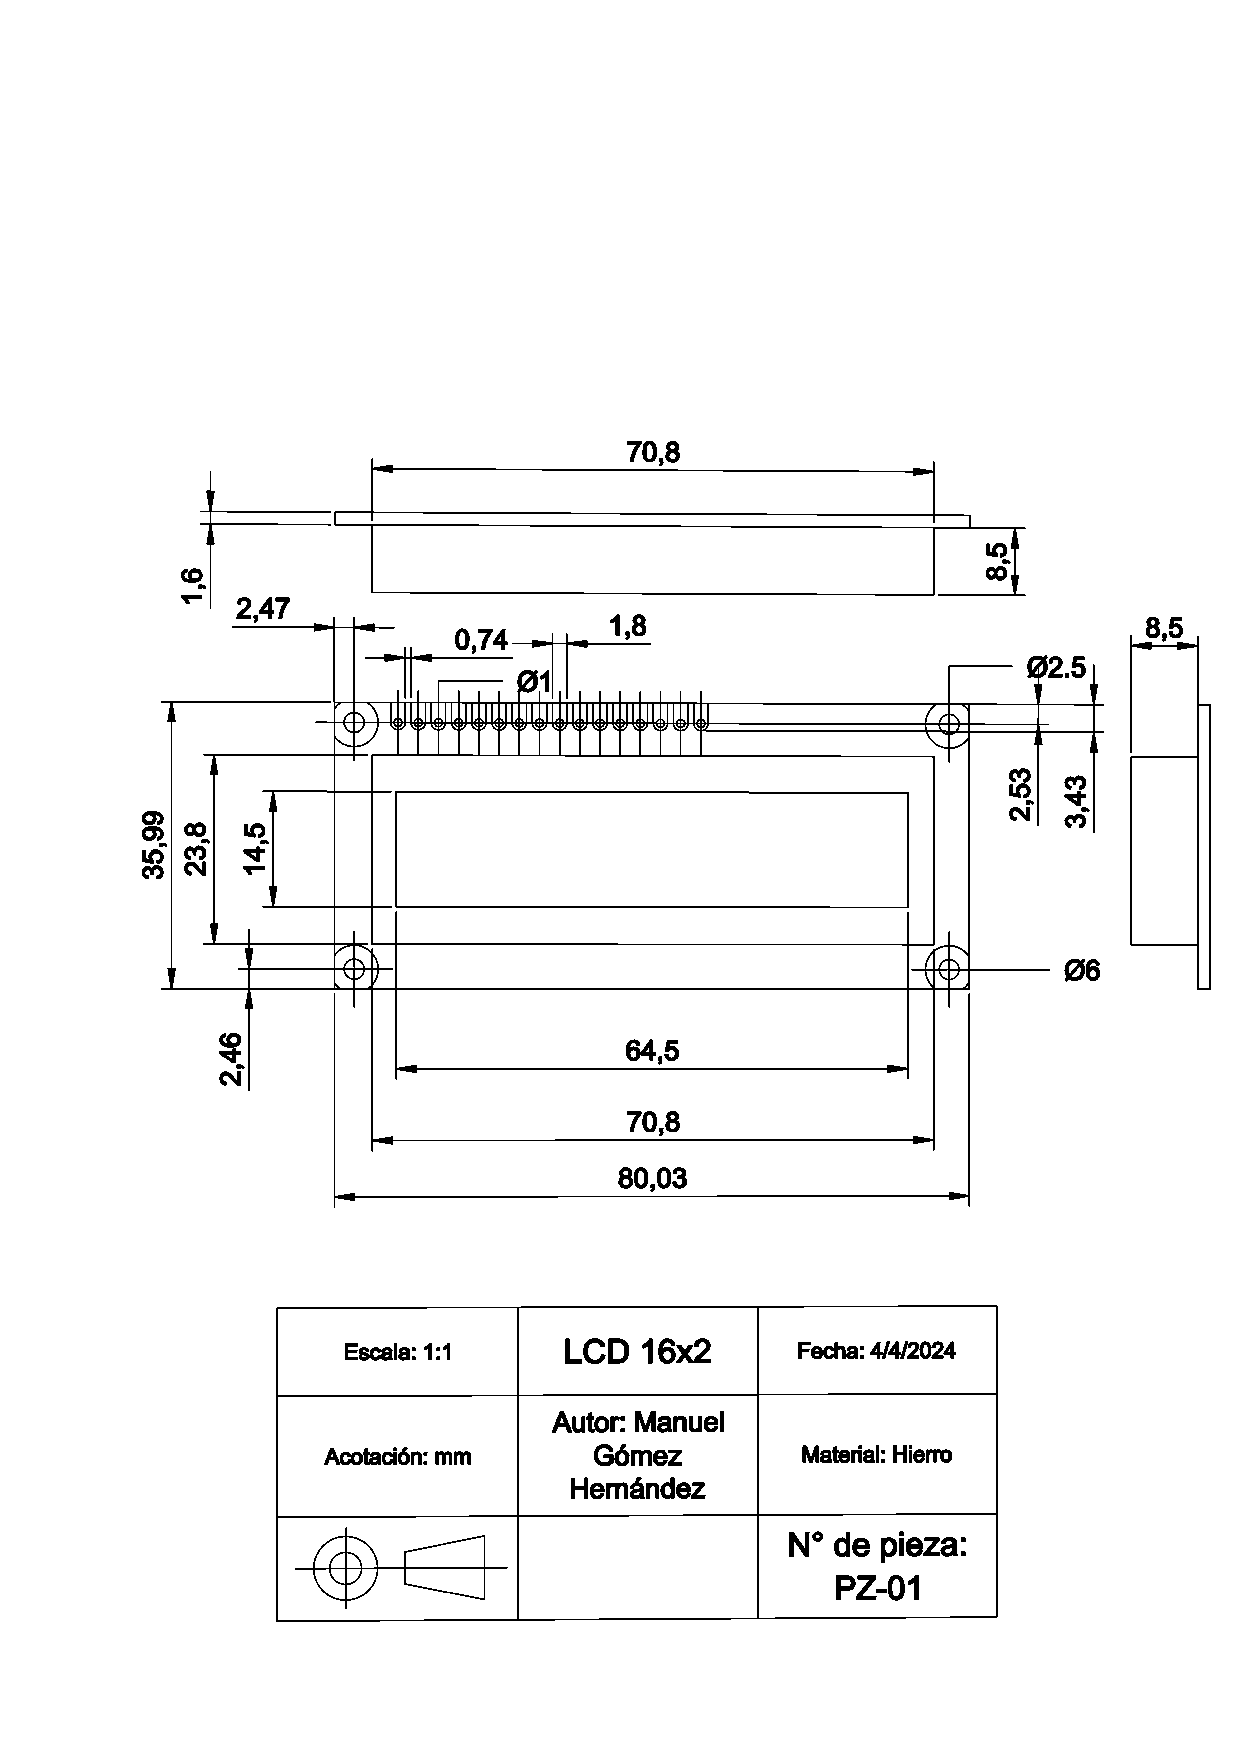
\includegraphics[scale=0.4]{15/img/lcdTrazo.pdf}
       % \caption{LCD 16x2.}
        %\label{fig:lcdTrazo}
    %\end{figure}
    % 
    \subsection{Determinación del tiempo estándar para que una persona competente realice el trabajo con marcha normal}
    

    El tiempo estándar para una operación dada es el tiempo requerido para que un operario de tipo medio, plenamente calificado y adiestrado, y trabajando a un ritmo normal, lleve a cabo la operación. Se determina sumando el tiempo asignado a todos los elementos comprendidos en el estudio de tiempos, tal y como se muestra en la siguiente tabla \ref{fig:tiempoEstandar}.
  
  
    Donde dicha tabla se ocupan las holguras o suplementos que se emplearon durante el ensamble, las cuales se dividen en dos partes: suplementos constantes y suplementos variables o por fatiga, los cuales se observan en la siguiente tabla \ref{fig:holguras} de igual forma se puede observar la separación entre hombre y mujer, para asi darnos el porcentaje para cada uno.
    
    Para determinar las holguras empleadas en el ensamble de dicho circuito, se necesita la siguiente tabla \ref{fig:tablaCalculoHolguras} donde se podra observar el apartado donde se coloca el porcentaje de cada una y al final se hace la suma de dichas holguras, las cuales ocuparan un espacio en la tabla para la determinación del tiempo estándar, 
  
  Teniendo cada uno de los elementos solicitados en la tabla de tiempo estándar \ref{fig:tiempoEstandar} y sustituirlos en la misma al igual que siguiendo cada una de las operaciones indicadas, se podrá obtener el tiempo estándar que se busca. 
    
  \begin{figure}[H]
      \centering
      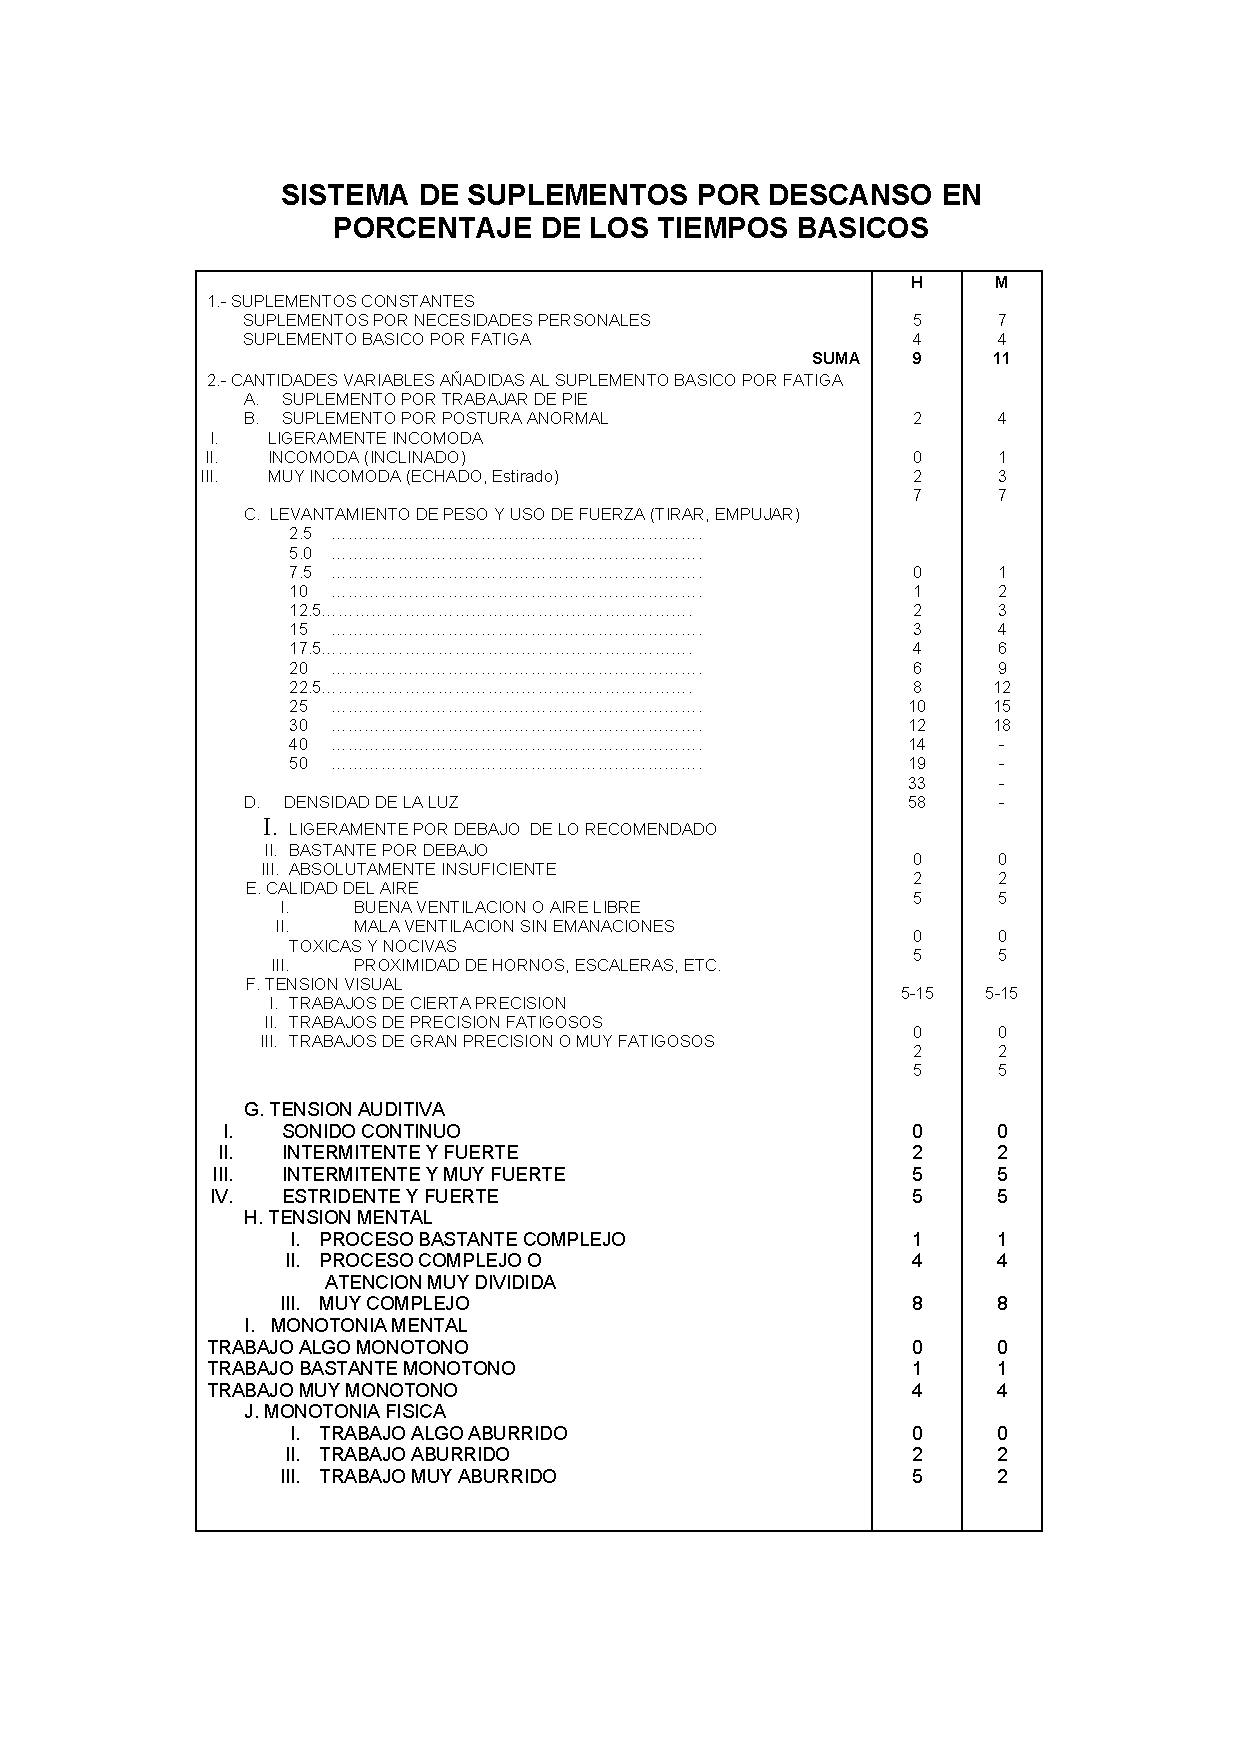
\includegraphics[scale=0.4]{15/img/tablaHolguras.pdf}
      \caption{Valores Asignado para Las Holguras o Suplementos.}
      \label{fig:holguras}
  \end{figure}
  
   \begin{figure}[H]
      \centering
      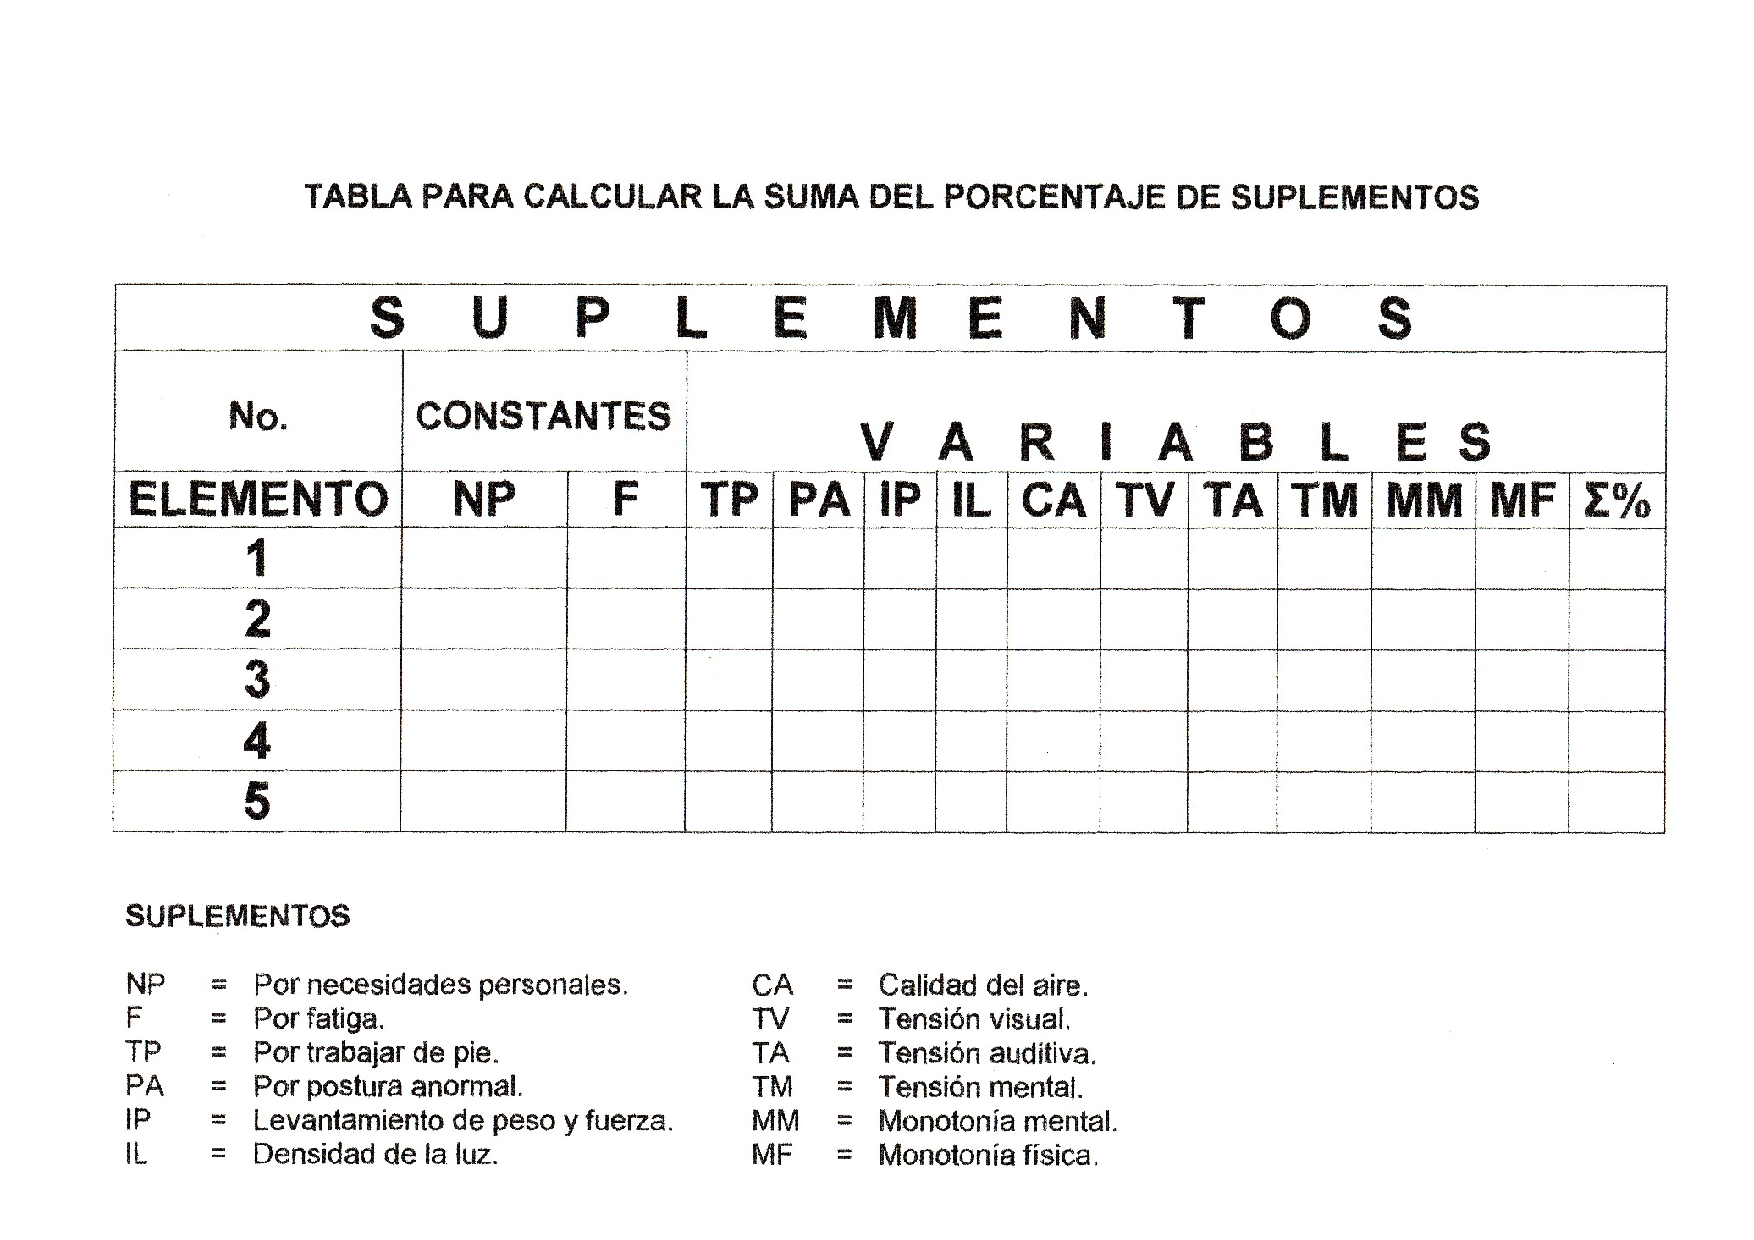
\includegraphics[scale=0.3]{15/img/tablaCalculoHolguras.pdf}
      \caption{Formato para el Calculo de Holguras.}
      \label{fig:tablaCalculoHolguras}
  \end{figure}
  
    \begin{figure}[H]
      \centering
      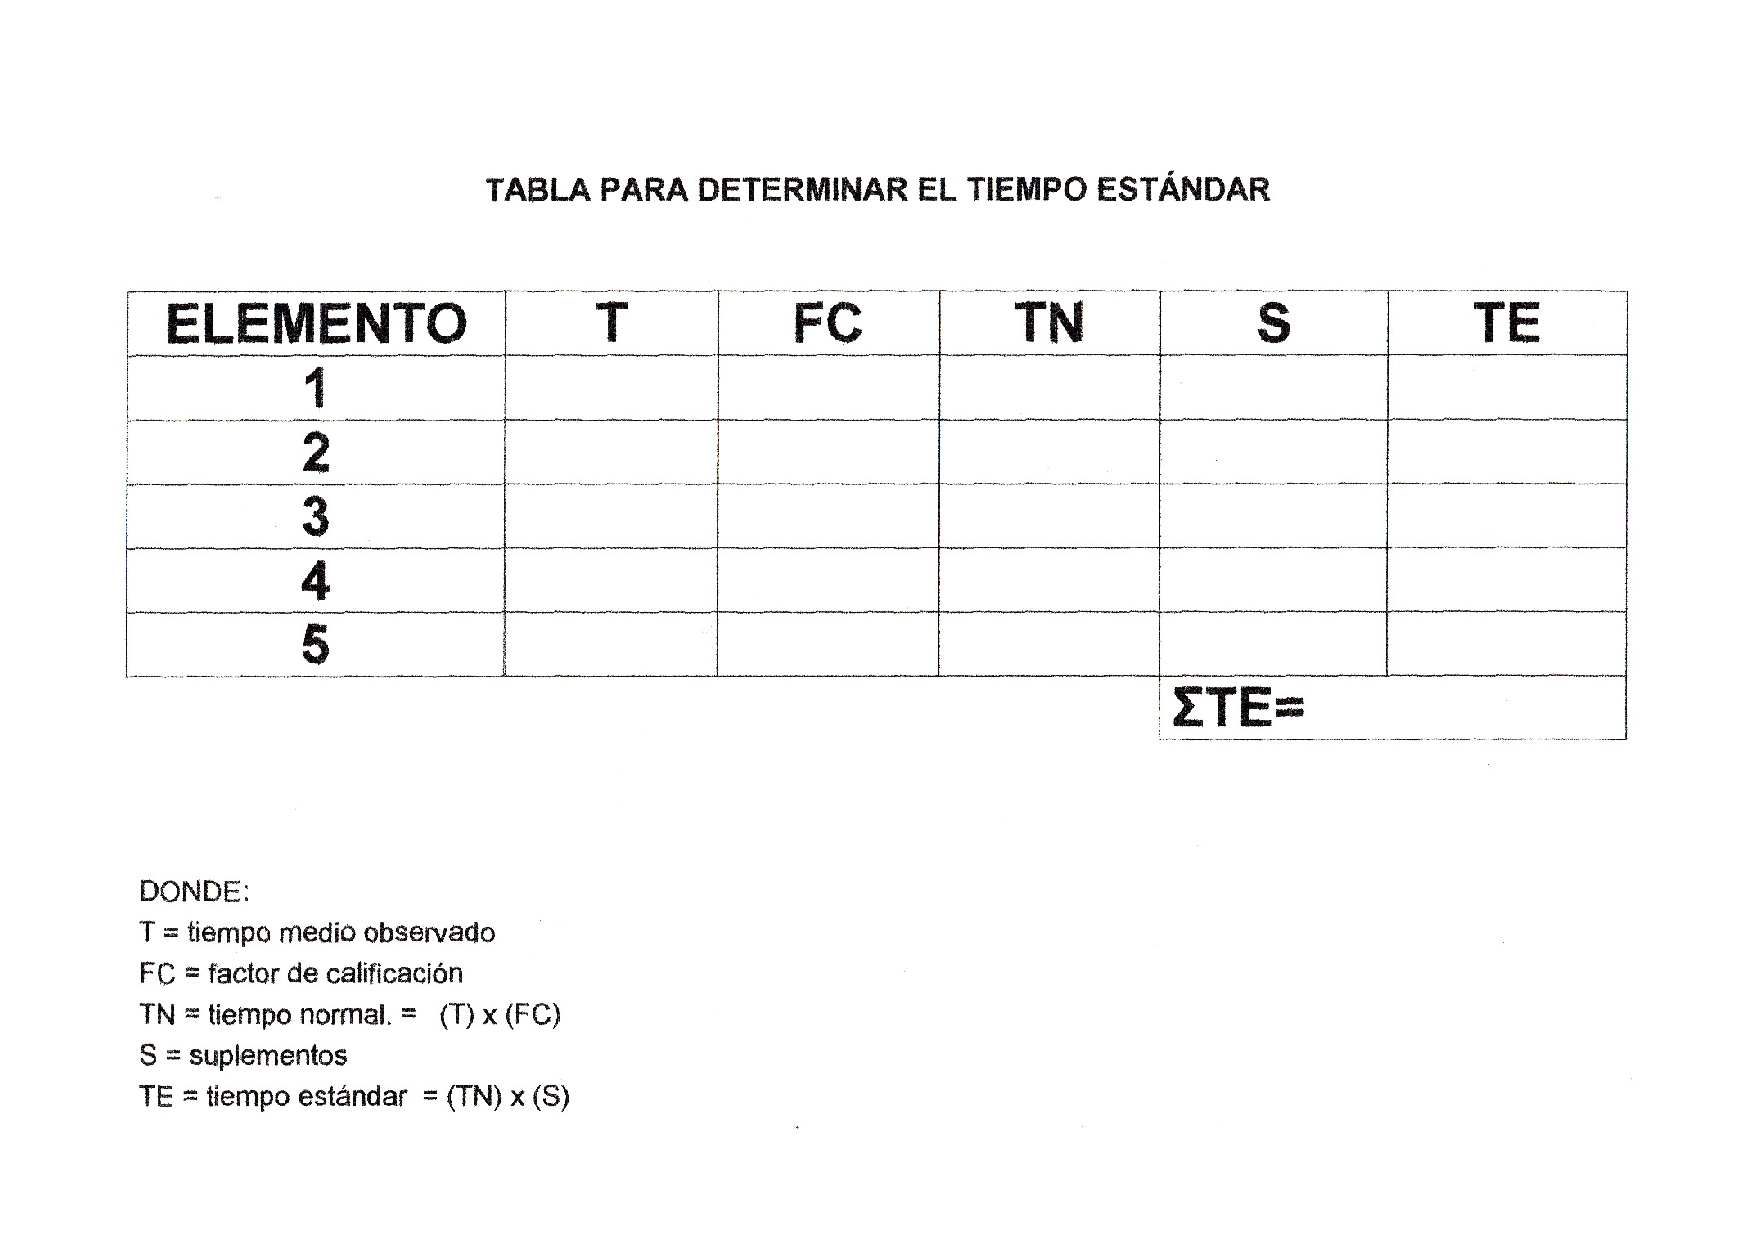
\includegraphics[scale=0.3]{15/img/tablaTiempoEstandar.pdf}
      \caption{Determinación de tiempo estándar.}
      \label{fig:tiempoEstandar}
  \end{figure}
   
     
    % 
    % 
    % Cada estrategia metodológica se establece acorde a cada objetivo, y por tanto deberá ser desglosada precisada y ordenada claramente. En consecuencia cada objetivo que se presentó en forma de verbo en infinitivo deberá determinar una estrategia en forma de adverbio. Ej. Desarrollar…Desarrollo. Son las actividades ordenadas que tienen como finalidad la prueba de la hipótesis. 
    
    % \begin{itemize}
    %     \item Se debe establecer que se habrá de hacer, como, conque, y donde para obtener la información que permita probar la hipótesis.  
    %     \item Se debe desglosar de acuerdo a los objetivos específicos. 
    %     \item Se debe establecer una estrategia metodológica por cada objetivo específico. De manera simplista se podría decir que se cambia el verbo en infinitivo por su respectivo adverbio.
    %     \item En cada objetivo se debe describir que método, que materiales y que equipo se usará para conseguirlo.
    %     \item Se deben tener referencias Figura \ref{fig:lcd-16x2}.
    % \end{itemize}
    % 
    % 
    % \begin{figure}[H]
    %     \centering
    %     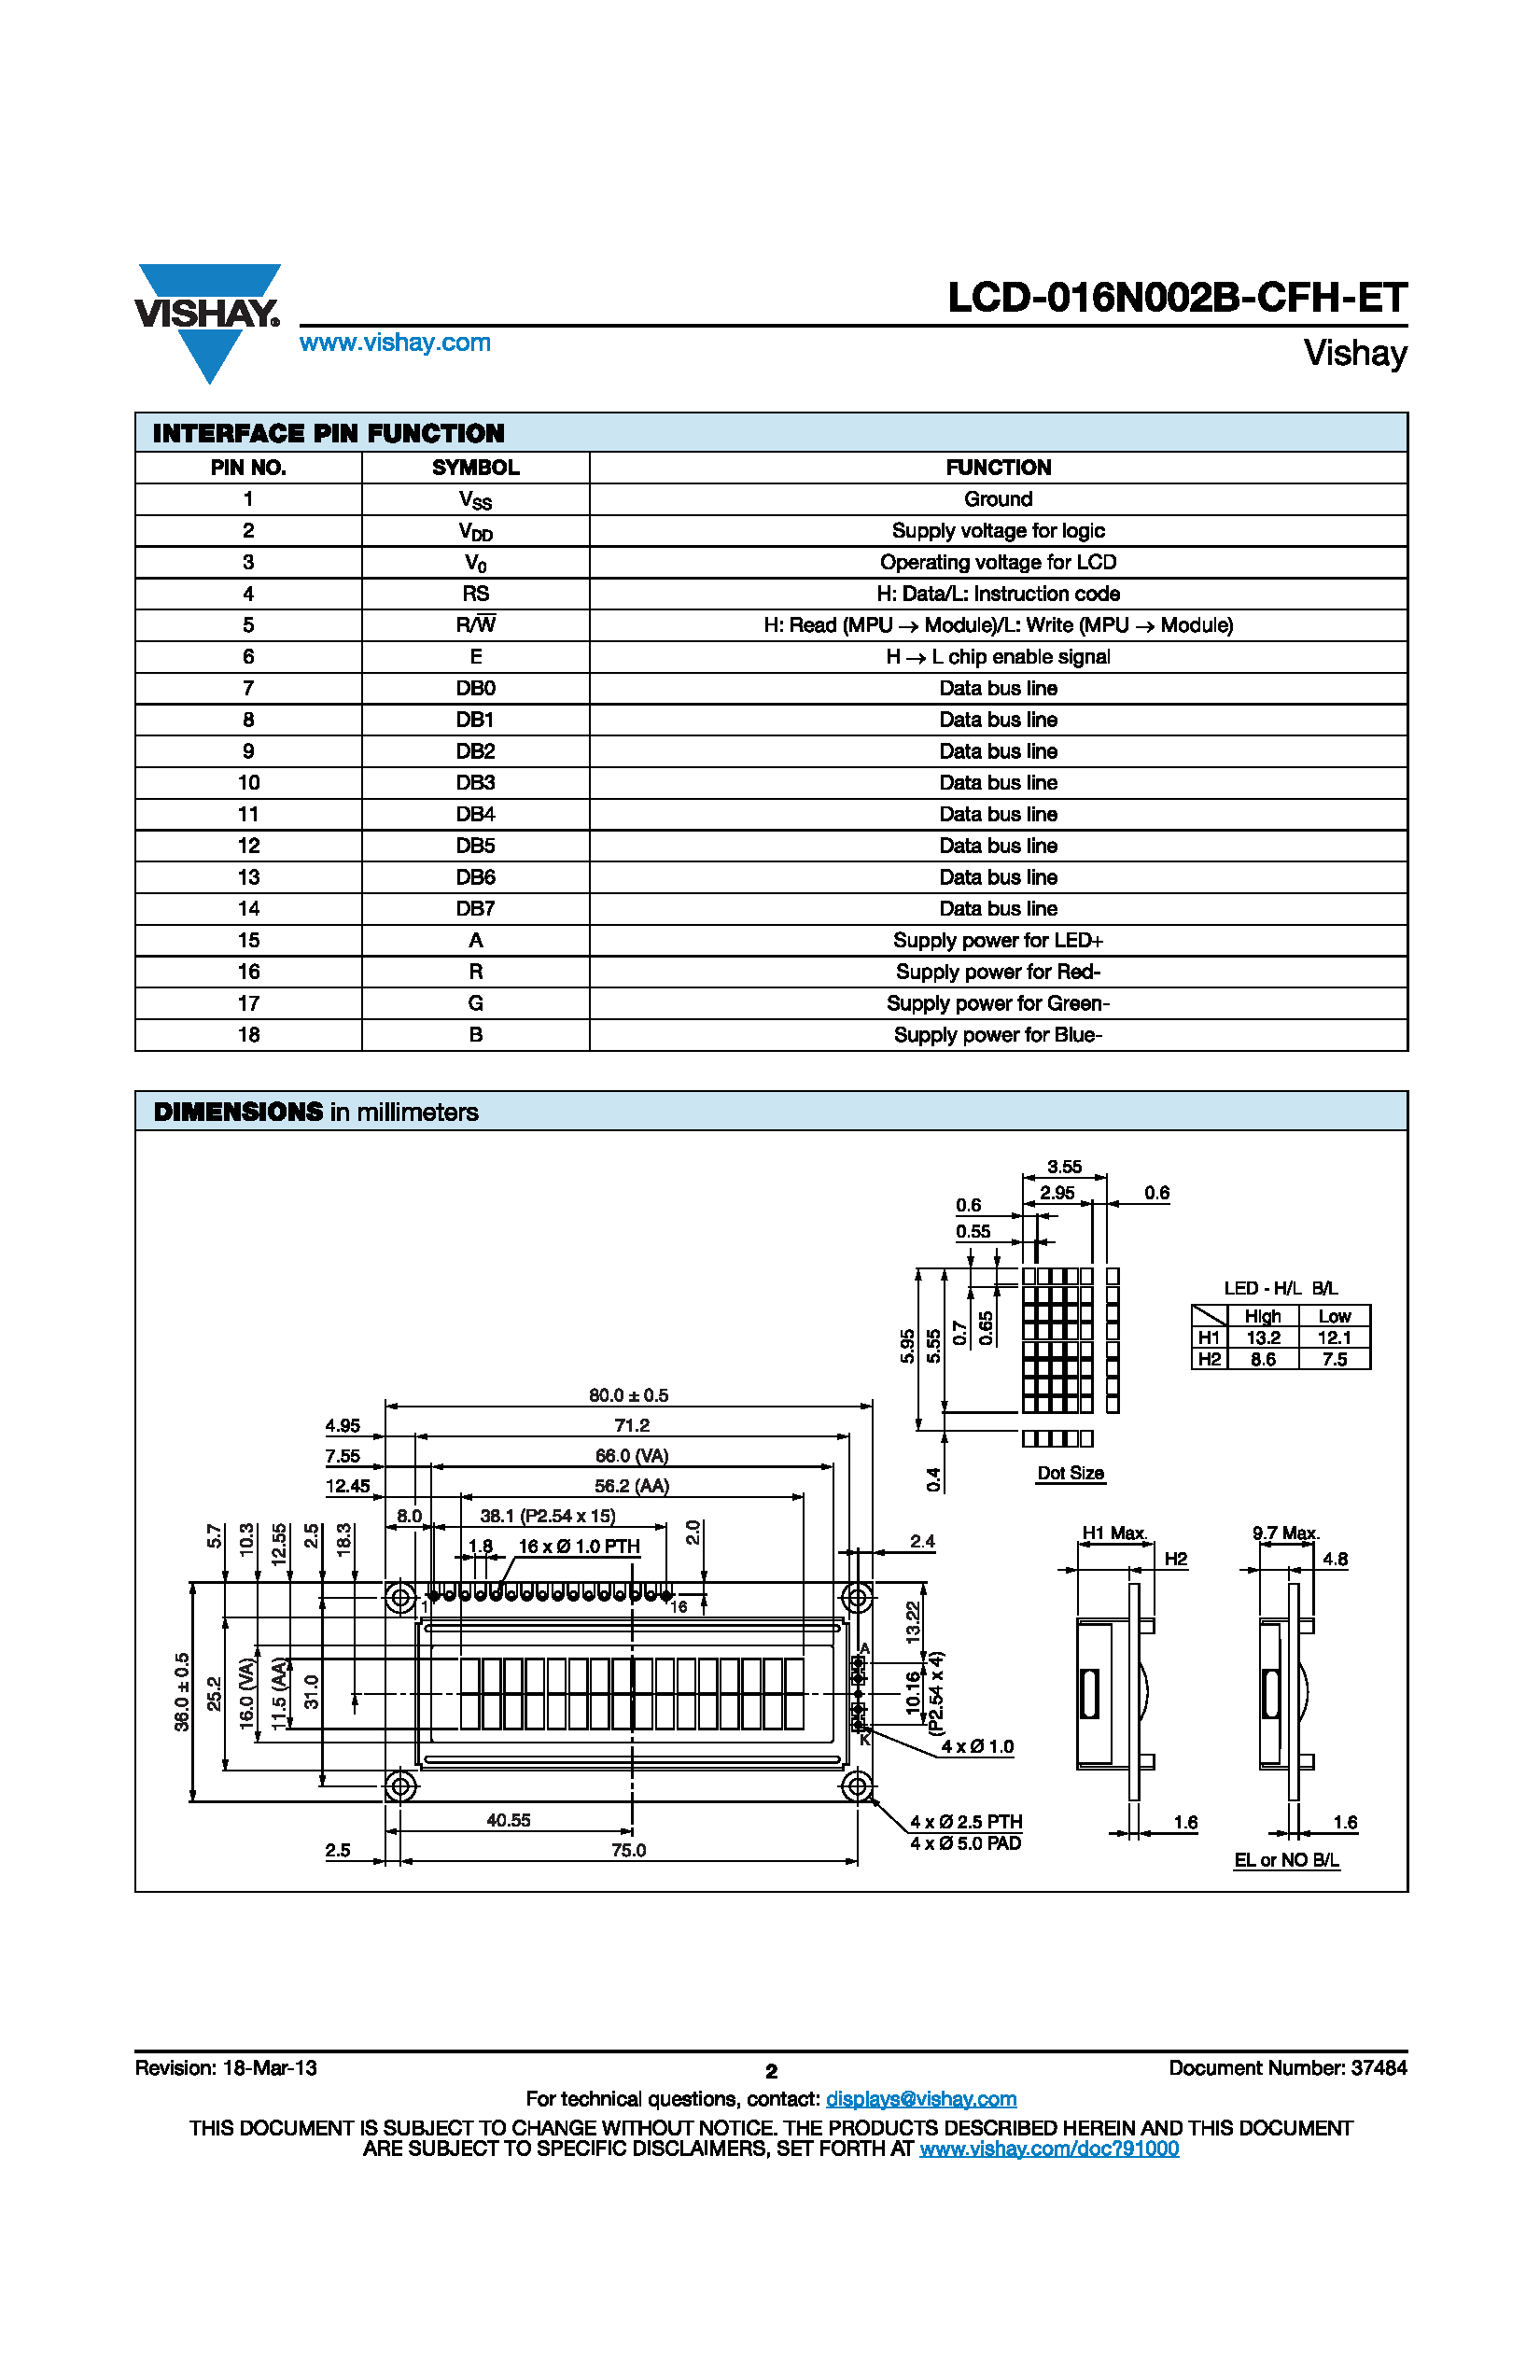
\includegraphics[trim = {30mm 65mm 90mm 250mm},clip,scale=0.5]{6/Img/lcd-16x2.pdf}
    %     \caption{Esquema LCD de 16x2}
    %     \label{fig:lcd-16x2}
    % \end{figure}
    % 
    % 
    % \begin{figure}[H]
    %     \centering
    %     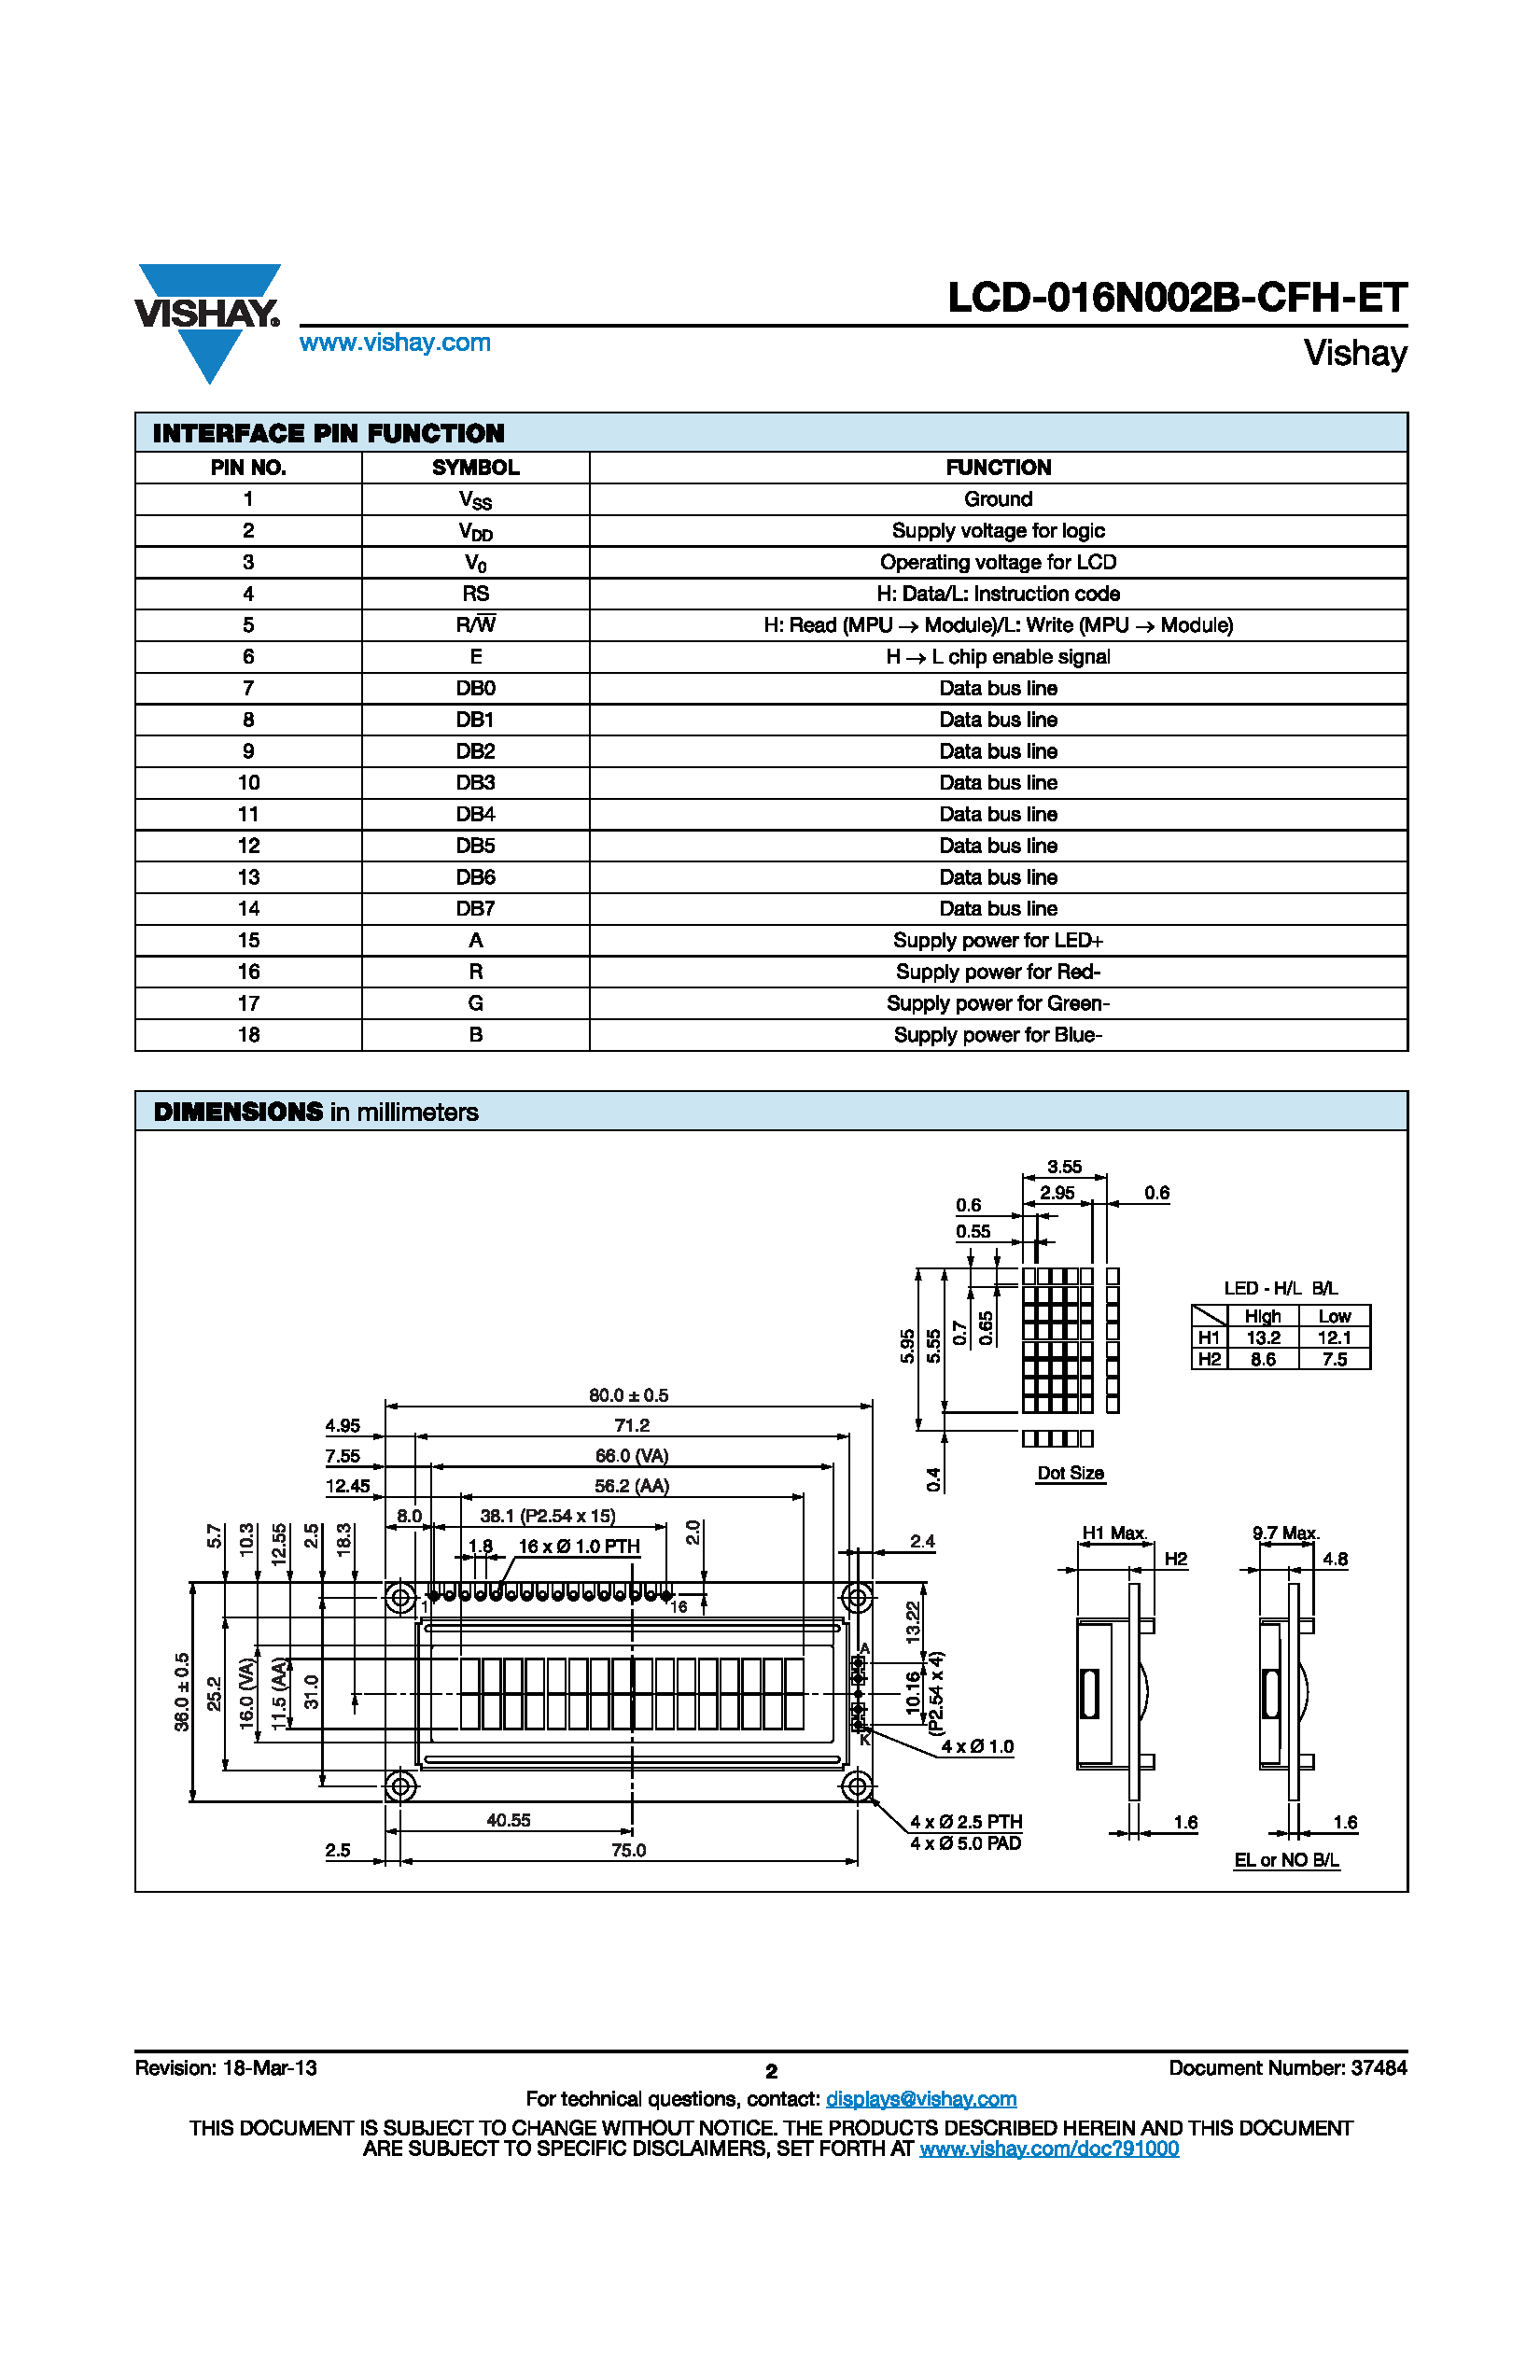
\includegraphics[trim = {30mm 250mm 90mm 20mm},clip,scale=0.5]{6/Img/lcd-16x2.pdf}
    %     \caption{Esquema LCD de 16x2}
    %     \label{fig:lcd}
    % \end{figure}
    % 
    % 
    % \subsection{Prepara tu documento}
    
    % Antes de que comiences a utilizar esta plantilla, es recomendable que prepare la información que contendrá en un archivo aparte. 
    % Ten preparadas tus gráficas, así como también las tablas aparte, para que sea más fácil integrarlo. 
    % Se recomienda fuertemente el uso de \textbf{formato Enhanced Metafile (.emf) para imágenes y gráficas} de resolución óptima. 
    % Finalmente, completa y organiza el contenido antes de darle el formato de esta plantilla. 
    
    \subsection{Acrónimos y Abreviaciones}
    
    Los acrónimos y abreviaciones deberán ser definidos únicamente la primera vez que aparecen en el texto, esto para que el lector entienda lo que significan.
    
    % \subsection{Ecuaciones}
    
    % Las ecuaciones son una excepción a las especificaciones prescritas de esta plantilla. 
    % Deberá determinar si su ecuación debe escribirse o no utilizando la fuente Adobe Devangari. 
    % Para crear ecuaciones multinivel, puede ser necesario tratar la ecuación como un gráfico e insertarla en el texto después de aplicar el estilo de la platilla.
    % Las ecuaciones serán enumeradas de manera consecutiva, y el número de ecuación, entre paréntesis, se colocan al ras de la derecha, utilizando una tabulación derecha.
    % 
    % \begin{equation}
    %     \label{eq1}
    %     x + y = z 
    % \end{equation}
    % 
    % Es importante asegurarse de que los símbolos de la ecuación sean definidos antes o inmediatamente después de la ecuación. Utilice “(1)”, en vez de “Eq. 1” al enumerar las ecuaciones, excepto al principio de una oración: “La ecuación (\ref{eq1}) es…”
    
    \section{Resultados y discusión}
    
    \subsection{Guía plan de Emergencia}
    
    Con esta guía, nuestro objetivo es reducir al mínimo las posibles emergencias de incendio y los riesgos de accidentes en el Instituto Tecnológico de Querétaro. Esto se logrará a través de capacitaciones anuales para el personal, que les permitirá tomar decisiones efectivas en situaciones de emergencia para proteger la seguridad de todas las personas dentro y fuera de la institución, así como la integridad de las instalaciones. Las especificaciónes de la Institución se resumen en la figura \ref{fig:mapaUbicacion}.
    
    \begin{figure}[H]
        \centering
        \includegraphics[scale=0.15]{15/img/mapaUbicacion.pdf}
        \caption{Instituto Tecnologico de Queretaro, Av. Tecnológivo s/n esq. Gral. Mariano Escobedo. Colonia Centro Histórico C.P. 76000, Querétaro, Querétaro, México. Tel. 442 227 4400, Correo: contacto@itq.edu.mx, Paguina Web: https://queretaro.tecnm.mx. 
        Cuenta con una	superficie total de 78,271.42 m2 o 842,506.55 Pies2 aproximadamente, asi como un total de 5,696 estudiantes aproximadamente tanto de pregrado como posgrado y una planta academica para programas de Licenciaturas de 236 docentes y para Estudios de posgrado 6 docentes, dando uun total de 242 docentes, Dicho instituto tiene como director al Ing. Ramón Soto Arriola. }
        \label{fig:mapaUbicacion}
    \end{figure}
    
    \subsubsection{Identificación del riesgo}
    
    Nos comprometemos a implementar diariamente un programa interno como externo de prevención de riesgos, además de solicitar retroalimentación tanto de clientes internos como externos sobre los riesgos presentes en nuestras actividades regulares. Invitando activamente al equipo de trabajo a participar en este proceso. 
    
    Cada riesgo interno y externo será evaluado y clasificado en función de su nivel de importancia, lo que nos permitirá priorizar nuestras acciones y tomar medidas adecuadas para abordarlos véase Figura \ref{fig:nivelesDeRiesgos}.
    
     \begin{figure}[H]
        \centering
        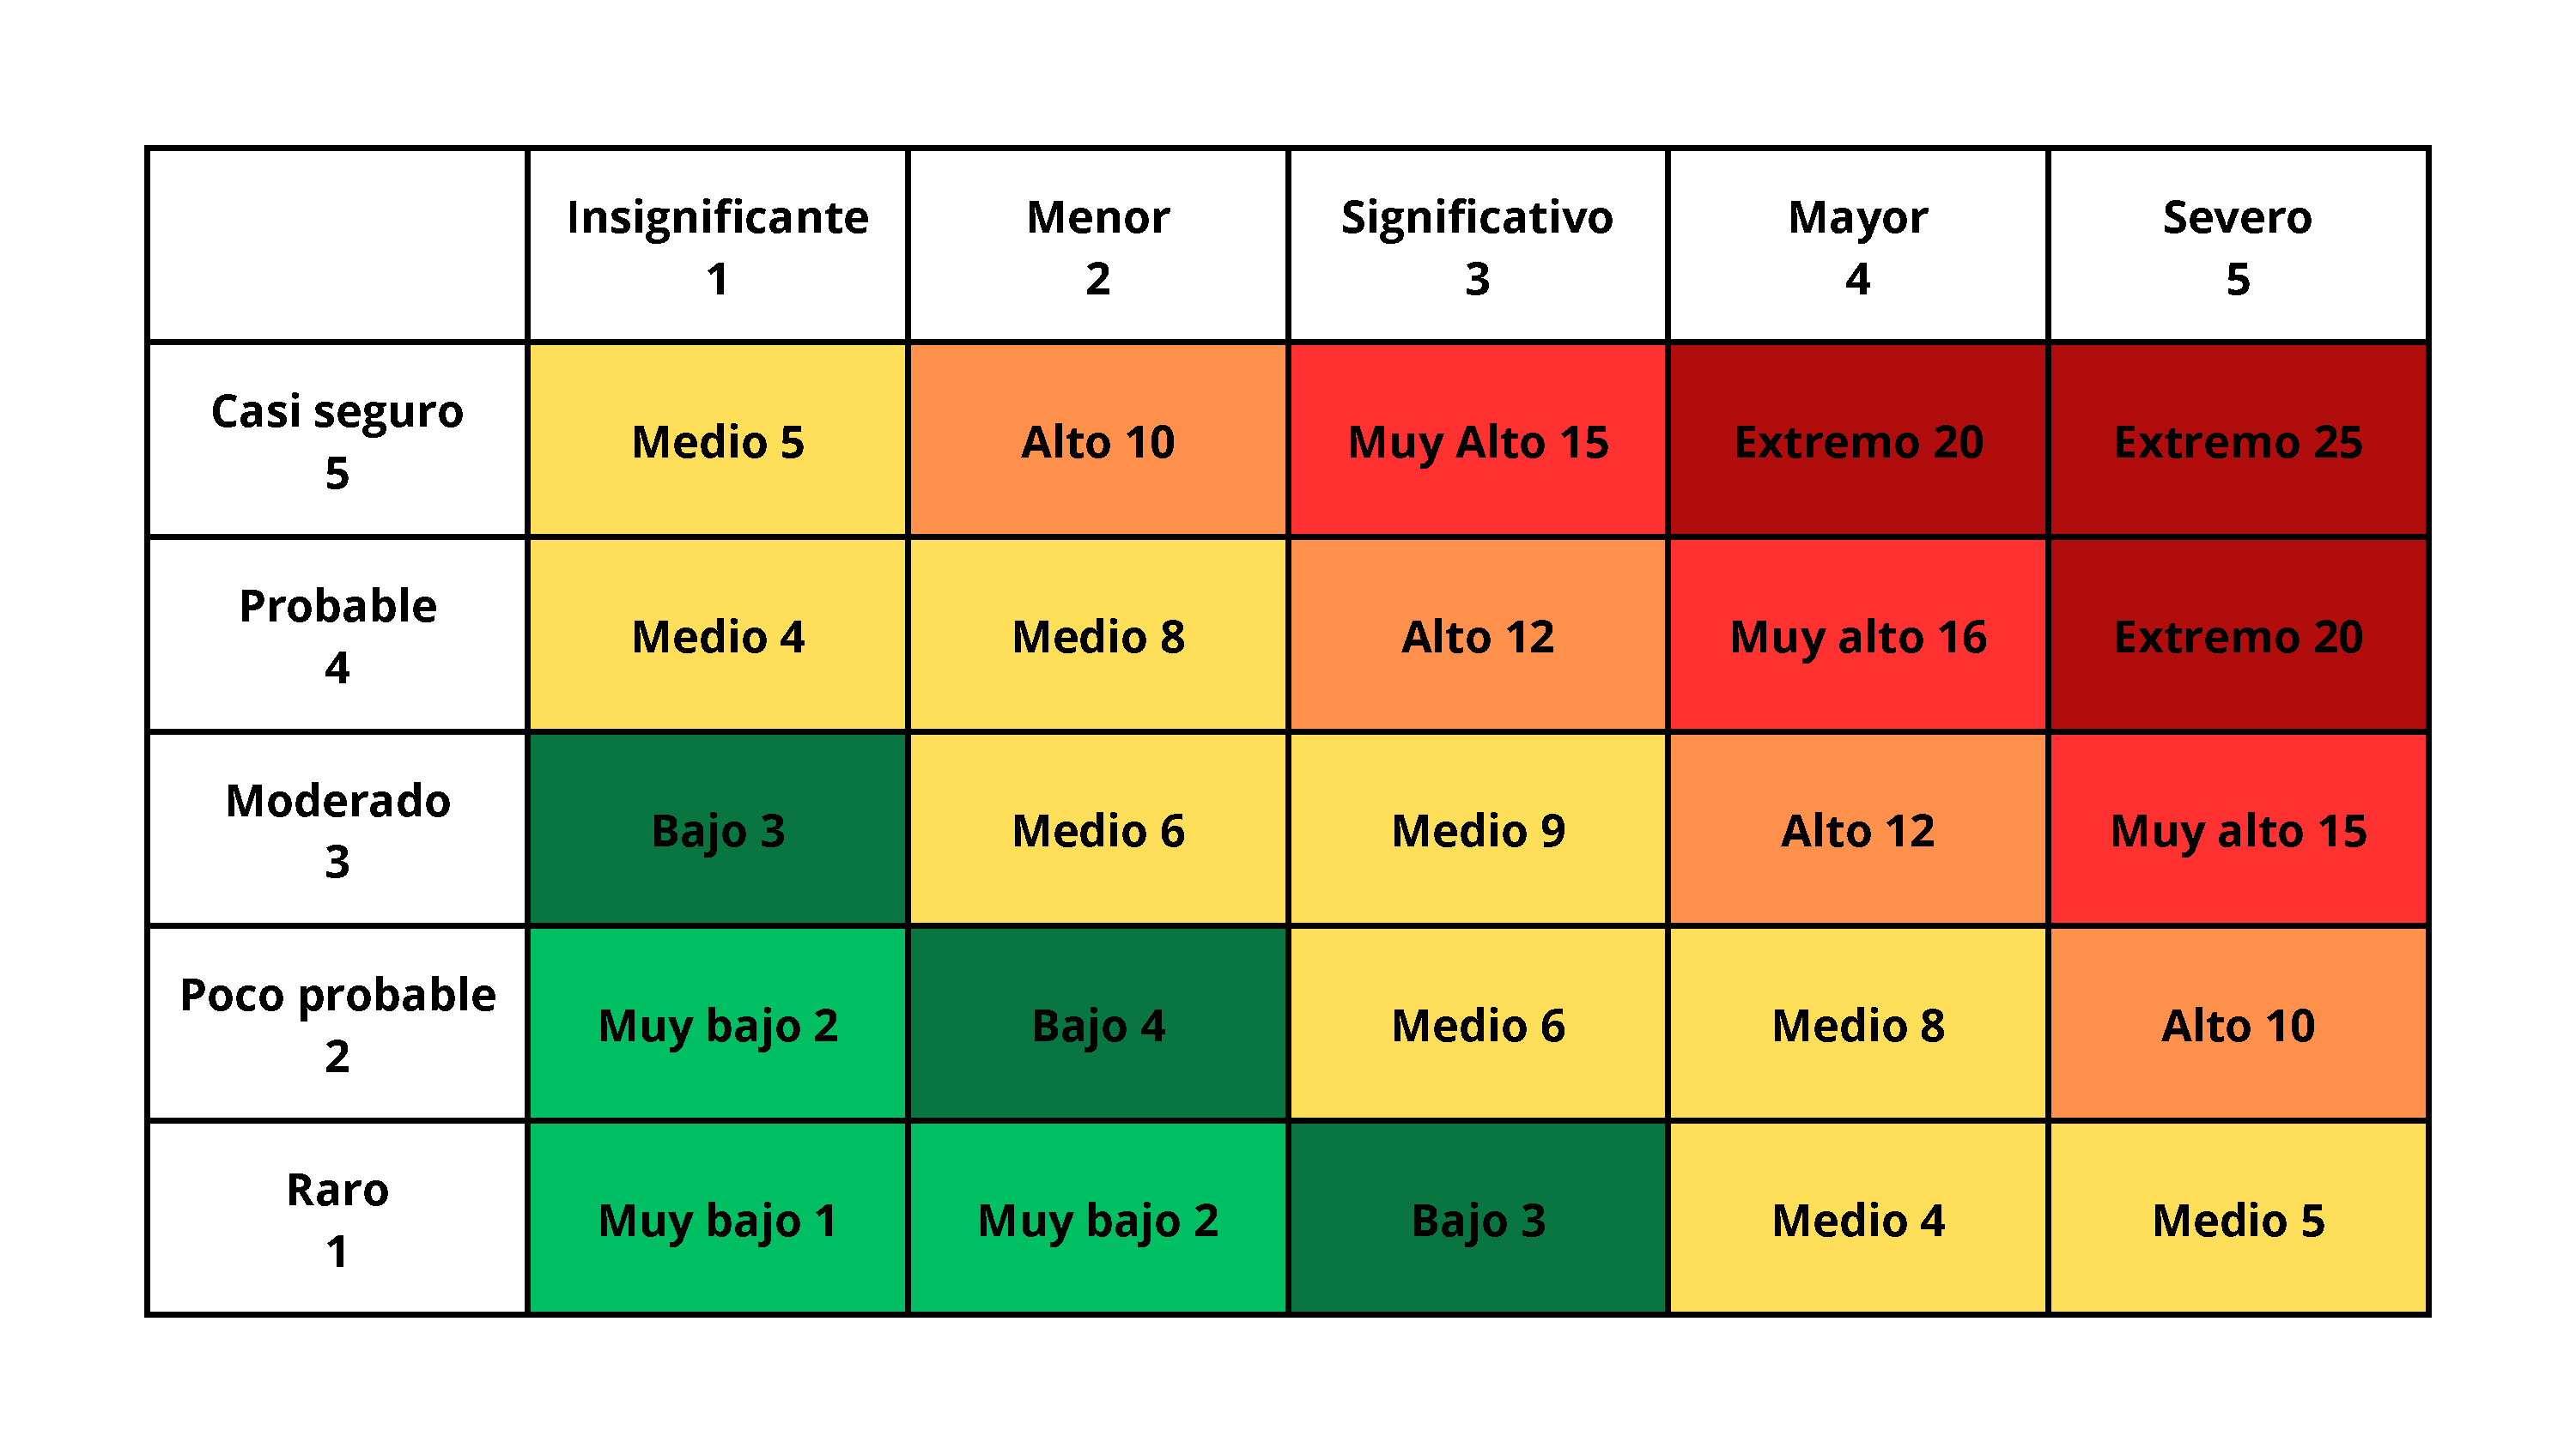
\includegraphics[scale=0.17]{15/img/nivelesDeRiesgos.pdf}
        \caption{Matriz de riesgos.}
        \label{fig:nivelesDeRiesgos}
    \end{figure}
    
    \subsubsection{Riesgos internos}
    
    El concepto de riesgo implica la probabilidad de que un evento ocurra o no, representando la cercanía de un posible daño. En términos más simples, se refiere a la probabilidad de que algo ocurra, vease la siguiente tabla los riesgos Identificados.
    
    Por otro lado, el riesgo operativo interno se define como la probabilidad de que la empresa experimente pérdidas debido a fallas o deficiencias en sus propios procesos o funciones naturales de operación. Específicamente, se refiere a los riesgos que surgen internamente dentro de la empresa como resultado de su propio funcionamiento, siguiendo el diagrama que muestra la Figura \ref{fig:diagramaIdentificacionRiesgosAcciones}, obteniendo como resultado la siguiente tabla \ref{fig:tablaRiesgosInternos}.
    
    \begin{figure}[H]
        \centering
        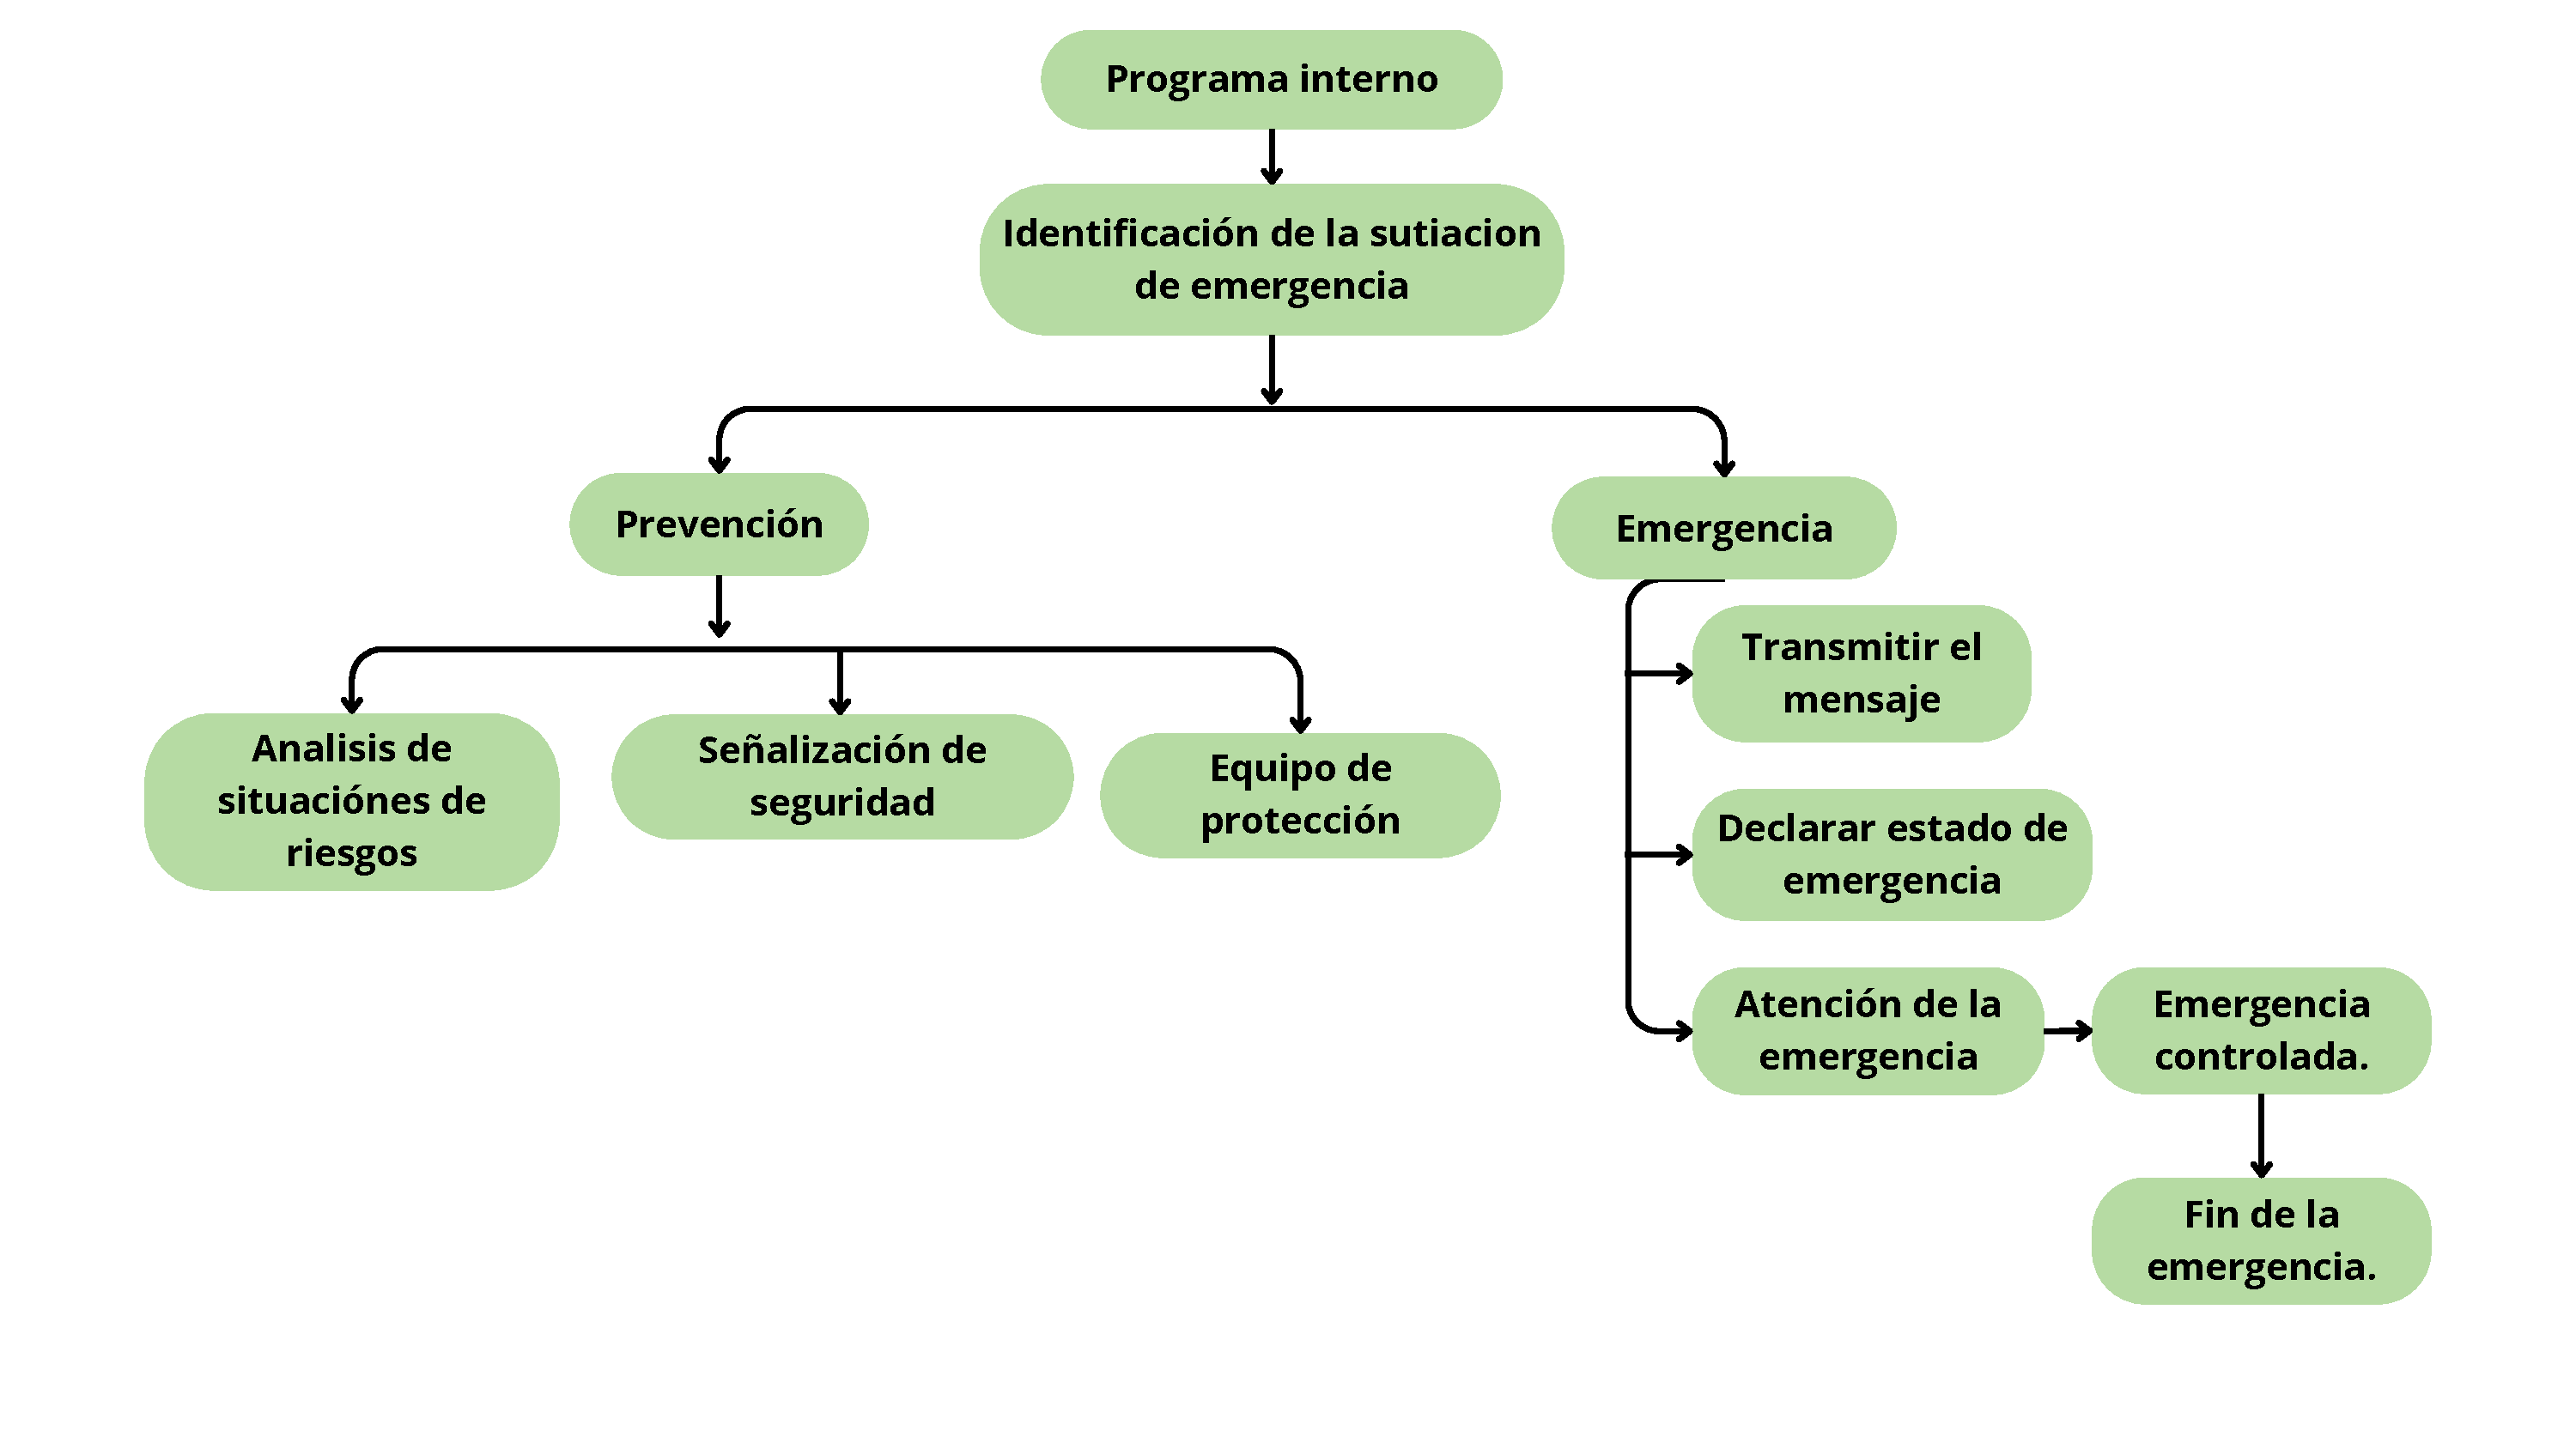
\includegraphics[scale=0.17]{15/img/diagramaIdentifiacionRiesgosAcciones.pdf}
        \caption{Diagrama para la identificación de riesgos y acciones.}
        \label{fig:diagramaIdentificacionRiesgosAcciones}
    \end{figure}
    
    \begin{figure}[H]
        \centering
        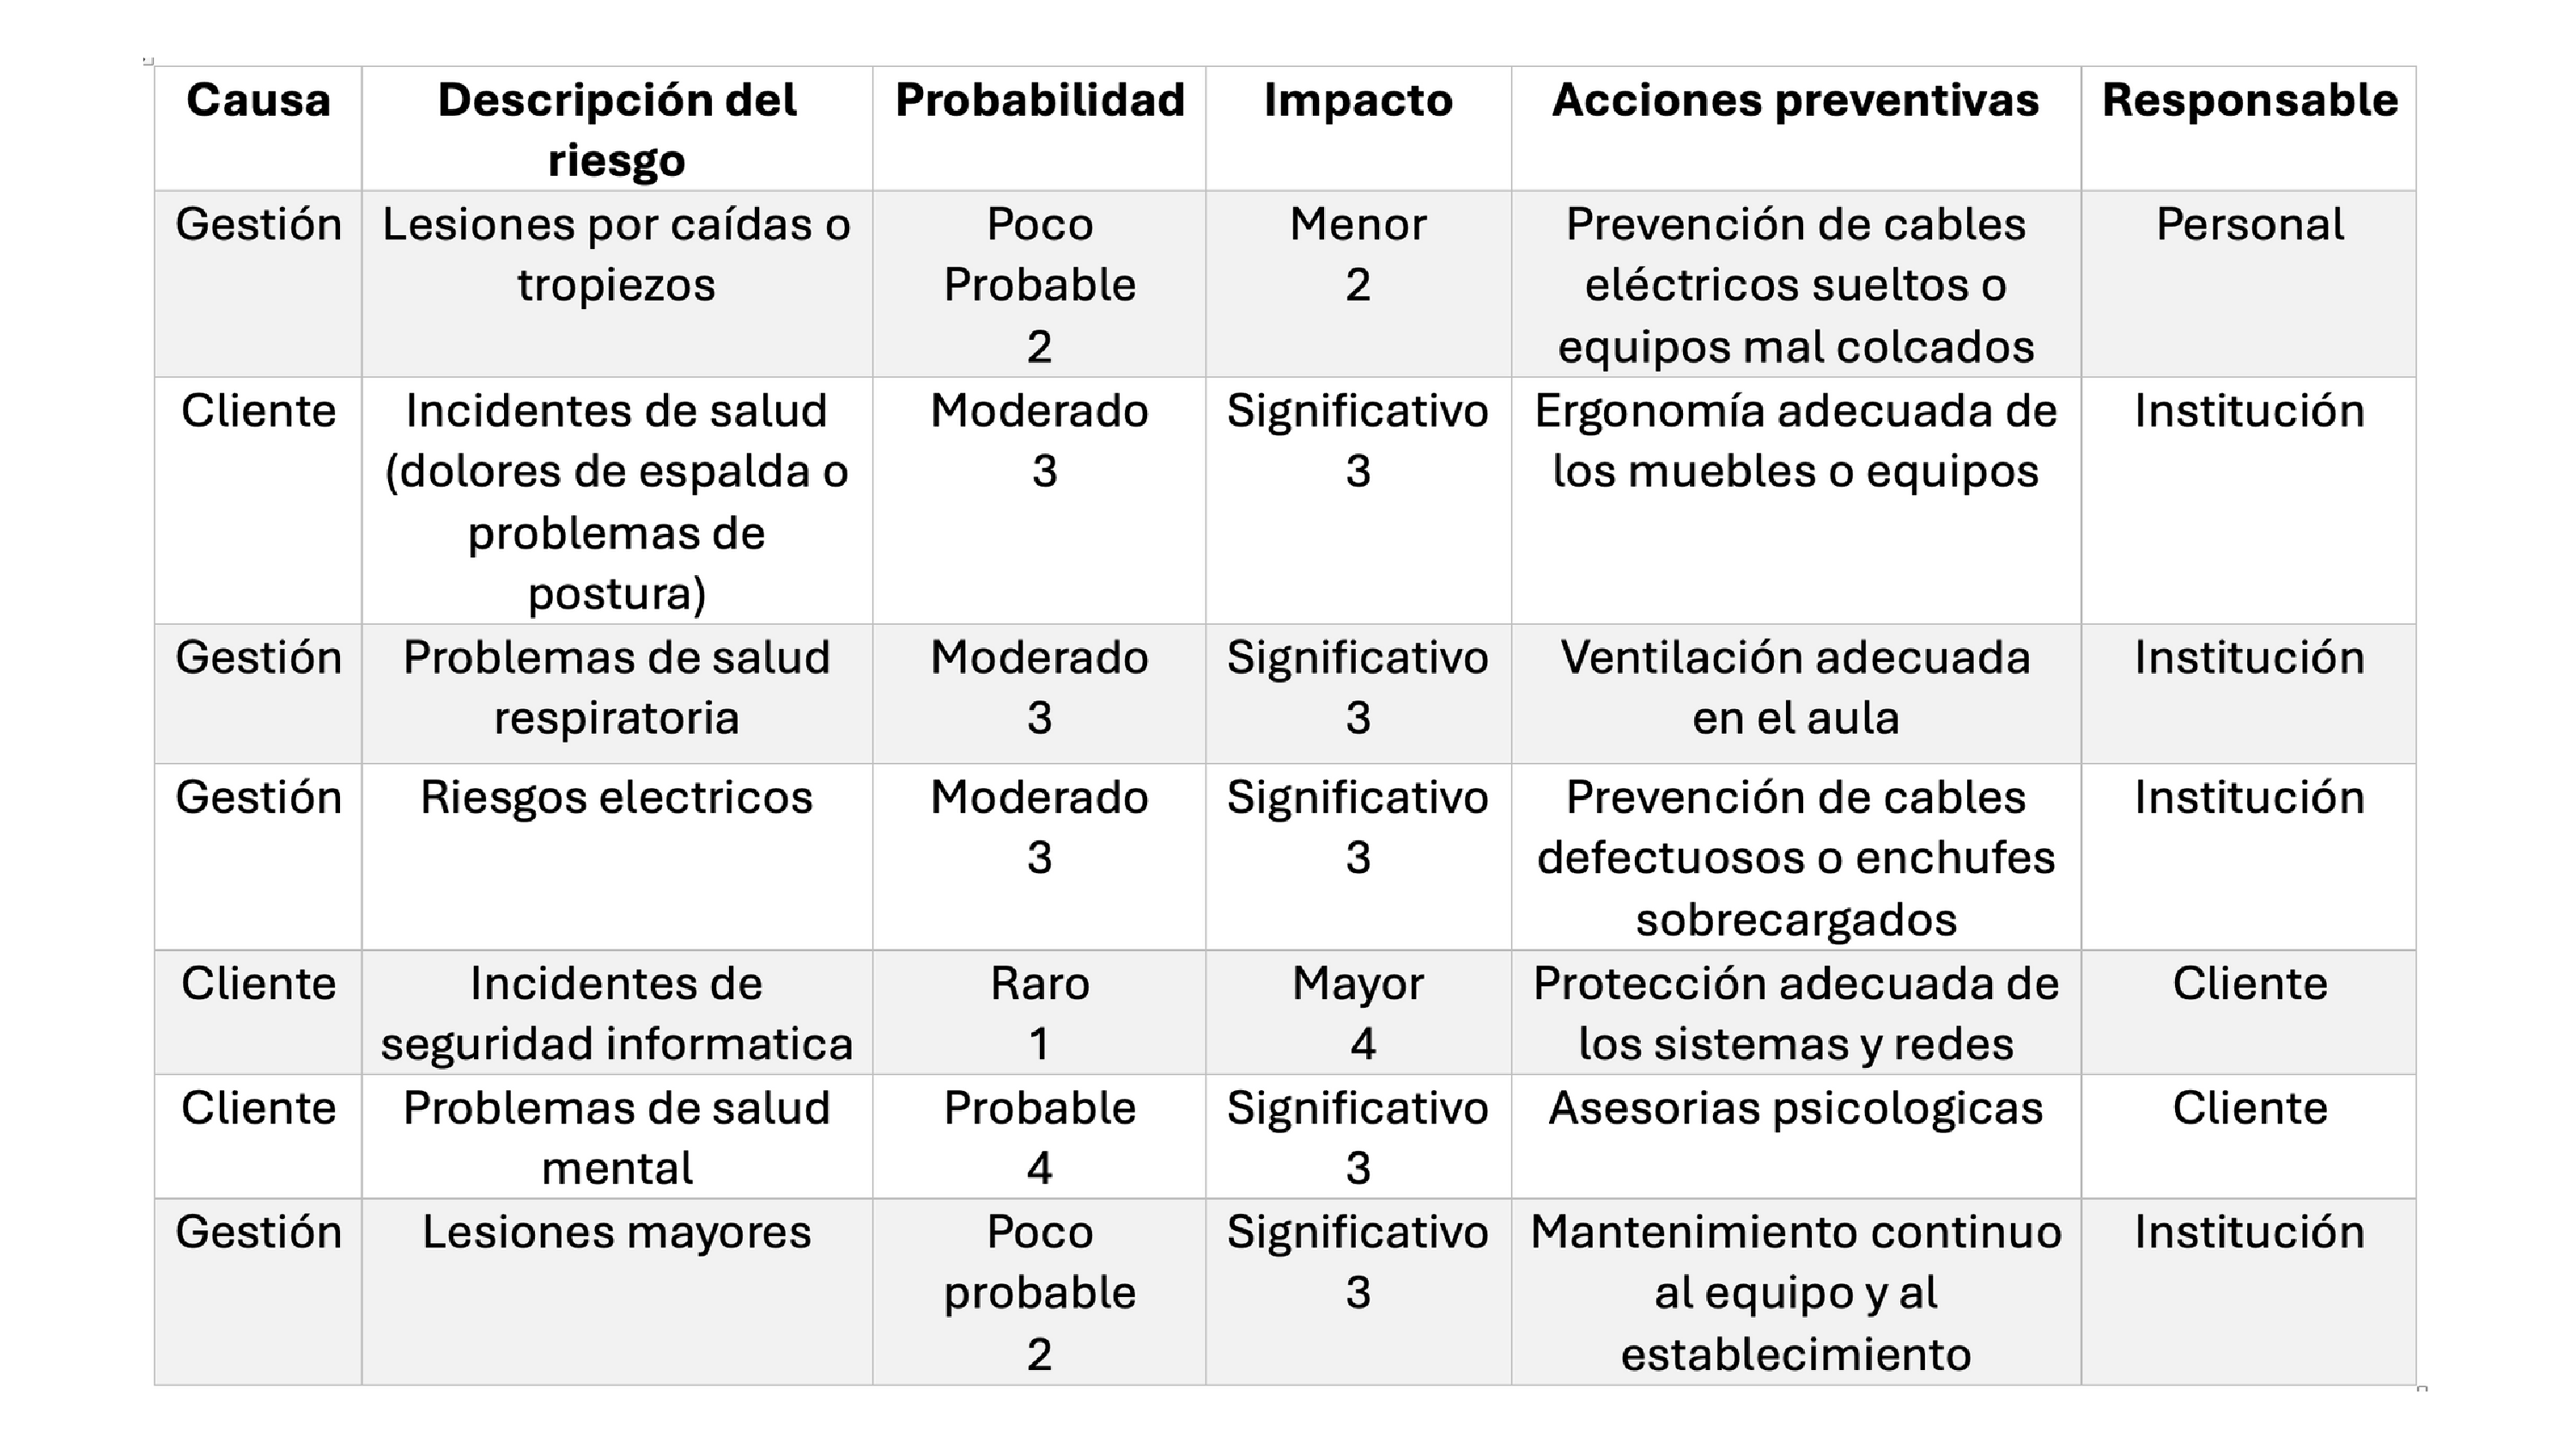
\includegraphics[scale=0.17]{15/img/talaRiesgosInternos.pdf}
        \caption{Descripción de los riesgos al realizar las actividades más comunes y de riesgo dentro del aula.}
        \label{fig:tablaRiesgosInternos}
    \end{figure}
    
    % 
    \subsubsection{Riesgos externos}
    % 
    Por otro lado, el riesgo operativo externo se define como la probabilidad de que la empresa experimente interrupciones o pérdidas debido a factores fuera de su control que afectan su funcionamiento. Específicamente, se refiere a los riesgos que surgen del entorno externo de la empresa, tales como cambios en las políticas gubernamentales, desastres naturales y situaciones de inseguridad en el área circundante. Estos riesgos provienen de influencias externas y no de deficiencias internas en los procesos o funciones de la empresa.
    
    \begin{figure}[H]
        \centering
        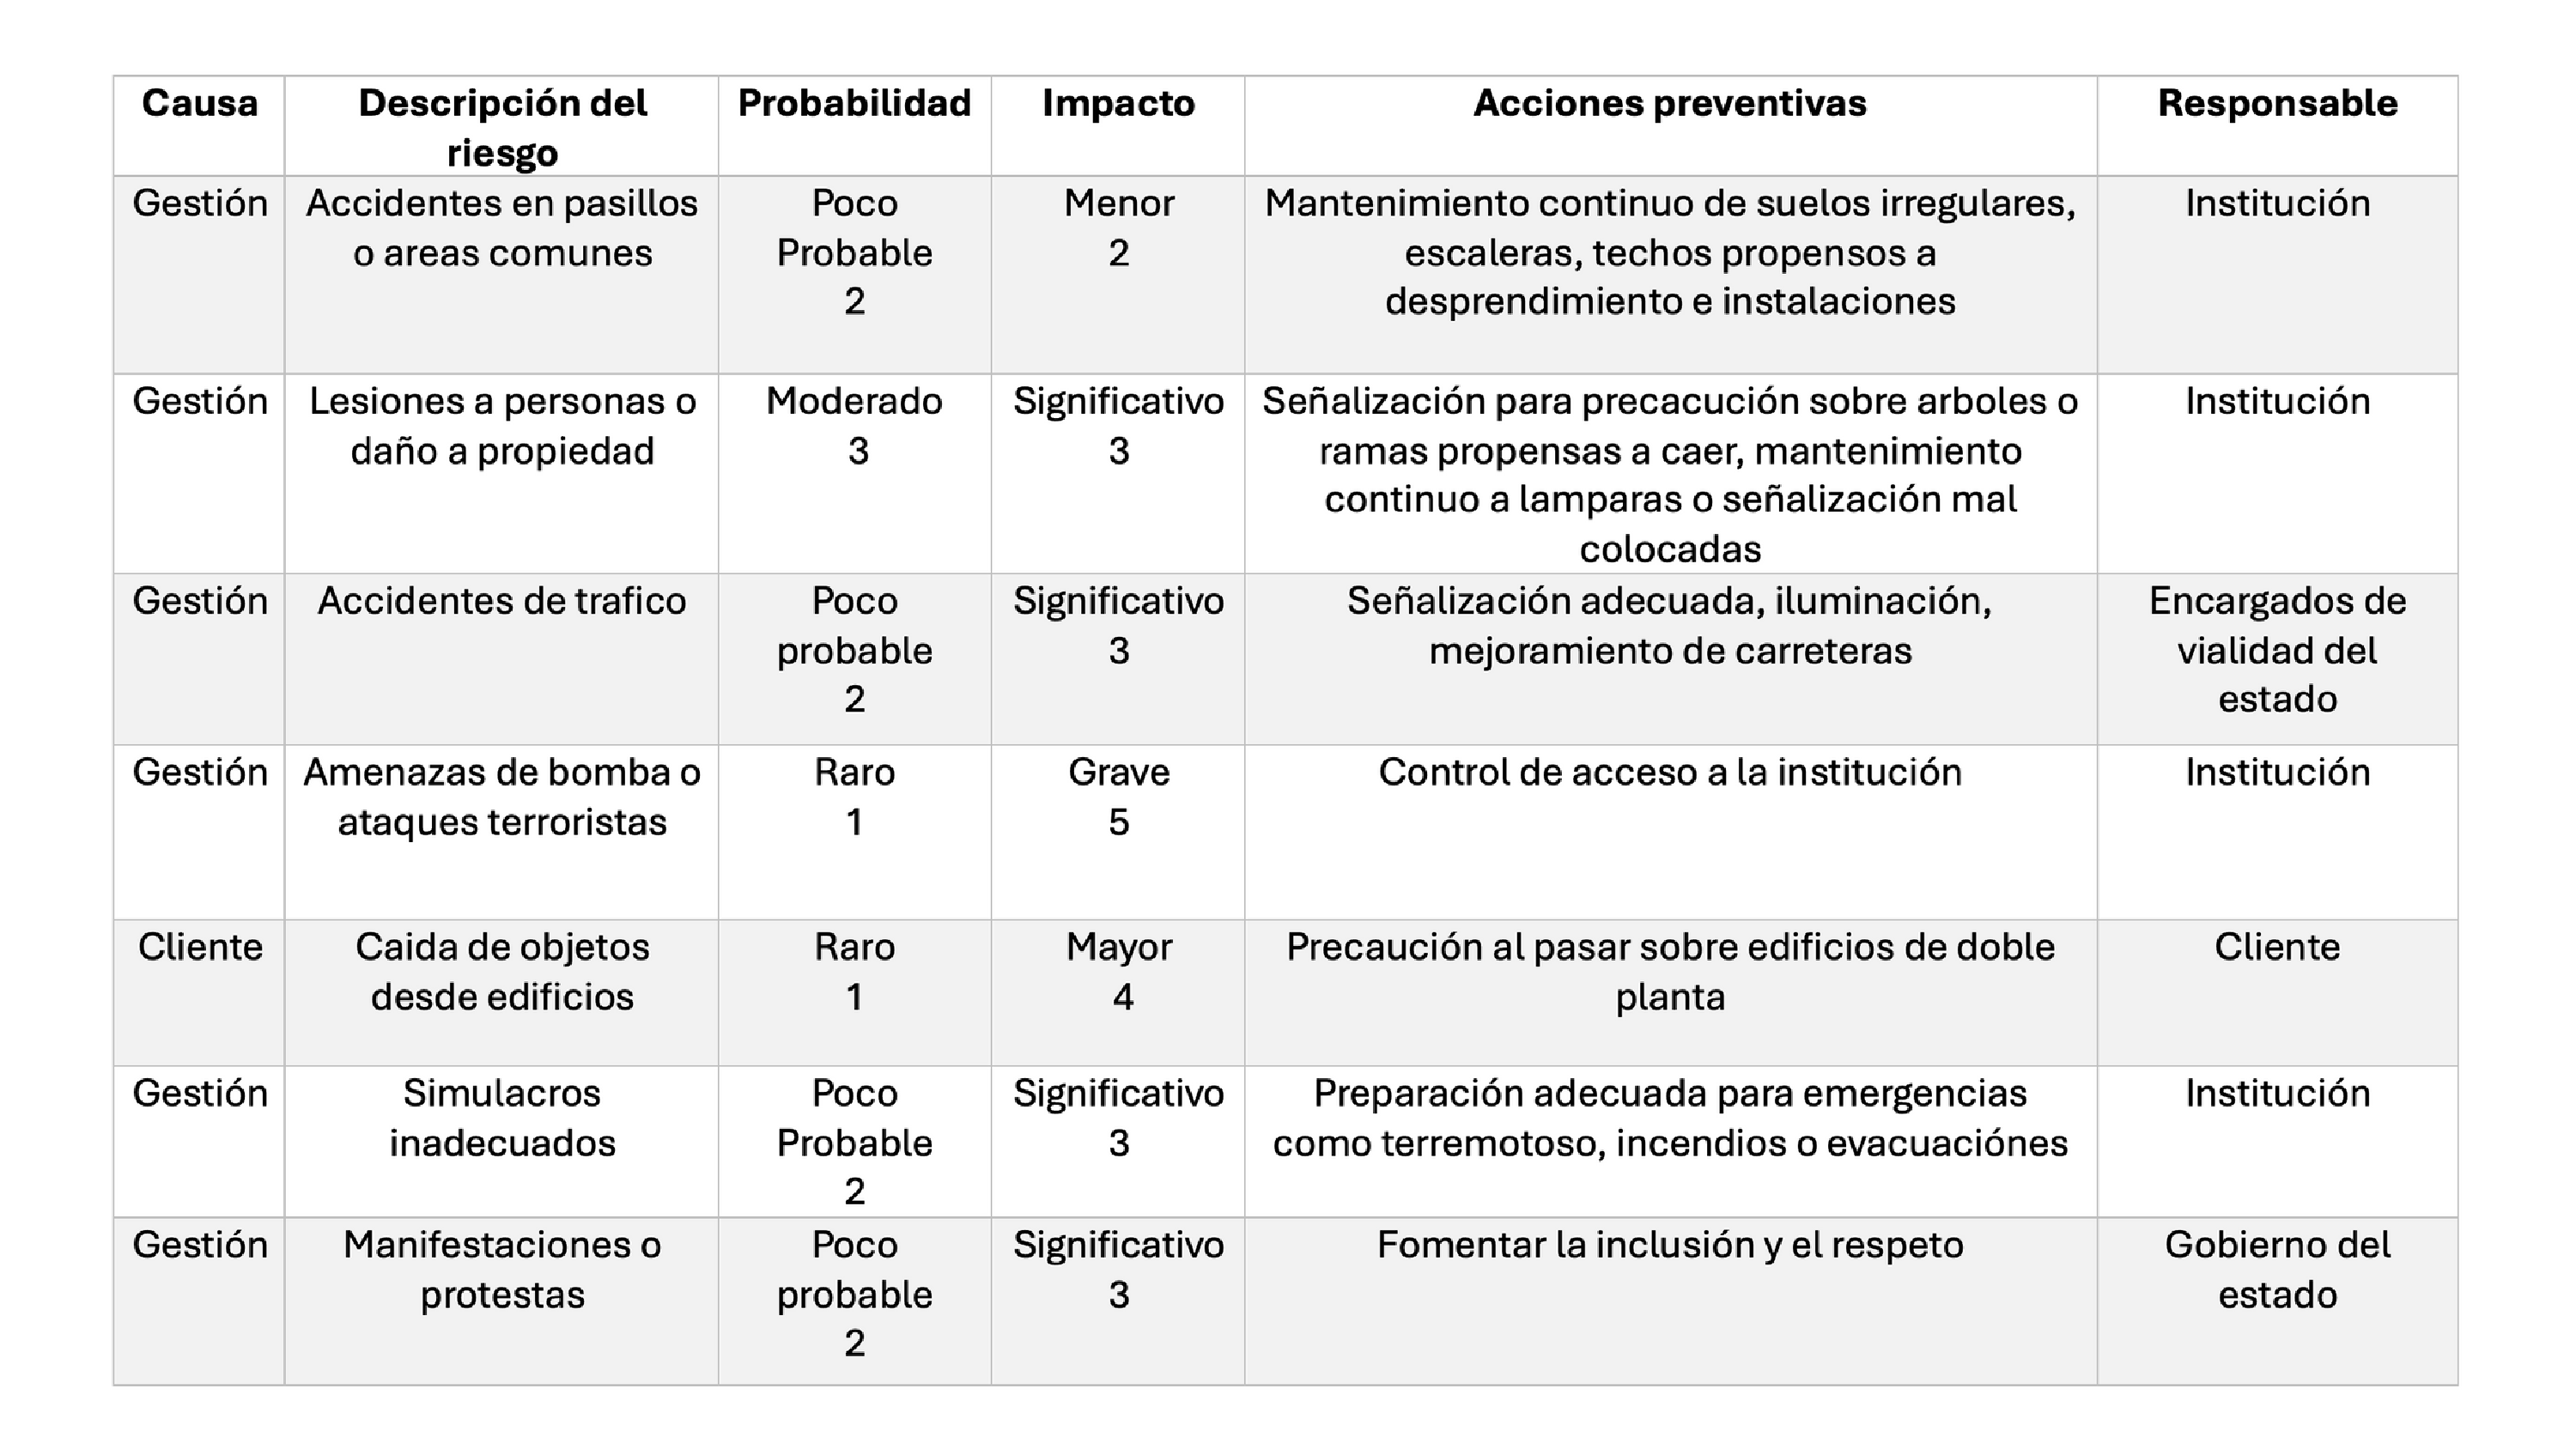
\includegraphics[scale=0.17]{15/img/talaRiesgosExternos.pdf}
        \caption{Descripción de los riesgos externos.}
        \label{fig:tablaRiesgosExternos}
    \end{figure}
    
    % 
    \subsubsection{Programa de actividades de prevención y auxilio}
    % 
    Identificamos las diversas medidas que se implementarán en respuesta a la ocurrencia de un riesgo interno o externo. Además, describimos las actividades de preparación y las disposiciones que se llevan a cabo de manera anticipada en el Instituto Tecnológico de Querétaro (ITQ) para prevenir riesgos.
    % 
    \subsubsection{Plan de acción}
    %
    Conjunto unitario de instrucciones estratégicas que habilita al ITQ para realizar una amplia gama de funciones, desde abordar problemas internos hasta gestionar riesgos externos de manera efectiva. Este plan detalla las medidas específicas que se deben tomar en caso de que surjan riesgos, tanto dentro como fuera de la institución. Incluye protocolos de respuesta claros, asignación de responsabilidades, recursos necesarios y un cronograma para su implementación. Además, el plan de acción se desarrolla de manera proactiva, mediante la identificación anticipada de posibles riesgos y la adopción de medidas preventivas para mitigar su impacto. Este enfoque proactivo garantiza que el ITQ esté preparado para hacer frente a cualquier desafío que pueda surgir, protegiendo así los intereses y la seguridad de la comunidad universitaria.
    
    \begin{figure}[H]
        \centering
        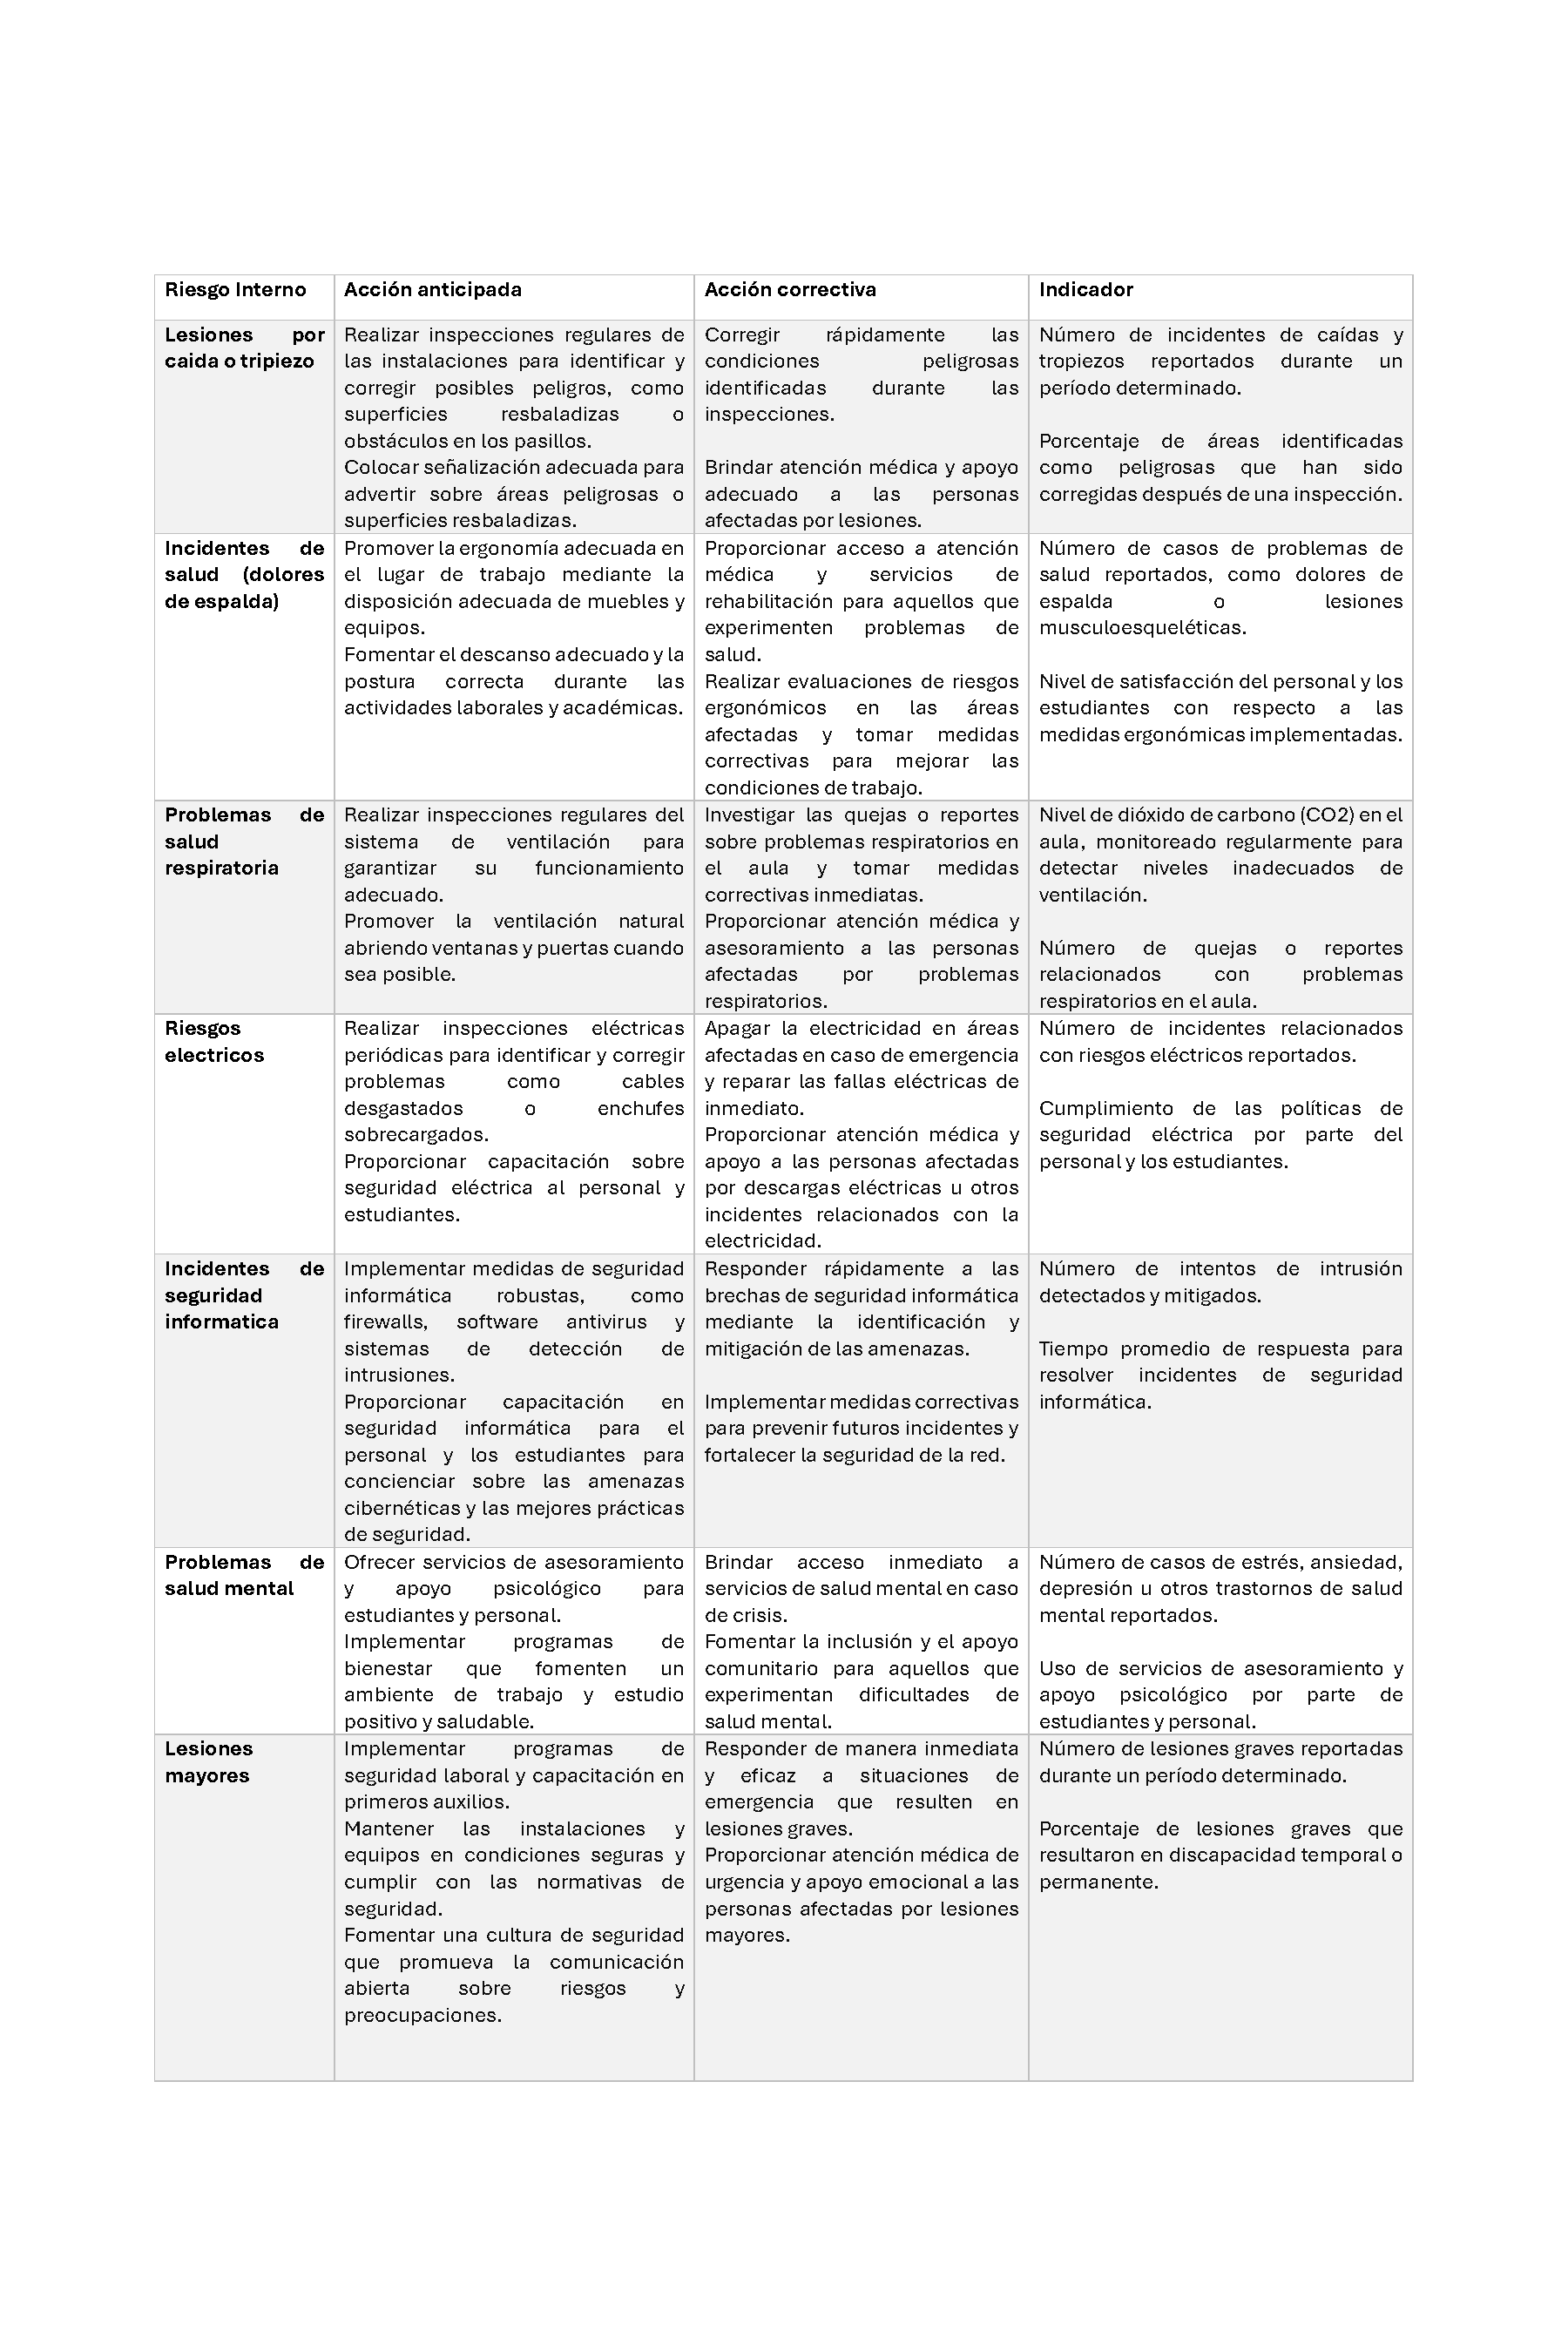
\includegraphics[scale=0.3]{15/img/tablaPlanDeAccionRiesgosInternos.pdf}
        \caption{Descripción de las acciones anticipadas y correctivas ante un riesgo interno.}
        \label{fig:tablaPlanDeAccionRiesgosInternos}
    \end{figure}
    
    \begin{figure}[H]
        \centering
        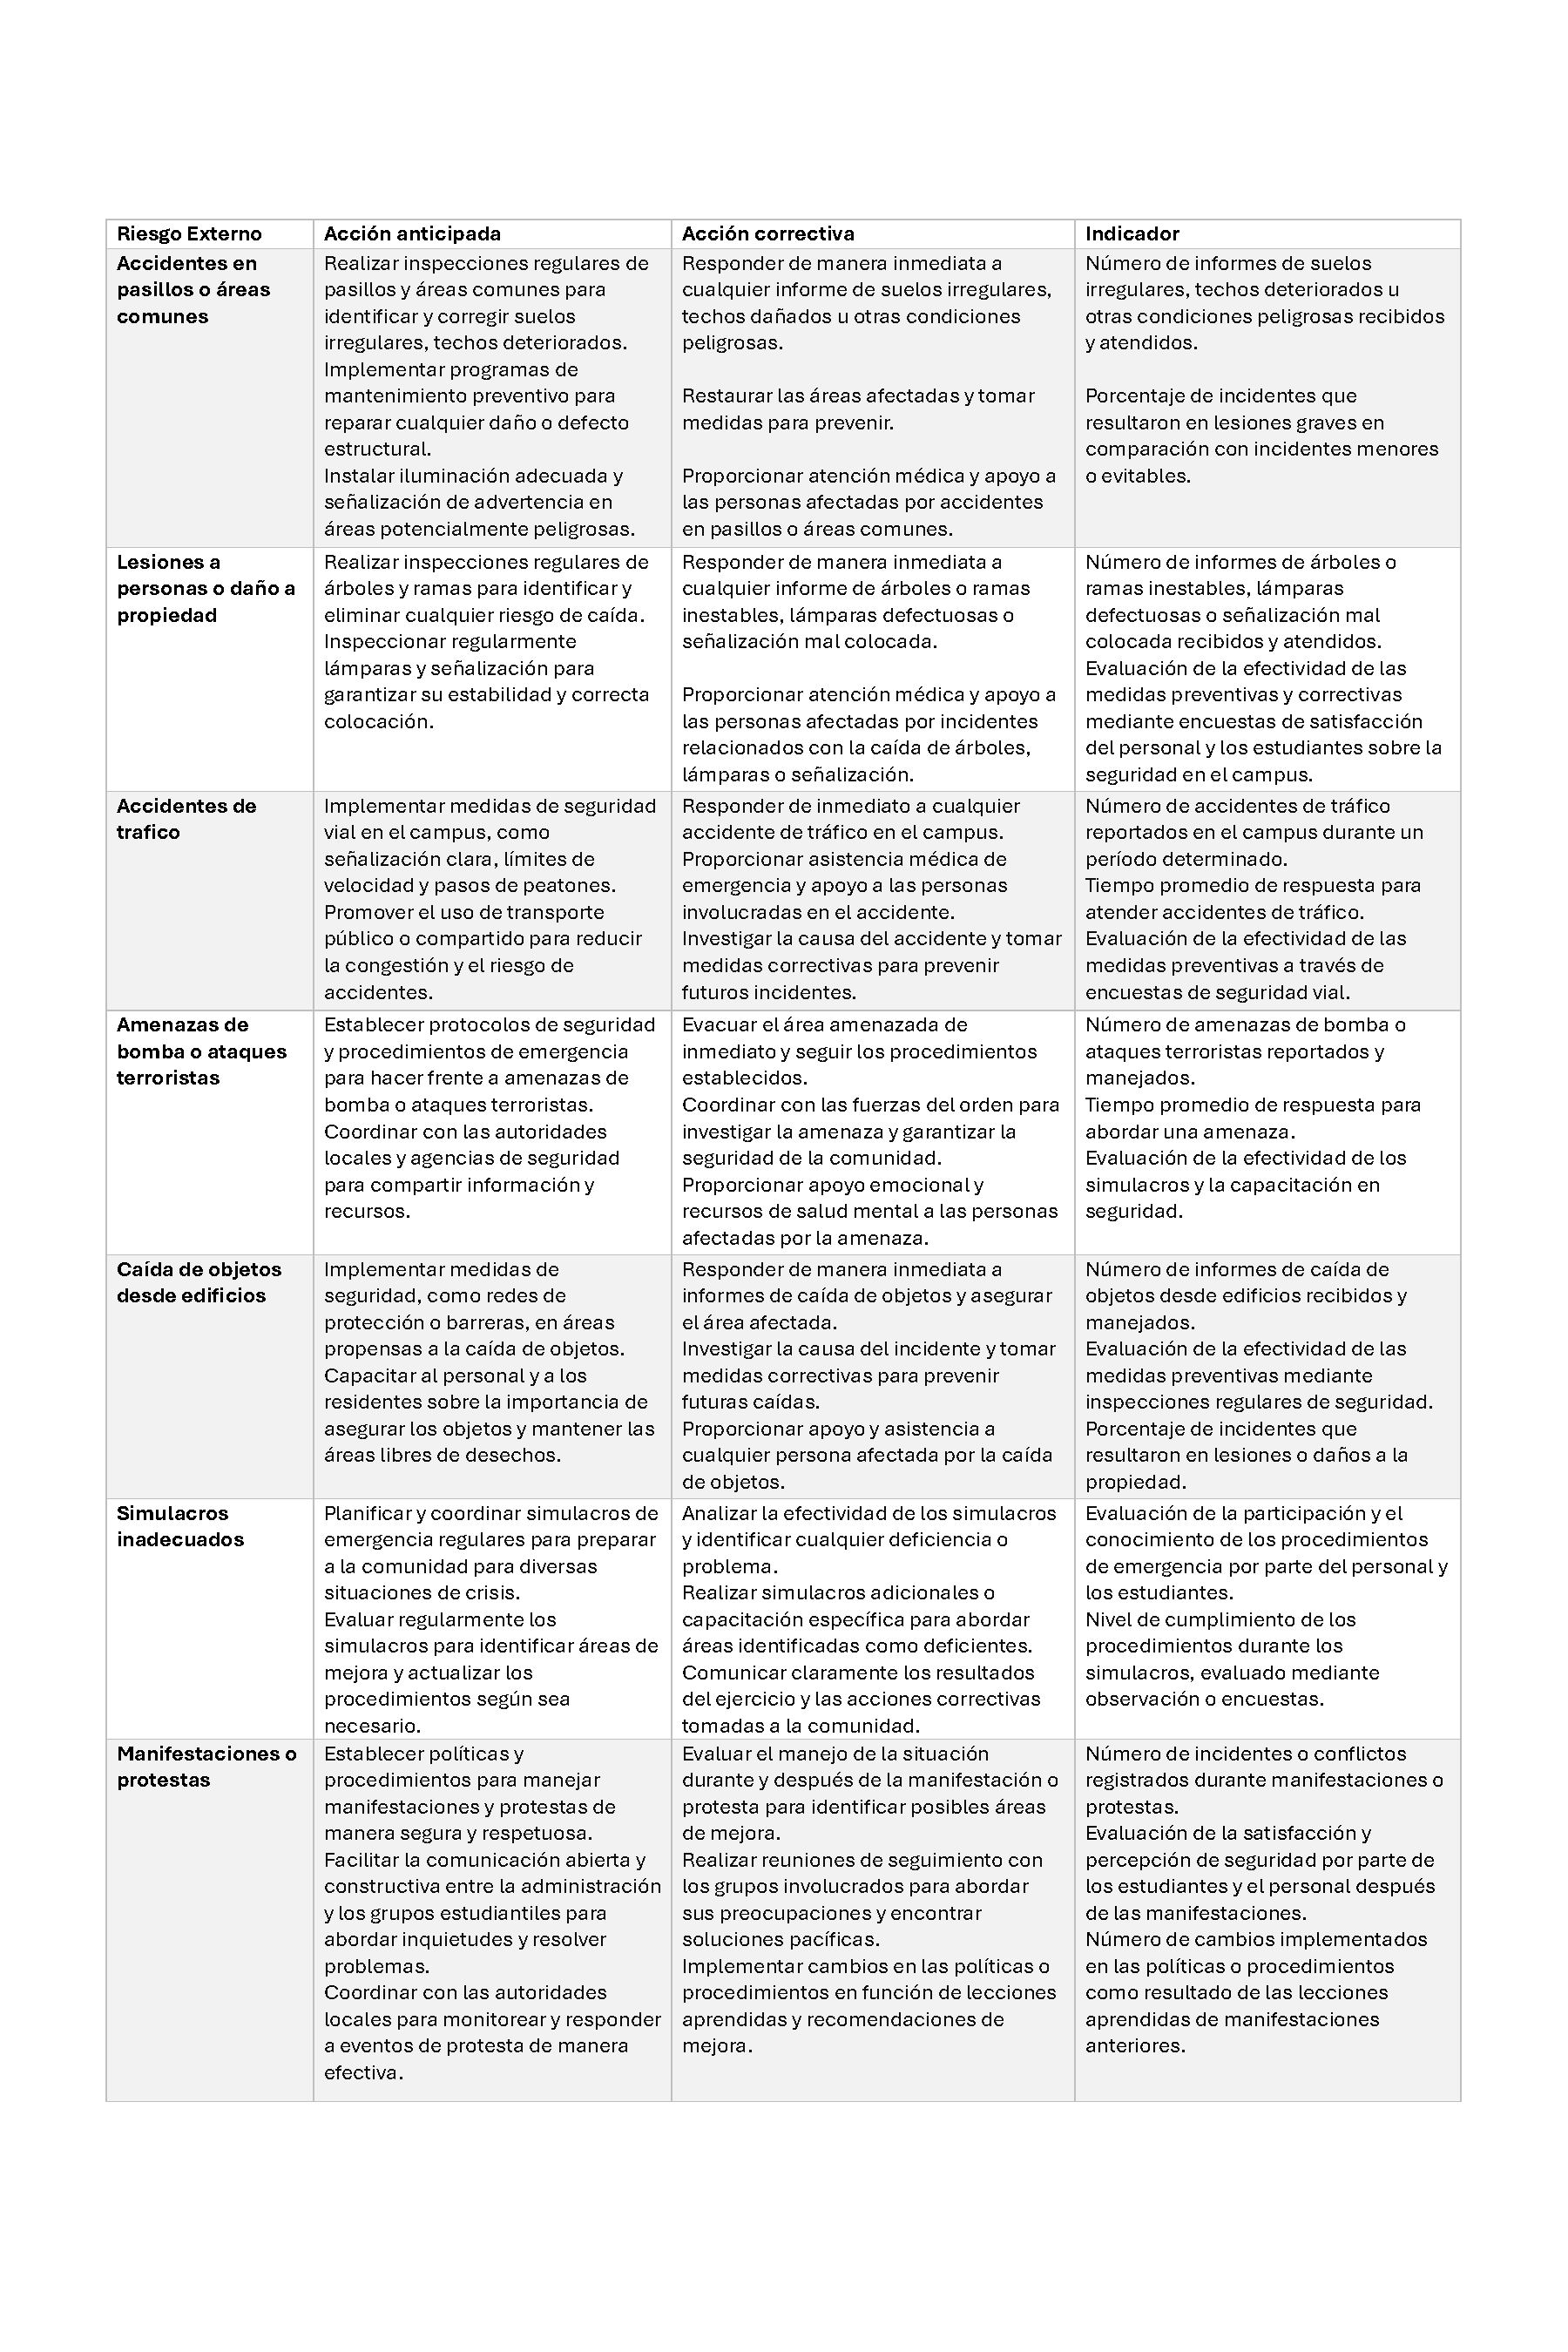
\includegraphics[scale=0.3]{15/img/tablaPlanDeAccionRiesgosExternos.pdf}
        \caption{Descripción de las acciones anticipadas y correctivas ante un riesgo externos.}
        \label{fig:tablaPlanDeAccionRiesgosExternos}
    \end{figure}
    
    \subsubsection{Identifiación de capacidades.}
    % 
    %
    \subsubsection{Plano de localización de recursos.}
    % 
    %
    \subsubsection{Identifiación de apoyos externos.}
    % 
    \begin{figure}[H]
        \centering
        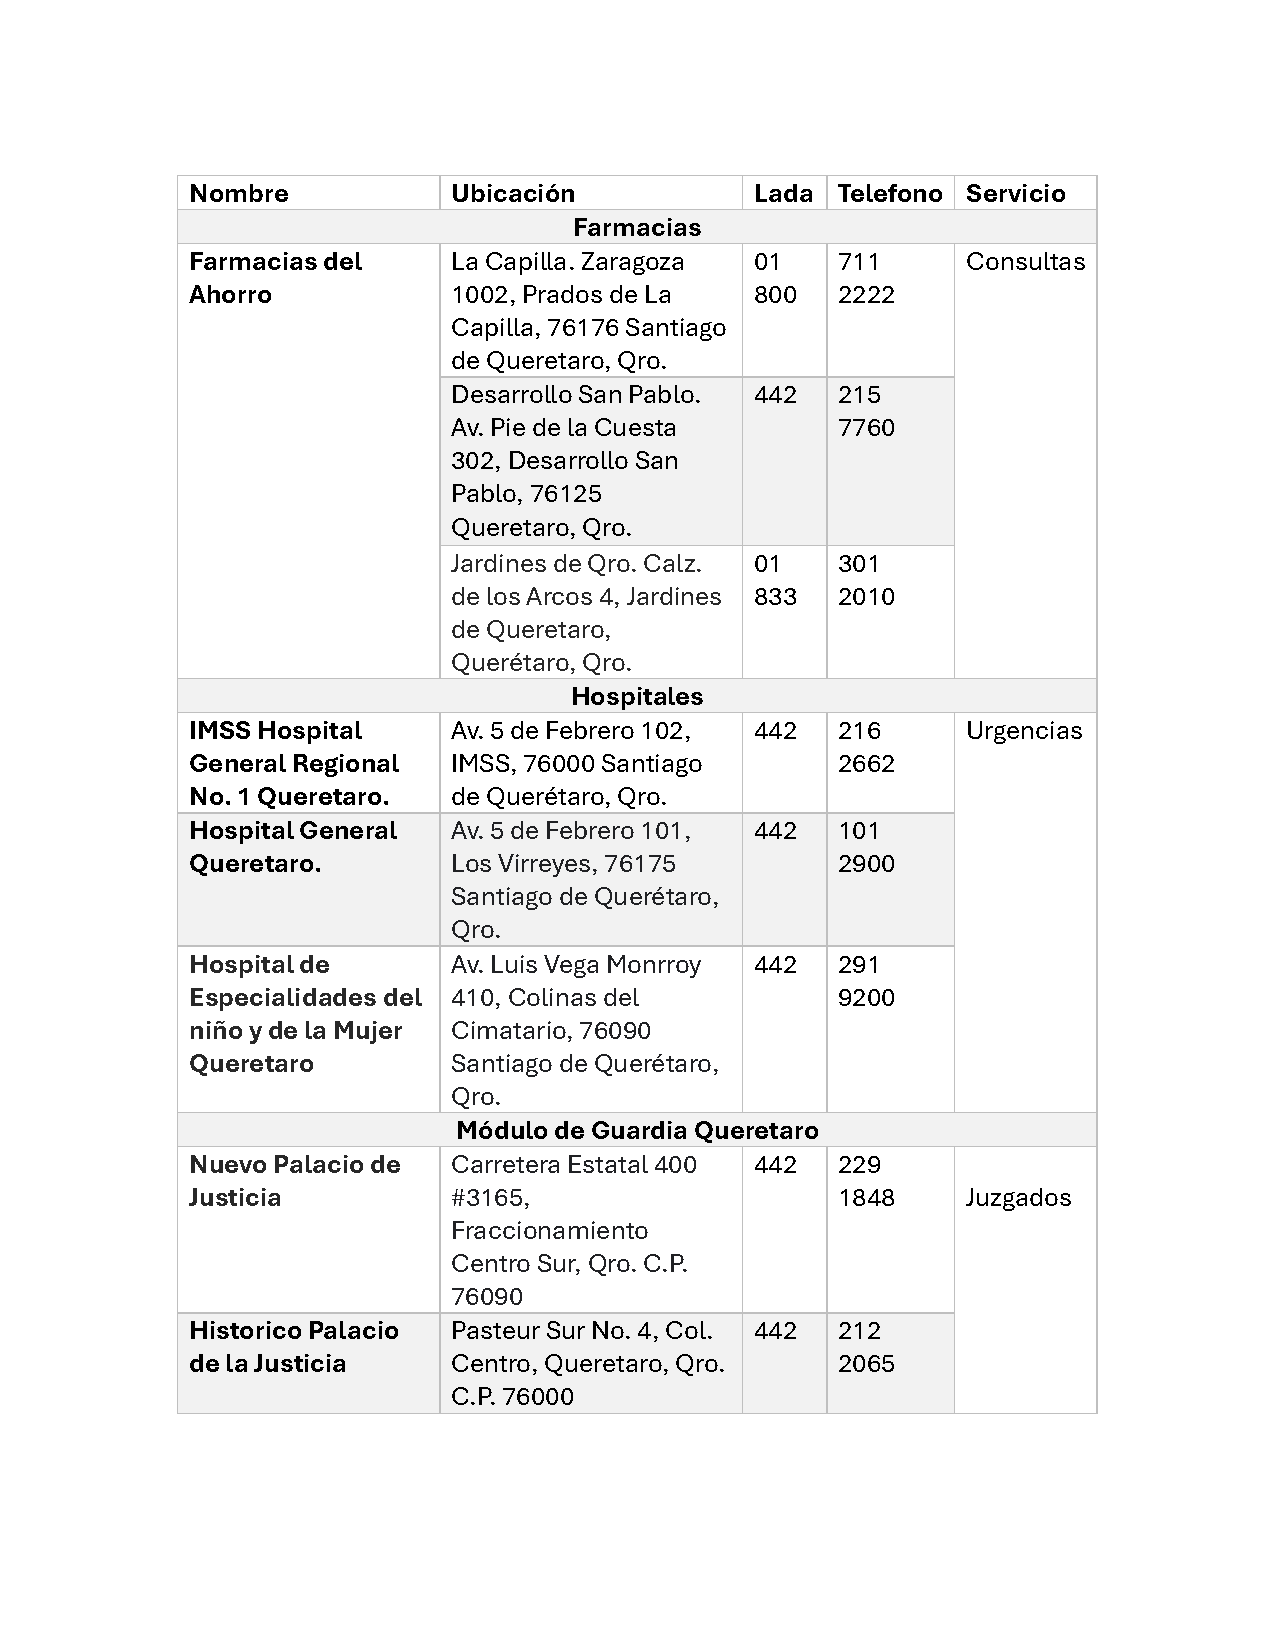
\includegraphics[scale=0.4]{15/img/tablaApoyosExternos.pdf}
        \caption{Lugares que servirán de apoyo en un situación de emergencia.}
        \label{fig:tablaApoyosExternos}
    \end{figure}
    %
    \subsubsection{Identifiación de puntos de reunión.}
    % 
    \begin{figure}[H]
        \centering
        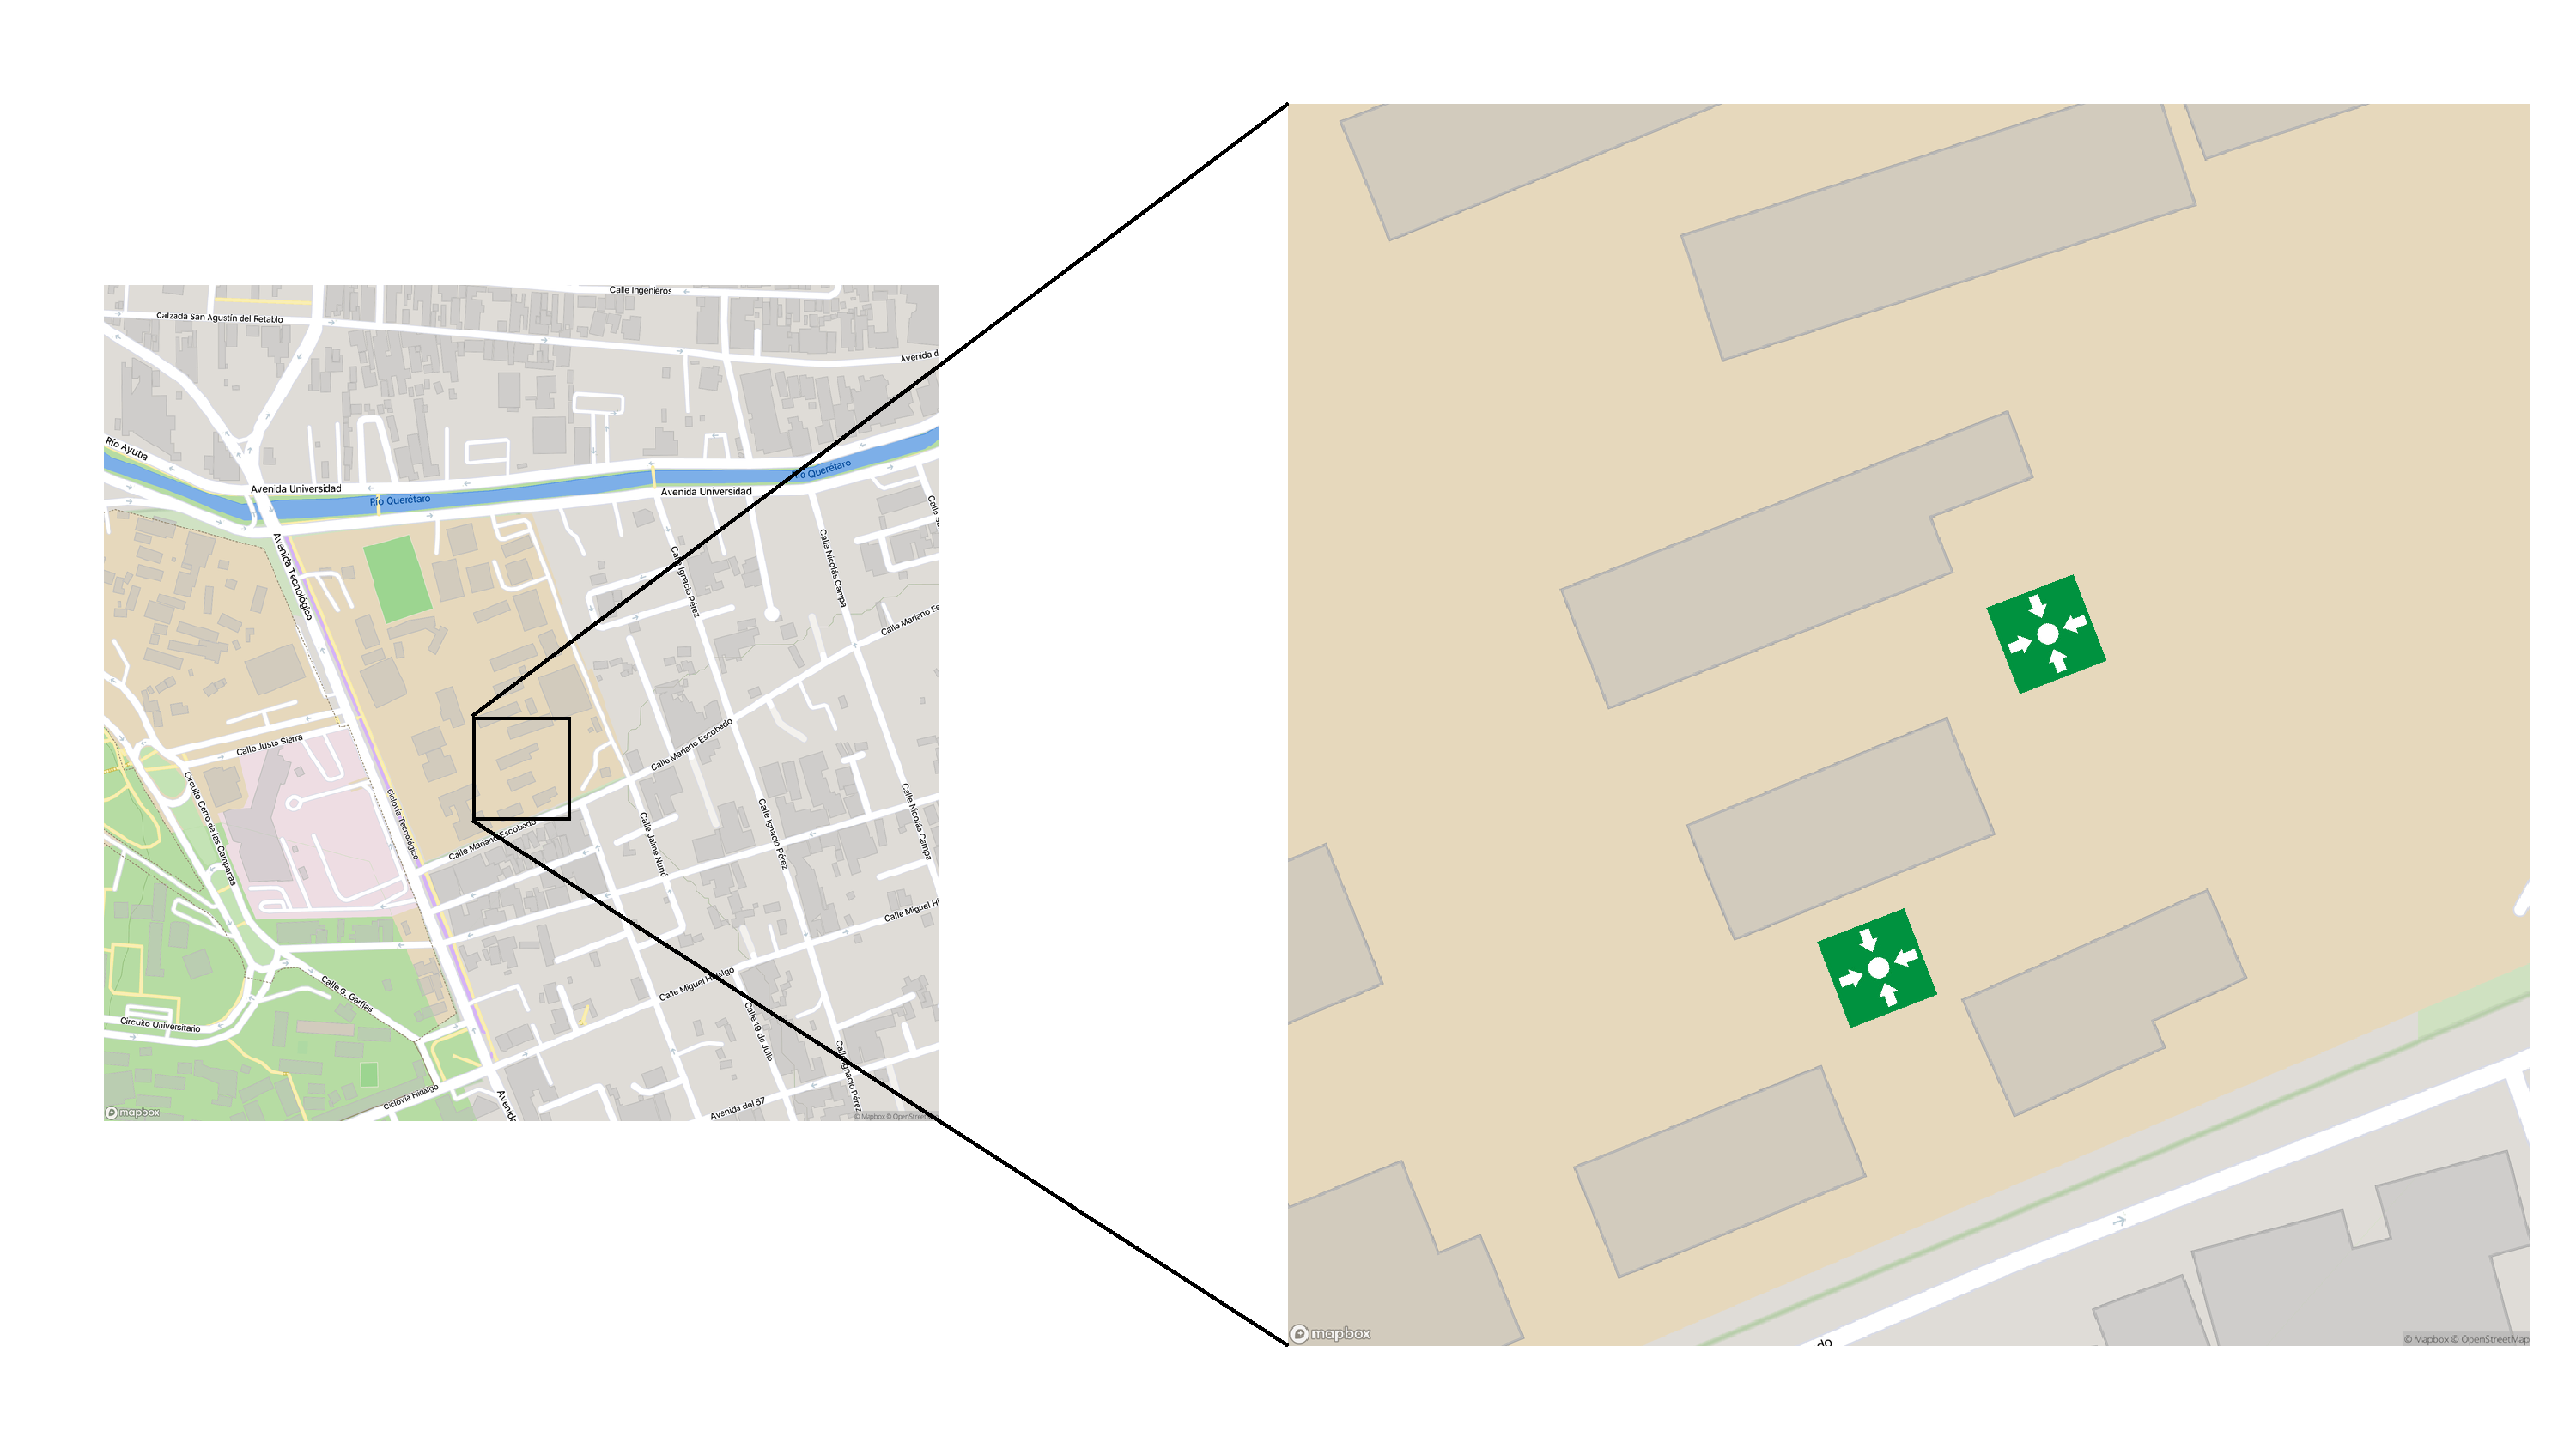
\includegraphics[scale=0.15]{15/img/mapaPuntosDeReunion.pdf}
        \caption{Zona segura en caso de una evacuación de emergencia.}
        \label{fig:mapaPuntosDeReunion}
    \end{figure}
    %
    \subsubsection{Brigada de evacuación.}
    % 
    \begin{figure}[H]
        \centering
        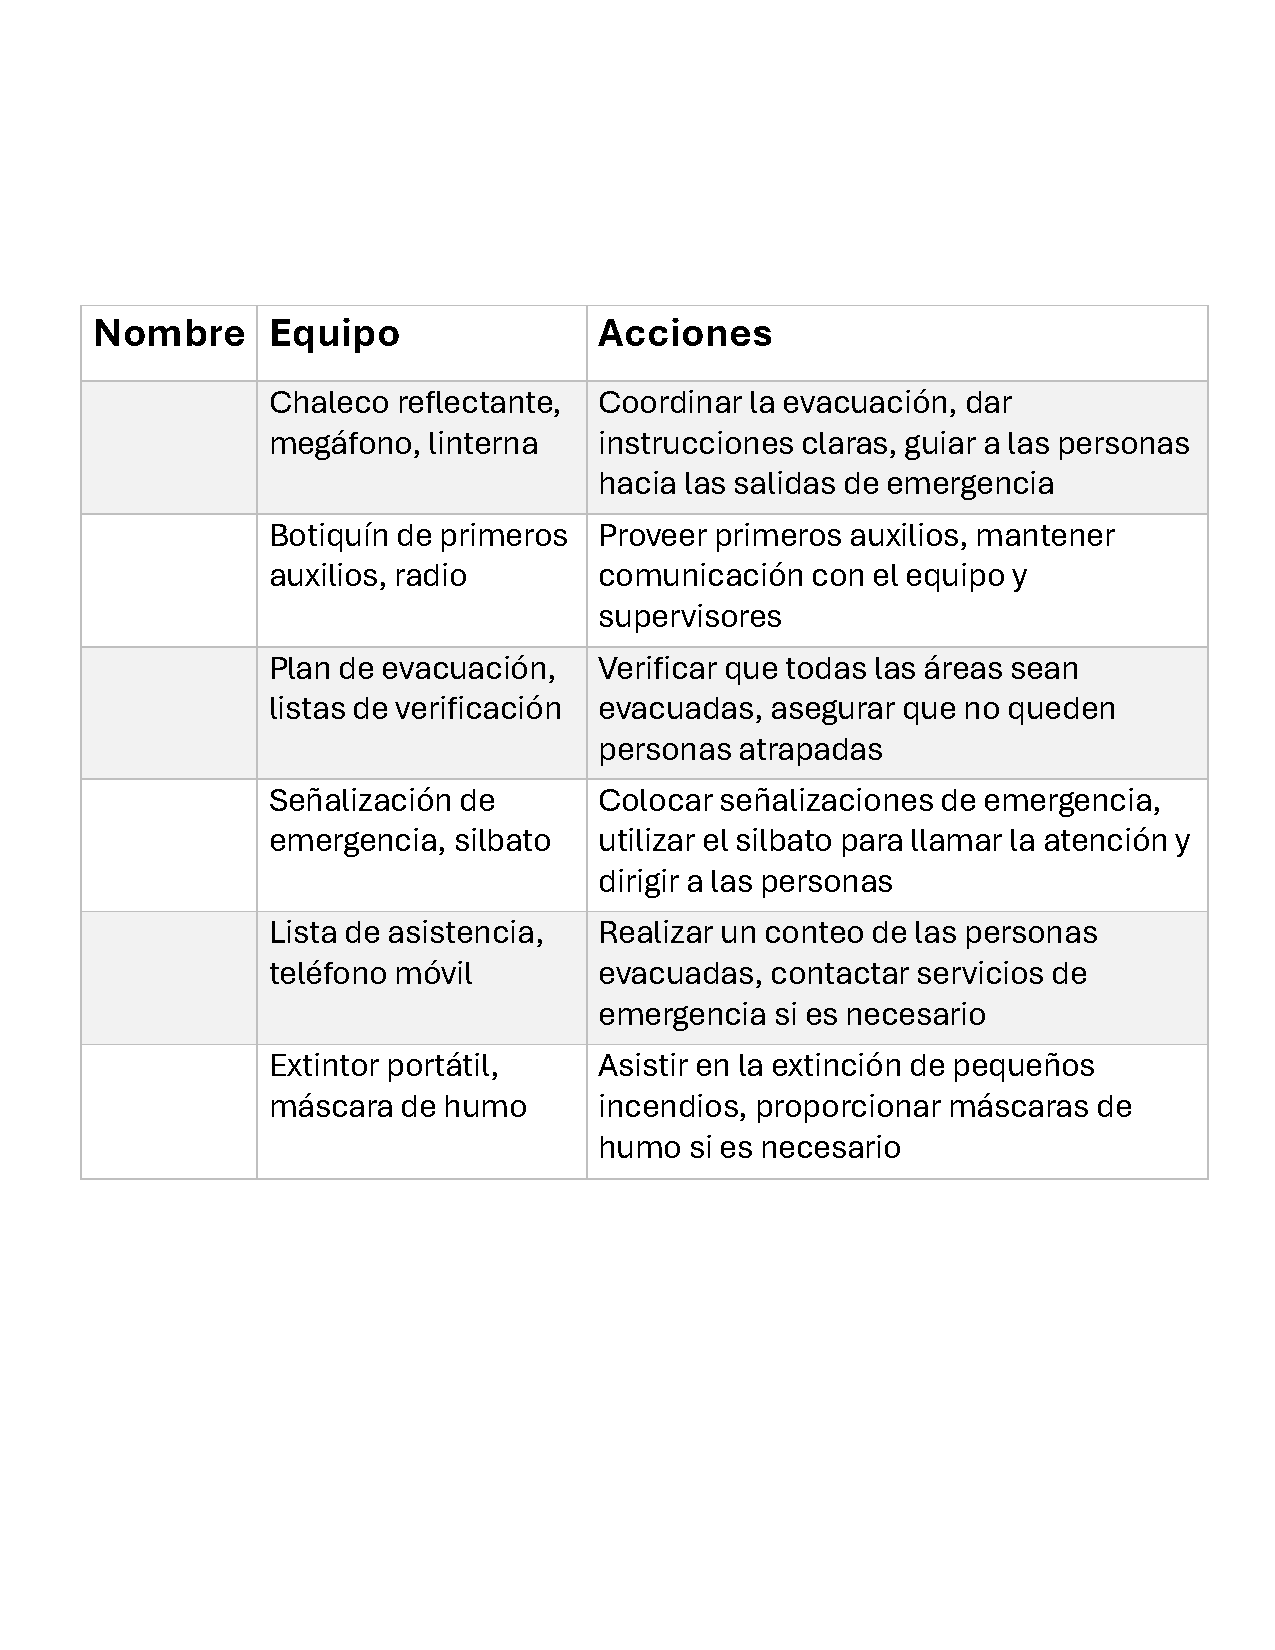
\includegraphics[scale=0.4]{15/img/tablaBrigadaEvacuacion.pdf}
        \caption{Acciones asignadas a cada integrante del equipo de trabajo en caso de una evacuación de emergencia o repliegue.}
        \label{fig:brigada}
    \end{figure}
    %
    \subsubsection{Directorio telefónico de emergencia.}
    % 
    Directorio telefónico de entidades de respuesta a emergencias y otras organizaciones implicadas en la supervisión y gestión de estas situaciones.
    
    \begin{figure}[H]
        \centering
        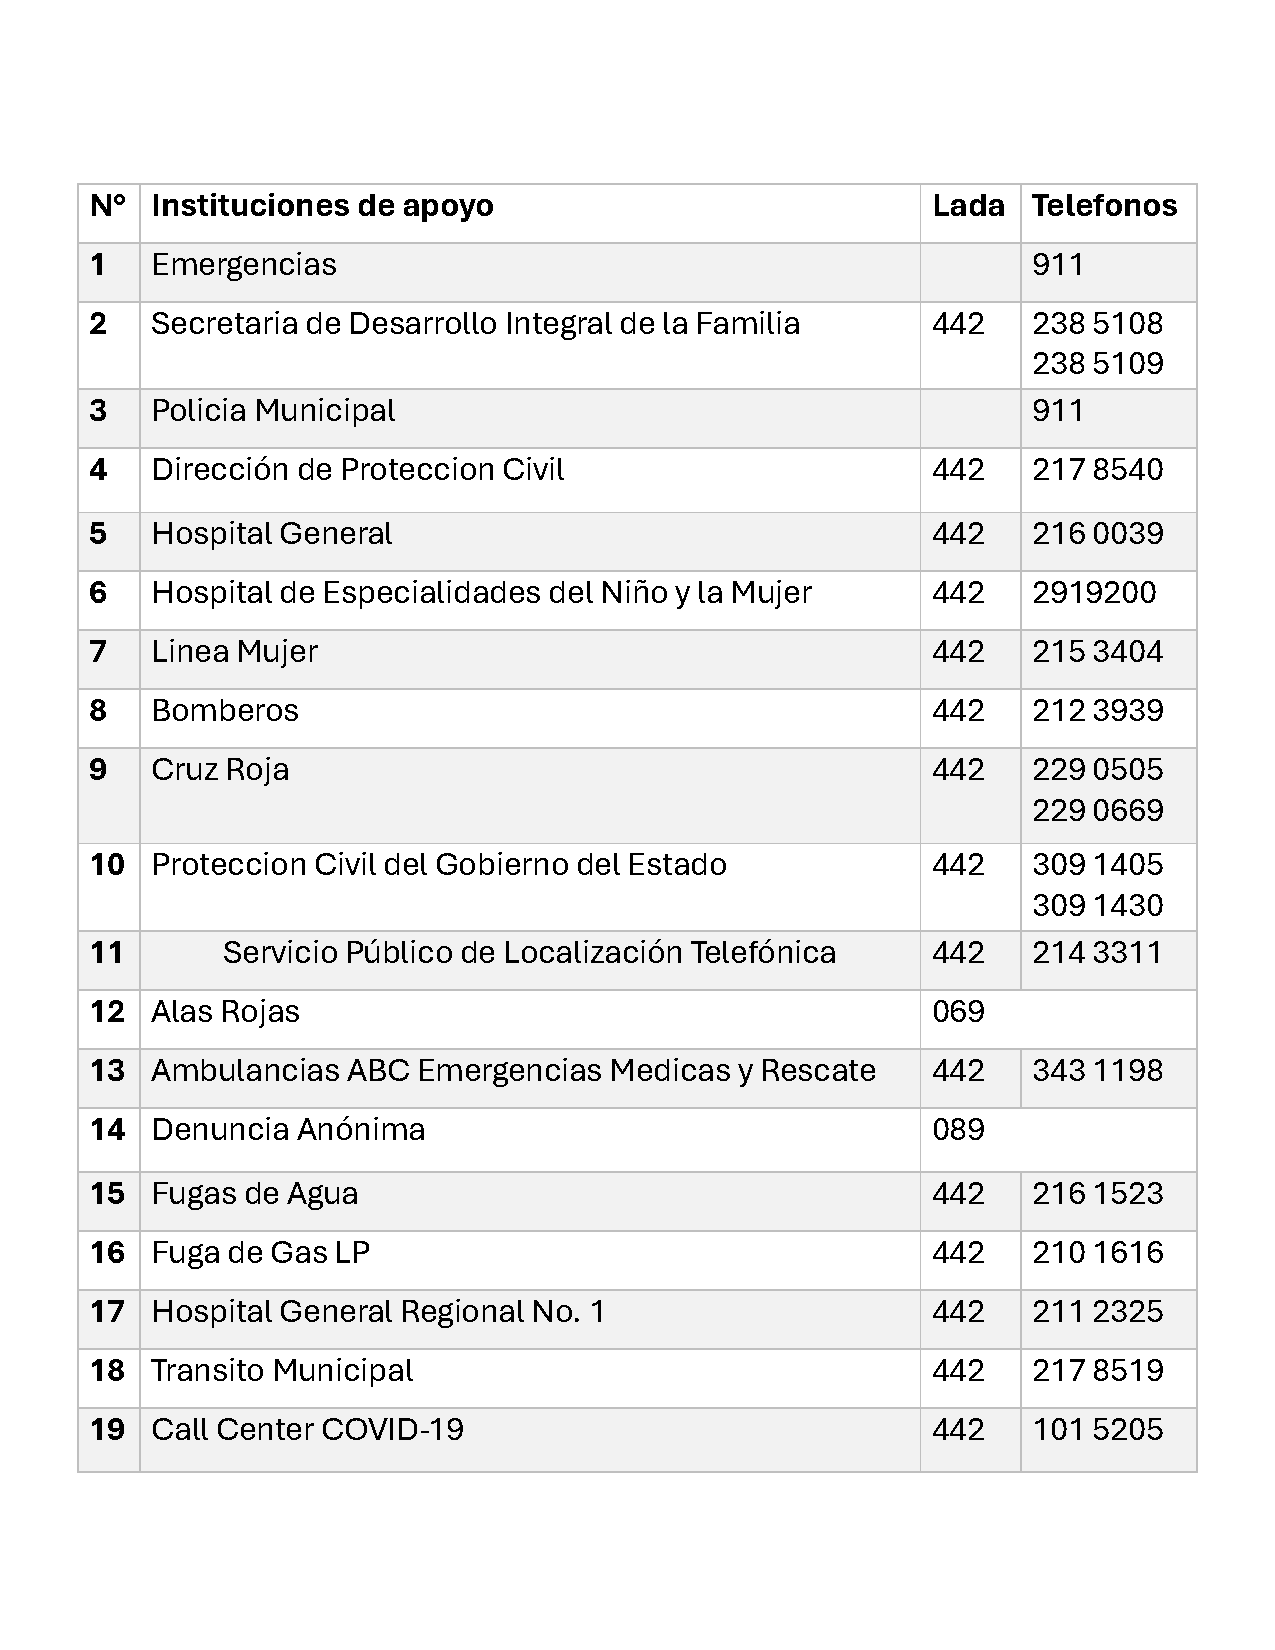
\includegraphics[scale=0.35]{15/img/tablaDirectorioEmergencias.pdf}
        \caption{Números de emergencia.}
        \label{fig:tablaDirectorioEmergencias}
    \end{figure}
    %
    \subsection{Análisis de los métodos, materiales, herramientas e instalación utilizada en la ejecución del ensamble de un circuito electrónico}
    
    \subsubsection{Verificación}
    
    Costos de no calidad.
    % 
    % 
    \subsubsection{Desarrollo del sistema de tiempos predeterminado}
    % 
    Como resultado de lo antes mencionado respecto a los STP, se obtuvieron como resultado la siguiente tabla vease \ref{fig:tablaMTM1-1}
    
    \begin{figure}[H]
        \centering
        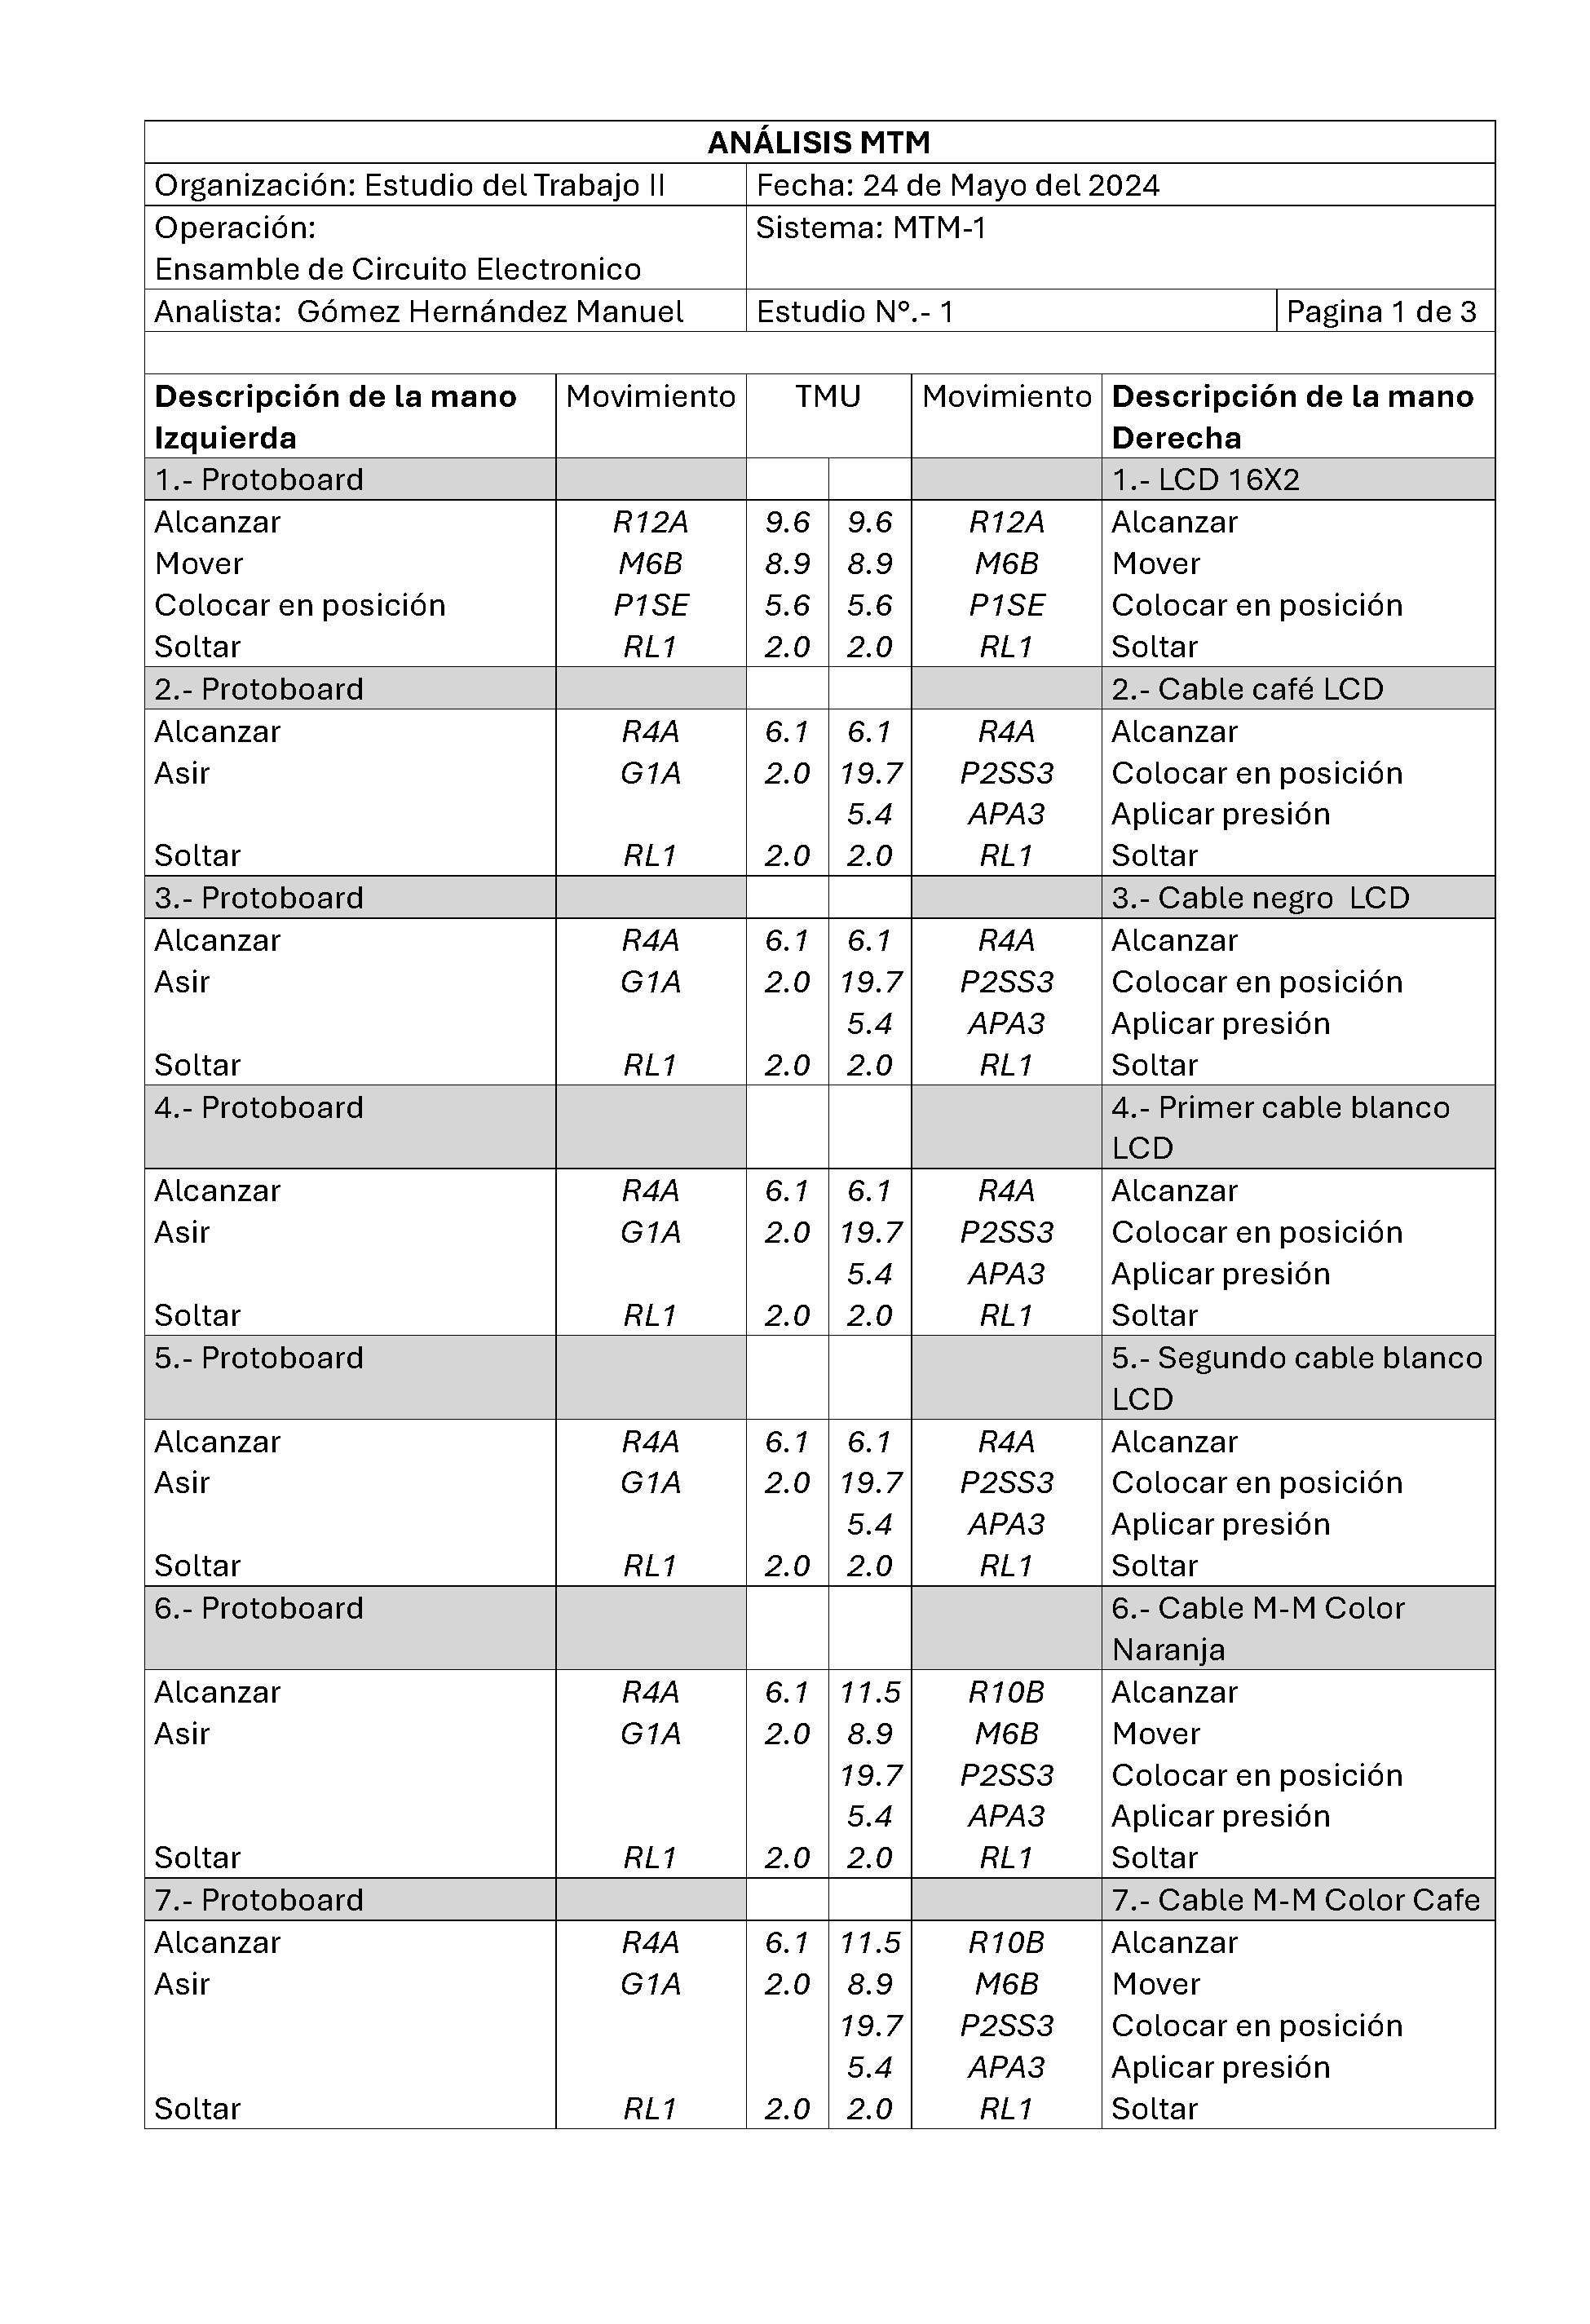
\includegraphics[scale=0.165]{15/img/tablaMTM1-1.pdf}
        \includegraphics[scale=0.165]{15/img/tablaMTM1-2.pdf}
        \includegraphics[scale=0.165]{15/img/tablaMTM1-3.pdf}
        \caption{Hoja de análisis de métodos resultante en base a su  metodología.}
        \label{fig:tablaMTM1-1}
        \end{figure}
    
    % 
    \subsubsection{Desarrollo del muestreo del trabajo}
    % 
    % 
    \subsubsection{Corrección por balanceo de procesos}
    % 
    % 
    \subsubsection{Datos estándar continuos y discretos}
    % 
    % 
    \subsection{Diseño de la forma más económica de realizar el trabajo}
    % 
    
        \begin{figure}[H]
        \centering
        \includegraphics[scale=0.165]{15/img/tablaEconomicaTrabajo.pdf}
        \caption{Tabla de comparación de materiales}
        \label{fig:tablaEconomicaTrabajo}
        \end{figure}
    % 
    \subsection{Normalización de los métodos, materiales, herramientas e instalaciones}
    
    % 
    % 
    \subsection{Determinación del tiempo estándar para que una persona competente realice el trabajo con marcha normal}
    En relacion a lo antes mencionado sobre el tiempo estandar, se obtuvo como resultado la siguientes tablas, donde se utilizo la tabola Bimanual para la obtencion de los movimientos \ref{fig:tablaBimanual} y obtener el tiempo ciclo en base a dichos movimientos tanto individualmente \ref{fig:tiemposCiclos} como de 12 muestras \ref{fig:tiempoCicloTodos}, de igual forma para la obtención del tiempo estandar sus holguras o suplementos \ref{fig:calculoHolguras} para asi la obtención de su tiempo estandar \ref{fig:tiempoEstandarCalculo} teniendo como resultado un tiempo de 3.56 minutos.
    
        \begin{figure}[H]
        \centering
        \includegraphics[scale=0.15]{15/img/diagramaBimanualEnsamble.pdf}
        \includegraphics[scale=0.15]{15/img/diagramaBimanualEnsamble2.pdf}    \includegraphics[scale=0.15]{15/img/diagramaBimanualEnsamble3.pdf}
        \caption{Tabla Bimanual}
        \label{fig:tablaBimanual}
        \end{figure}
        
        \begin{figure}[H]
        \centering
        \includegraphics[scale=0.165]{15/img/tiemposCiclos.pdf}
        \caption{Tiempo Ciclo Individual en base a los movimeintos de la Tabla Bimanual.}
        \label{fig:tiemposCiclos}
        \end{figure}
    
    
        \begin{figure}[H]
        \centering
        \includegraphics[scale=0.2]{15/img/tiemposCiclosTodos.pdf}
        \includegraphics[scale=0.2]{15/img/tiemposCiclosTodos2.pdf}
        \caption{Tiempo ciclo de 12 muestras}
        \label{fig:tiempoCicloTodos}
        \end{figure}
    
        
    \begin{figure}[H]
        \centering
        \includegraphics[scale=0.165]{15/img/determinacionHolguras.pdf}
        \caption{Calculo de Holguras.}
        \label{fig:calculoHolguras}
        \end{figure}
    
        \begin{figure}[H]
        \centering
        \includegraphics[scale=0.5]{15/img/tiempoEstandar.pdf}
        \caption{Calculo del tiempo Estandar.}
        \label{fig:tiempoEstandarCalculo}
        \end{figure}
    
        
    % 
    \subsection{Autores y Afiliaciones}
    
    Para distinguir las afiliaciones de los autores, utilice superíndices iniciando con el número 1, 2, etc., sucesivamente, esto dependerá de la cantidad de los departamentos a los que estén afiliados los autores. En caso de que todos los autores pertenezcan a una mismo departamento e institución, utilizar sólo el superíndice 1. 
    
    \subsection{Identificar los encabezados}
    
    Se les recuerda a los autores que los encabezados deben de estar conforme los solicita la guía del autor. De ahí se puede adaptar el trabajo para que sea más fácil de entender para el lector.
    Los encabezados organizan los temas sobre una base relacional y jerárquica. Por ejemplo, el título del documento es encabezado del texto principal porque todo el material posterior se relaciona y elabora sobre este tema. 
    
    \subsection{Tablas y Figuras}
    
    \begin{enumerate}
        \item Posición de las tablas y figuras: Coloque las figuras y las tablas en la parte superior e inferior de las columnas. Evite colocarlos en medio. Las figuras y las tablas grandes pueden abarcar ambas columnas. Los títulos de las figuras deben de estar debajo de las mismas; los títulos de las tablas deben aparecer encima de ellas. Insértese las figuras y los cuadros después de citarse en el texto. Utilice la abreviatura “Fig. 1”, incluso al principio de una oración. 
    \end{enumerate}
    
    \section{Conclusiones}
    
    Al desarrollar la práctica, se abordaron múltiples aspectos de las unidades de esta materia, ya que este proyecto abarcó todos los temas tratados durante el semestre. Principalmente, se puede afirmar que se alcanzó la hipótesis en un 80 porciento, dado que se logró mejorar las habilidades del estudiante, potenciando así su capacidad para el desarrollo de nuevas prácticas y la aplicación de su conocimiento en la determinación del tiempo estándar de una operación.
    
    Asimismo, se logró implementar el plan de emergencia, en el cual se abordaron varios puntos cruciales para la implementación de nuestra producción, como la identificación de riesgos internos y externos, la localización y los planos del instituto, y la identificación de apoyos externos en caso de necesidad, incluyendo la recopilación de números telefónicos para cualquier incidente o accidente.
    
    Además, se realizó un análisis de métodos mediante la creación de nuestro propio manual, donde se examinaron los diversos métodos involucrados. Esto incluyó la medición de materiales, la elaboración de planos, la identificación de partes importantes y una investigación exhaustiva de cada uno de estos elementos. En cuanto a las herramientas, se identificó su uso específico para generar el ensamblaje y se llevaron a cabo mediciones de las instalaciones del edificio, salón y la escuela. Con todo esto, se logró obtener una visión más completa de todo lo que implica la realización de esta operación.
    
    En relación a la reducción de costos, se identificaron varios puntos de mejora, como la adquisición de una pantalla LCD más simple, cuyo costo era de 199 en comparación con la principal que costaba alrededor de 250. También se consideró el uso de un tapete más económico, con un precio de 170, lo que podría reducir el costo significativamente. Además, se evaluó la posibilidad de cambiar de proveedor para componentes como el potenciómetro, cuyo costo con el nuevo proveedor era de 75, mientras que el del profesor costaba aproximadamente 100. La implementación de estos cambios puede resultar en una significativa reducción de costos, especialmente cuando se trata de millones de piezas.
    
    Finalmente, se retomó el tema del tiempo estándar, el cual se evaluó mediante diferentes métodos: uno con los STP, otro con 2 muestras y otro con 12 muestras, . En el primer método, se concluyó que el tiempo estándar debería ser de 1.o8 minutos; en el segundo, se determinó un tiempo estandar de 3.56 minutos; y en el tercer método, se estableció un tiempo ciclo de 5.96 minutos.
    
    Cada método proporciona un tiempo distinto, y como analista, es necesario optar por el más conveniente. Desde mi perspectiva, el más adecuado es el segundo método, con un tiempo estándar de 3.56 minutos, ya que no requirió tantos recursos informativos y el tiempo estimado parece adecuado. Los otros métodos podrían contribuir al incremento de los gastos, por ejemplo, debido al daño del material y el costo adicional del tiempo empleado.
    
    \section{Agradecimientos}
    
    Es importante darles su debido reconocimiento a los laboratorios, instituciones, organizaciones, entre otros que han sido participes para la culminación de este trabajo. También es importante mencionar, fondos, proyectos, becas, entre otros que se le han otorgado al o los autores para realizar el trabajo de investigación. Ejemplo: “Los autores agradecen al Concejo Nacional de Ciencia y Tecnología por los recursos otorgados…”
    
    % \section*{Referencias}
    
    % Para esta platilla, se solicita al autor enumerar las citas de manera consecutiva entre corchetes \cite{YLi2013}. 
    % La puntuación de la oración que sigues sería \cite{Mesaelides2011}. 
    % Refiérase simplemente al número de referencia, como en \cite{Morales2012}, no utilice “Ref. [3]” o “referencia [3]” excepto al principio de una oración: “La referencia [3] fue la primera…”
    % Enumere las notas al pie por separado en superíndices. Coloque la nota de pie de en la parte inferior de la columna en la que se citó. No coloque notas al pie en la lista de referencias. Utilice letras para las notas al pie de la tabla.
    % A menos de que haya tres autores o más; no utilice “et al.”. Los trabajos que no hayan sido publicados, incluso si han sido presentados para su publicación, deben ser citados como “inéditos”. Los trabajos que han sido aceptados para su publicación deben de citarse como “en prensa”. Poner en mayúscula sólo la primera palabra de un título, excepto los nombres propios y los símbolos de elemento. 
    % Otros ejemplos \cite{LAAngeles2021}, \cite{LAAngelesConni}. 
    % Véase el link \cite{prueba}, Véase el Apéndice \ref{anexo:pines}.
    
    % Ejemplo
    %  @Article{article,
    % 	author = "Author1 LastName1 and Author2 LastName2 and Author3 LastName3",
    % 	title = "Article Title",
    % 	volume = "30",
    % 	number = "30",
    % 	pages = "10127-10134",
    % 	year = "2013",
    % 	doi = "10.3389/fnins.2013.12345",
    % 	URL = "http://www.frontiersin.org/Journal/10.3389/fnins.2013.12345/abstract",
    % 	journal = "Frontiers in Neuroscience"
    % }
    
    % @book{book,
    %   author    = {Author Name}, 
    %   title     = {The title of the work},
    %   publisher = {The name of the publisher},
    %   address   = {The city},
    %   year      = 1993,
    % }
    
    % @incollection{chapter,
    %   author       = {Bauthor Surname}, 
    %   title        = {The title of the work},
    %   editor       = {Editor Name},
    %   booktitle    = {The title of the book},
    %   publisher    = {The name of the publisher},
    %   address      = {The city},
    %   year         = 2002,
    %   pages        = {201-213},
    % }
    
    % @InProceedings{conference,
    %   author = {Cauthor Name and Dauthor Surname and Fauthor LastName},
    %   title = {The title of the work},
    %   booktitle = {The title of the conference proceedings},
    %   year = 1996,
    %   publisher = {The name of the publisher},
    %   editor = {Editor Name1 and Editor Name2},
    %   pages = {41-50},
    % }
    
    % @book{cho,
    %   author       = {Gauthor Name1}, 
    %   title        = {The title of the work},
    %   publisher = {Country code and patent number},
    %   address      = {Patent Country},
    %   year = 2013
    % }
    
    % @book{patent,
    %   author    = {Hauthor Surname1}, 
    %   title     = {The title of the work},
    %   publisher = {Patent number},
    %   address   = {Patent country},
    %   year      = 2010,
    % }
    
    % % please use misc for datasets
    % @misc{dataset, 
    % 	author = "Author1 LastName1 and Author2 LastName2 and Author3 LastName3",
    % 	title = "Data Title",
    % 	year = "2011",
    % 	doi = "10.000/55555",
    % 	URL = "http://www.frontiersin.org/",
    % }
    
    \bibliographystyle{ieeetr}
    \bibliography{15/referencias}
    
    % 
    %%%%%%%%%%%%%%%%%%%%%%%%%%%%%%%%%%
    \appendix
    %%%%%%%%%%%%%%%%%%%%%%%%%%%%%%%%%%
    % 
    